% ViajesPresidencialesSudamerica.Rnw - Esqueleto Sweave del paper
% "Viajes presidenciales como indicador de politica exterior en Sudamerica
%  (1994-2025)"
% COMO COMPILAR
% --------------
% Opcion A (Sweave, base R, sin paquetes adicionales):
%   R> setwd(".../09_PAPER")
%   R> Sweave("ViajesPresidencialesSudamerica.Rnw")     # genera ViajesPresidencialesSudamerica.tex
%   $ pdflatex ViajesPresidencialesSudamerica.tex
%   $ biber ViajesPresidencialesSudamerica
%   $ pdflatex ViajesPresidencialesSudamerica.tex
%   $ pdflatex ViajesPresidencialesSudamerica.tex
%
% Opcion B (knitr, si preferis su render mas moderno; requiere install.packages("knitr")):
%   R> knitr::knit2pdf("ViajesPresidencialesSudamerica.Rnw")
%
% NOTA (2026-08-27): referencias.bib ahora se exporta desde Zotero (plugin
% Better BibTeX, formato "Better BibLaTeX" con auto-export). Por eso las
% citas usan campos de BibLaTeX (date/journaltitle, no year/journal), y por
% eso el motor de bibliografia paso de natbib+bibtex a biblatex+biber (ver
% mas abajo). Si tu instalacion de LaTeX no tiene "biber", instalalo junto
% con el resto de TeX Live/MiKTeX -viene incluido en cualquier instalacion
% completa-. En RStudio, el boton "Compile PDF" detecta biblatex solo y
% corre biber en vez de bibtex automaticamente.
%
% NOTA (2026-08-27, mas tarde): 10 cambios de estetica/contenido en las
% figuras (Fig.1, 3 y 13 pasaron a Cuadro; nuevas figuras de evolucion tras
% Fig.14/15/16; etc.) + 3 ajustes puntuales despues (Fig.2 solo >50 viajes,
% regla "solo viajes durante el mandato", tamaño de fuente en Fig.6). Si el
% archivo alguna vez aparece revertido a una version anterior (por ejemplo
% por un conflicto de sincronizacion de OneDrive), este comentario sirve de
% marca para notar que faltan esos cambios.
%
% PRERREQUISITO: correr primero 08_ANALISIS_R/graficos_exploratorios.R
% (genera los PNG/CSV en 08_ANALISIS_R/outputs/ que este documento consume
% en la seccion de Resultados). Este .Rnw NO reprocesa la base entera: lee
% los resumenes y figuras ya generados, para que compilar el paper sea
% rapido y no dependa de tener el .xlsx abierto.
% ================================================================================
\documentclass[11pt,a4paper]{article}

\usepackage[spanish]{babel}
\usepackage[utf8]{inputenc}
\usepackage[T1]{fontenc}
\usepackage{graphicx}
\usepackage[backend=biber, style=authoryear, natbib=true]{biblatex}
\usepackage{csquotes}
\addbibresource{referencias.bib}
\usepackage{geometry}
\usepackage{hyperref}
\usepackage{booktabs}
\usepackage{float}
\usepackage{longtable}
\usepackage{xcolor}
% Margen reducido de 2.5cm a 2cm (2026-09-06, a pedido del usuario): con
% 2.5cm varias figuras/cuadros anchos quedaban muy ajustados o se salian del
% area de texto en A4. 2cm da mas lugar horizontal sin verse amontonado.
\geometry{margin=2cm}

% NOTA (2026-09-11, pedido del usuario tras reunion con F. Merke): titulo
% actualizado para reflejar el anclaje central en la literatura de
% Diplomacia Presidencial (antes: "Viajes presidenciales como indicador de
% politica exterior en Sudamerica (1994-2025)", que sigue siendo una
% descripcion valida del contenido -se puede volver a ese titulo si se
% prefiere, esta es una sugerencia, no una decision cerrada-).
\title{Diplomacia presidencial en Sudam\'erica: los viajes de los mandatarios como indicador de pol\'itica exterior (1994--2025)}
\author{}
\date{\today}

\usepackage{Sweave}
\begin{document}
\Sconcordance{concordance:ViajesPresidencialesSudamerica.tex:ViajesPresidencialesSudamerica.Rnw:1 %
59 1 1 0 8 1 1 27 45 1 1 10 18 0 1 2 1 9 23 0 1 2 14 1 1 13 15 0 1 2 %
102 1 1 10 92 0 1 2 85 1}

\maketitle

\begin{abstract}
% TODO: 150-200 palabras. Que pregunta responde el paper, con que datos
% (base propia cruzada contra COLT, Moyer et al. 2025), que encuentra.
\end{abstract}


\section{Introducci\'on}
% NOTA (2026-09-11, pedido del usuario tras reunion con F. Merke): prosa
% nueva, reorientada a la literatura de Diplomacia Presidencial. Las citas
% usadas ya existen en referencias.bib (verificado antes de escribir este
% texto); las sugerencias de la bibliografia nueva (ver
% Bib/Diplomacia Presidencial/0_Resumen_y_Prioridad_Lectura.txt) todavia NO
% estan en referencias.bib -se exporta desde Zotero, ver nota al inicio del
% archivo- asi que no se citan aca todavia para no dejar referencias rotas
% ("??" en el PDF compilado); agregarlas cuando esten en Zotero.

Desde que Franklin D. Roosevelt rompi\'o la ``costumbre inquebrantable'' que manten\'ia a los presidentes de Estados Unidos dentro de sus fronteras durante el ejercicio del cargo, el viaje presidencial al exterior dej\'o de ser una excepci\'on protocolar para convertirse en una herramienta rutinaria de pol\'itica exterior. La literatura de \emph{diplomacia presidencial} sostiene que qui\'en viaja, a d\'onde, con qu\'e frecuencia y en qu\'e formato (bilateral o multilateral) no es un dato anecd\'otico sino una decisi\'on pol\'itica observable que revela prioridades de pol\'itica exterior que muchas veces no quedan expl\'icitas en discursos o documentos oficiales \citep{moyerWhenHeadsGovernment2025, ostranderPresidentsAbroadPolitics2018, balciHighLevelLeaderVisits2025}. Este trabajo construye una base propia, verificada viaje por viaje, de los desplazamientos internacionales de los presidentes de los 12 pa\'ises de Sudam\'erica entre 1994 y 2025, y la usa para preguntar qu\'e nos dice ese comportamiento sobre la pol\'itica exterior de la regi\'on.

Sudam\'erica es un caso relevante para esta literatura por dos motivos. Primero, porque la integraci\'on regional sudamericana se construy\'o hist\'oricamente por v\'ia presidencial -cumbres, visitas y v\'inculos personales entre mandatarios- antes que por instituciones supranacionales fuertes, lo que hace que el viaje presidencial sea, en esta regi\'on en particular, un indicador especialmente cargado de significado pol\'itico. Segundo, porque pese a esto la regi\'on sigue relativamente subestudiada dentro de la literatura de diplomacia presidencial y de viajes de l\'ideres, concentrada mayoritariamente en el caso de Estados Unidos o en comparaciones globales que no profundizan en la din\'amica intrarregional sudamericana \citep{thiersPoliticalLeadersRole2025}. El dise\~no de este trabajo -una base pa\'is por pa\'is, viaje por viaje, con clasificaci\'on Bilateral/Multilateral/Otro y cruces con ideolog\'ia presidencial- es el que m\'as se acerca en objetivos al de \citep{frenkelDiplomaciaPresidencialPolitica2026}, del cual se diferencia principalmente en el universo de casos (los 12 pa\'ises sudamericanos en conjunto, no un caso o pareja de casos) y en el rango temporal cubierto.

El trabajo se organiza en tres bloques de resultados que responden tres preguntas distintas pero complementarias. El primero pregunta por la \textbf{situaci\'on general de Sudam\'erica}: cu\'anto viajan sus presidentes en conjunto, c\'omo evolucion\'o ese comportamiento entre 1994 y 2025, y c\'omo se posiciona la regi\'on frente al Norte Global y al Sur Global -es decir, si Sudam\'erica privilegia sistem\'aticamente los v\'inculos con las econom\'ias avanzadas por sobre los v\'inculos Sur-Sur, y si ese patr\'on es uniforme entre los pa\'ises grandes de la regi\'on-. El segundo pregunta por la \textbf{situaci\'on particular de cada mandatario}: c\'omo se compara cada pa\'is entre s\'i en volumen de viajes, destinos favoritos y perfil regional. El tercero pregunta por qu\'e cada mandatario viaja a donde viaja, agrupando tres explicaciones posibles del comportamiento individual: la \textbf{ideolog\'ia} presidencial, la \textbf{cercan\'ia} geogr\'afica (el sesgo hacia el vecino fronterizo) y el \textbf{comercio} bilateral (secci\'on pendiente de completar).

El total de viajes registrados en la base al momento de compilar este documento es de 5009 viajes en 12 pa\'ises (ver Tabla~\ref{tab:totales-pais}).

\section{Marco te\'orico}
% NOTA (2026-09-11): prosa nueva; se conserva la estructura de 3 bloques ya
% sugerida (presidencializacion / viajes como indicador / diplomacia
% presidencial de cumbres en Sudamerica), ahora redactada como texto
% corrido. Ver Bib/1_Bibliografía Priorizada.docx y
% Bib/Diplomacia Presidencial/0_Resumen_y_Prioridad_Lectura.txt para
% profundizar cada bloque con la bibliografia nueva (pendiente de sumar a
% Zotero/referencias.bib).

\subsection*{Por qu\'e el presidente es la unidad de an\'alisis correcta}

La premisa de este trabajo es que, en los sistemas presidencialistas de Sudam\'erica, la figura del presidente concentra de forma desproporcionada la conducci\'on de la pol\'itica exterior -un fen\'omeno que la literatura llama \emph{presidencializaci\'on} de la pol\'itica exterior-. Esto no es exclusivo de la regi\'on, pero se ve acentuado por el bajo desarrollo relativo de las cancillar\'ias y los partidos como productores aut\'onomos de pol\'itica exterior, y por el rol protag\'onico que los mandatarios sudamericanos asumieron hist\'oricamente en la diplomacia de cumbres \citep{casonPresidentializationPluralizationRollback2009, amorimnetoPolicyMakingCapacityForeign2019, amorimnetoPresidentialDelegationForeign2020, barnabeItamaratyDiplomaciaPresidencial2010, burgesImportancePresidentialLeadership2017}. Si el presidente es efectivamente quien concentra la decisi\'on, entonces su comportamiento observable -y en particular sus desplazamientos- deber\'ia ser un indicador v\'alido de las prioridades de pol\'itica exterior del gobierno en su conjunto.

\subsection*{Los viajes como indicador operacional de pol\'itica exterior}

Un viaje presidencial no es una decisi\'on barata: compite por un recurso escaso -la agenda y el tiempo del presidente- con las demandas de la pol\'itica dom\'estica. Por eso la literatura sostiene que la asignaci\'on de ese tiempo entre destinos, formatos (bilateral vs. multilateral) y frecuencias revela prioridades reales de un modo que otras fuentes -discursos, documentos oficiales- no siempre logran capturar, precisamente porque implica un costo de oportunidad expl\'icito \citep{lebovicDiplomaticCoreDeterminants2016, arasBrothersKaramazovGo2025, leeTravelAlliesAdversaries2024}. Este trabajo opera esa idea con tres cortes anal\'iticos: \emph{a d\'onde} se viaja (regi\'on, bloque Norte Global/Sur Global, pa\'is espec\'ifico), \emph{en qu\'e formato} (bilateral, multilateral u otro) y \emph{con qu\'e frecuencia relativa} a lo largo del mandato y de la serie temporal completa.

\subsection*{Diplomacia presidencial multilateral y de cumbres en Sudam\'erica}

La proliferaci\'on de foros y cumbres multilaterales sudamericanas desde comienzos de siglo -Comunidad Sudamericana de Naciones y ALBA (2004), UNASUR (2008), CELAC (2011), hasta la crisis de UNASUR desde 2018 y la fundaci\'on de PROSUR (2019)- es en s\'i misma un fen\'omeno de diplomacia presidencial: estos organismos se sostuvieron, en gran medida, sobre la voluntad pol\'itica y el v\'inculo personal entre mandatarios m\'as que sobre burocracias supranacionales robustas \citep{malamudDiplomaciaPresidencialPilares2010, penaComplejaRedCumbres2005, nolteSummitsPlainsCrisis2021}. Esto tiene una implicancia directa para la interpretaci\'on de los resultados de este trabajo: la distinci\'on entre viajes \textbf{Bilaterales} y \textbf{Multilaterales} no es solo una categor\'ia descriptiva, sino que -como se argumenta en las secciones de destino favorito, ideolog\'ia y homofilia- separa dos l\'ogicas de diplomacia presidencial distintas: la relaci\'on diádica elegida (bilateral) y la participaci\'on en una arquitectura regional compartida (multilateral), que puede llevar a un mandatario a un destino sin que eso refleje una preferencia bilateral genuina por ese pa\'is.

\section{Datos y metodolog\'ia}
% TODO. Describir:
%   - Universo: 12 paises de Sudamerica, 1994-2025 (2026 se agrega despues).
%   - Fuente primaria: dataset COLT \citep{moyerWhenHeadsGovernment2025}, cruzado y
%     corregido/ampliado con investigacion propia (ver 00_CODEBOOK/CODEBOOK.txt
%     para el esquema completo de 76 columnas y la convencion de IDs
%     PELATAM-<ISO3>-<n> para filas agregadas que COLT no tenia).
%   - Categorizacion derivada Bilateral/Multilateral/Otro (no nativa de COLT;
%     ver comentario en 08_ANALISIS_R/graficos_exploratorios.R seccion 6).
%   - Regla de inclusion: solo se cuentan viajes cuyo inicio Y fin caen
%     dentro del mandato presidencial (ver 08_ANALISIS_R/graficos_exploratorios.R,
%     seccion 1.2c, y las fechas de mandato verificadas en
%     09_PAPER/mandatos_presidenciales.csv).
%   - Limitaciones conocidas: cobertura desigual por pais/periodo, ver
%     05_BITACORA/PENDIENTES_VERIFICACION.txt.

\section{Resultados}

% ============================================================================
% REESTRUCTURACION EN 3 AREAS (2026-09-11, pedido del usuario tras reunion
% con F. Merke, pivot "Diplomacia Presidencial"): el esquema original de
% subsecciones (Descriptivos generales / Evolucion temporal / Comparacion
% entre paises / Ideologia / Homofilia) se reagrupa en 3 areas tematicas mas
% grandes, todas como \subsection dentro de este mismo \section{Resultados}
% (las subsecciones originales bajan un nivel, a \subsubsection):
%   Area 1 "Situacion general de Sudamerica": la foto agregada de la region
%     en su conjunto (Descriptivos generales + Evolucion temporal, tal como
%     estaban) mas la nueva comparacion Norte Global/Sur Global.
%   Area 2 "Situacion particular de los mandatarios": comparaciones a nivel
%     pais/mandato (la nueva tabla de promedio anual Bilateral/Multilateral
%     por pais, mas la ex-"Comparacion entre paises" SIN el bloque de
%     vecino/cercania, que se movio al Area 3).
%   Area 3 "Mandatarios, ideologia, cercania y comercio": las 3 dimensiones
%     que el usuario pidio agrupar para explicar el COMPORTAMIENTO
%     individual de cada mandatario -por que viaja a donde viaja-: cercania
%     geografica (el bloque de sesgo al vecino inmediato, movido aca desde
%     la ex-"Comparacion entre paises"), ideologia (ex-Seccion 4.4/4.5, sin
%     cambios de contenido) y comercio (pendiente: falta que el usuario
%     sume la base de datos correspondiente).
% Mover fisicamente estos bloques de lugar NO rompe ningun \ref{}/\citep{}
% -LaTeX resuelve las referencias cruzadas por el nombre del label, no por
% la posicion en el archivo- pero SI cambia la numeracion de Figuras/Cuadros
% (el orden de aparicion en el PDF es lo que determina el numero). Cualquier
% numero de Figura/Cuadro mencionado en conversaciones anteriores a esta
% fecha (ej. "Figura 25 = fig:foros-periodo") corresponde al orden VIEJO,
% antes de esta reestructuracion.
% ============================================================================

\subsection{Situaci\'on general de Sudam\'erica}
% Area 1: la foto agregada de Sudamerica en su conjunto frente a los
% viajes -cuanto se viaja, como evoluciona en el tiempo, y como se compara
% la region con el Norte Global y el Sur Global-.

\subsubsection{Descriptivos generales}

% latex table generated in R 4.5.1 by xtable 1.8-8 package
% Fri Sep 11 10:51:23 2026
\begin{table}[ht]
\centering
\caption{Ficha general de la base: total de viajes, per\'iodo cubierto, cantidad de pa\'ises y mandatarios, y participaci\'on Bilateral/Multilateral/Otro.} 
\label{tab:ficha-general}
\begin{tabular}{ll}
  \hline
Indicador & Valor \\ 
  \hline
Total de viajes registrados & 5.009 \\ 
  Periodo cubierto & 1994-2025 \\ 
  Cantidad de paises & 12 \\ 
  Cantidad de mandatarios distintos & 83 \\ 
  Viajes bilaterales (\%) & 39.0\% \\ 
  Viajes multilaterales (\%) & 43.5\% \\ 
  Viajes 'Otro' (\%) & 16.7\% \\ 
   \hline
\end{tabular}
\end{table}
% latex table generated in R 4.5.1 by xtable 1.8-8 package
% Fri Sep 11 10:51:23 2026
\begin{table}[ht]
\centering
\caption{Diferencias encontradas al cruzar y verificar la base contra la Base COLT (Diplometrics), por pa\'is: viajes agregados que COLT no ten\'ia, viajes con al menos un campo corregido, candidatos propios finalmente no incorporados, y filas que quedan pendientes de validar por falta de fuente independiente.} 
\label{tab:diferencias-colt}
\begin{tabular}{lrrrr}
  \hline
Pa\'is & Agregados & Modificados & Eliminados & Pendientes de validar \\ 
  \hline
Argentina &  25 &  96 &   4 &  75 \\ 
  Bolivia &  12 &  14 &   0 &  31 \\ 
  Brasil &  27 &  94 &   5 &  50 \\ 
  Chile &  60 & 101 &   7 &  68 \\ 
  Colombia &   7 &  39 &   0 &  50 \\ 
  Ecuador &  20 &  47 &   0 &  64 \\ 
  Guyana &  10 &  33 &   0 &  36 \\ 
  Paraguay &  49 &  54 &  16 & 120 \\ 
  Peru &   5 &  25 &   0 &  28 \\ 
  Surinam &   7 &  24 &   0 &  14 \\ 
  Uruguay &  29 &  56 &   6 &  69 \\ 
  Venezuela &  13 &  87 &   0 &  49 \\ 
   \hline
Total & 264 & 670 &  38 & 654 \\ 
   \hline
\end{tabular}
\end{table}
% latex table generated in R 4.5.1 by xtable 1.8-8 package
% Fri Sep 11 10:51:23 2026
\begin{table}[ht]
\centering
\caption{Total de viajes registrados por pais (1994-2025)} 
\label{tab:totales-pais}
\begin{tabular}{lr}
  \hline
Pais\_ES & n\_viajes \\ 
  \hline
Brasil & 617 \\ 
  Chile & 503 \\ 
  Venezuela & 502 \\ 
  Colombia & 496 \\ 
  Argentina & 477 \\ 
  Bolivia & 436 \\ 
  Ecuador & 432 \\ 
  Paraguay & 425 \\ 
  Uruguay & 335 \\ 
  Peru & 323 \\ 
  Guyana & 320 \\ 
  Surinam & 143 \\ 
   \hline
\end{tabular}
\end{table}
% Todas las figuras de esta seccion se referencian directamente desde
% 08_ANALISIS_R/outputs/ (generadas por graficos_exploratorios.R) y NO se
% regeneran aca. Si corriste una version mas nueva del script de R, alcanza
% con recompilar este .Rnw para que las figuras se actualicen solas -no
% hace falta tocar nada de esta seccion salvo que cambien los nombres de
% archivo.

% FIX (2026-09-10, pedido del usuario, item 2): esta figura quedaba
% completamente CORTADA del PDF -no un simple recorte visual-. El log de
% compilacion mostraba "Overfull \vbox (190.9pt too high)": forzada con [H]
% justo despues de los Cuadros 1-3, no entraba en el espacio que quedaba en
% esa pagina y LaTeX la descartaba en silencio. \clearpage fuerza que
% arranque en una pagina nueva, con toda la altura disponible.
\clearpage

\begin{figure}[H]
  \centering
  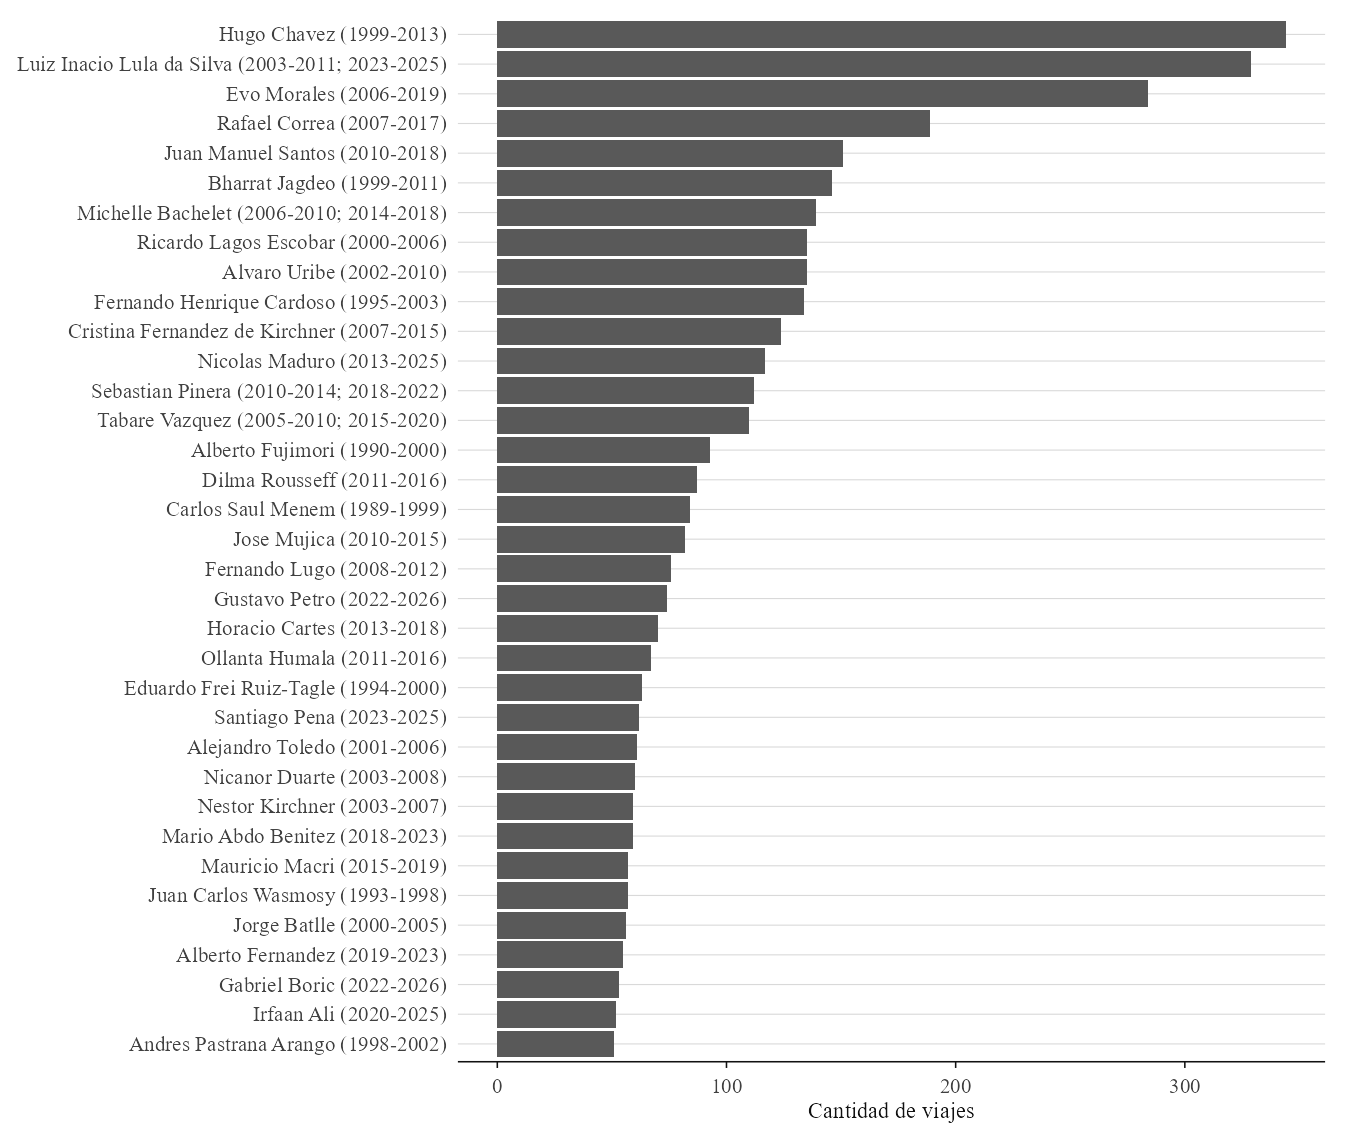
\includegraphics[width=0.9\textwidth]{../08_ANALISIS_R/outputs/00c_viajes_totales_por_mandatario.png}
  \caption{Total de viajes registrados por mandatario, 1994-2025, limitado a mandatarios con m\'as de 50 viajes (la tabla completa, sin ese recorte, est\'a en \texttt{00c\_viajes\_totales\_por\_mandatario.csv}). Entre par\'entesis, el per\'iodo de mandato (dos rangos separados por punto y coma para mandatarios con mandatos no consecutivos). Solo se cuentan viajes realizados durante el mandato (ver Datos y metodolog\'ia).}
  \label{fig:totales-mandatario}
\end{figure}

% latex table generated in R 4.5.1 by xtable 1.8-8 package
% Fri Sep 11 10:51:23 2026
\begin{table}[ht]
\centering
\caption{Estad\'isticos descriptivos (media, desv\'io, m\'inimo, m\'aximo) de viajes por Mandatario-A\~no (total, bilaterales y multilaterales) y de la duraci\'on de los viajes.} 
\label{tab:resumen-estadisticos}
\begingroup\footnotesize
\begin{tabular}{lrrrrrl}
  \hline
variable & media & de & minimo & maximo & n\_obs & Unidad\_n\_obs \\ 
  \hline
Viajes por Mandatario-Anio & 11.80 & 7.90 &   1 &  40 & 425 & Combinaciones mandatario-anio \\ 
  Duracion del viaje (dias) & 2.50 & 2.00 &   1 &  71 & 5000 & Viajes individuales \\ 
  Viajes Bilaterales por Mandatario-Anio & 5.40 & 4.60 &   1 &  27 & 360 & Combinaciones mandatario-anio \\ 
  Viajes Multilaterales por Mandatario-Anio & 5.40 & 3.20 &   1 &  18 & 402 & Combinaciones mandatario-anio \\ 
   \hline
\end{tabular}
\endgroup
\end{table}
% Nota: la base solo incluye viajes realizados DURANTE el mandato (tanto el
% inicio como el fin del viaje deben caer dentro del periodo presidencial;
% ver 08_ANALISIS_R/graficos_exploratorios.R, seccion 1.2c). Por esta regla
% se excluyo el viaje de Jair Bolsonaro a Estados Unidos (30-dic-2022 a
% 30-mar-2023): arranco 2 dias antes de terminar su mandato pero se extendio
% casi 3 meses despues de dejar el cargo. El maximo actual de "Duracion del
% viaje" (71 dias) corresponde a Hugo Chavez, Venezuela a Cuba (10-dic-2012
% a 18-feb-2013) por tratamiento medico -siguio siendo presidente en
% ejercicio durante todo ese periodo, por eso el viaje si queda incluido.
% Nota (correccion pedida por el usuario): las filas de "viajes" del Cuadro
% de arriba agrupan por MANDATARIO-anio (no por pais-anio como en una
% version anterior), separadas en total/bilaterales/multilaterales; la fila
% de duracion no cambio.

\begin{figure}[H]
  \centering
  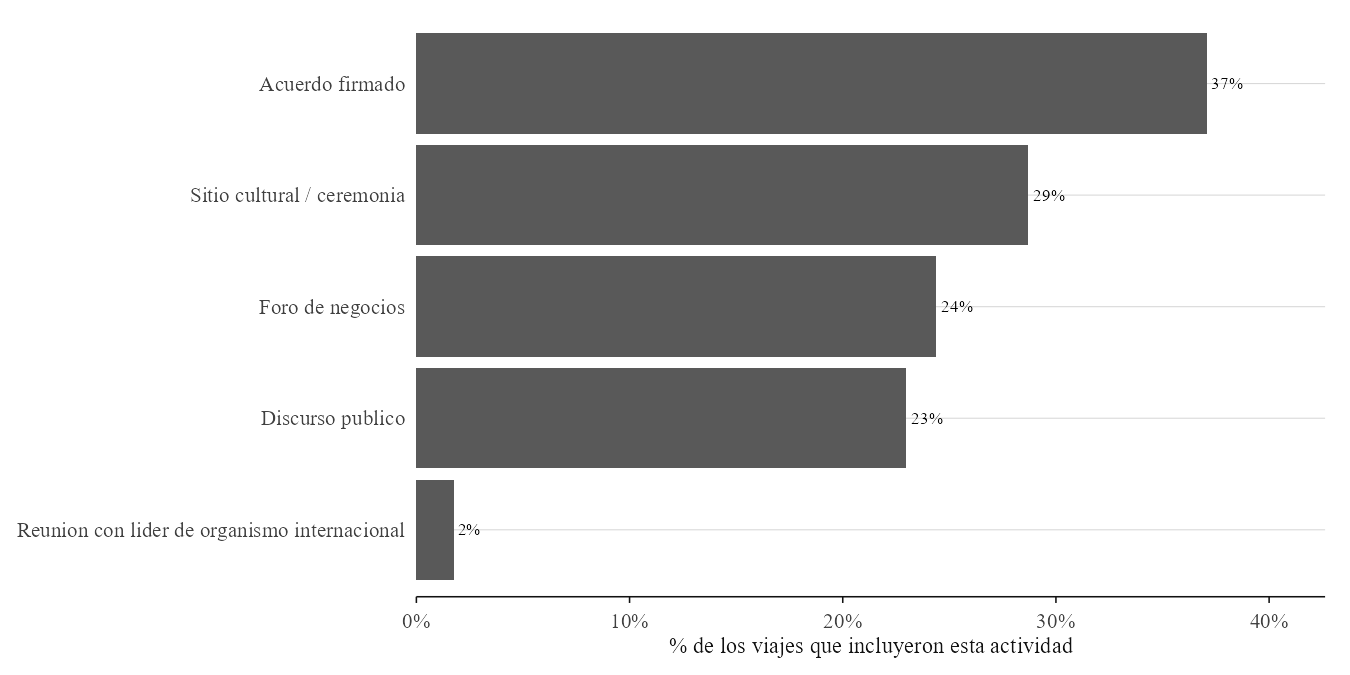
\includegraphics[width=0.75\textwidth]{../08_ANALISIS_R/outputs/12a_tipo_actividad_bilateral.png}
  \caption{Tipo de actividad incluida en los viajes BILATERALES (categor\'ias no excluyentes; cf. \citep{charnockPresidentialTravelEisenhower2009} sobre viajes presidenciales de EE.\,UU.).}
  \label{fig:tipo-actividad-bilateral}
\end{figure}

\begin{figure}[H]
  \centering
  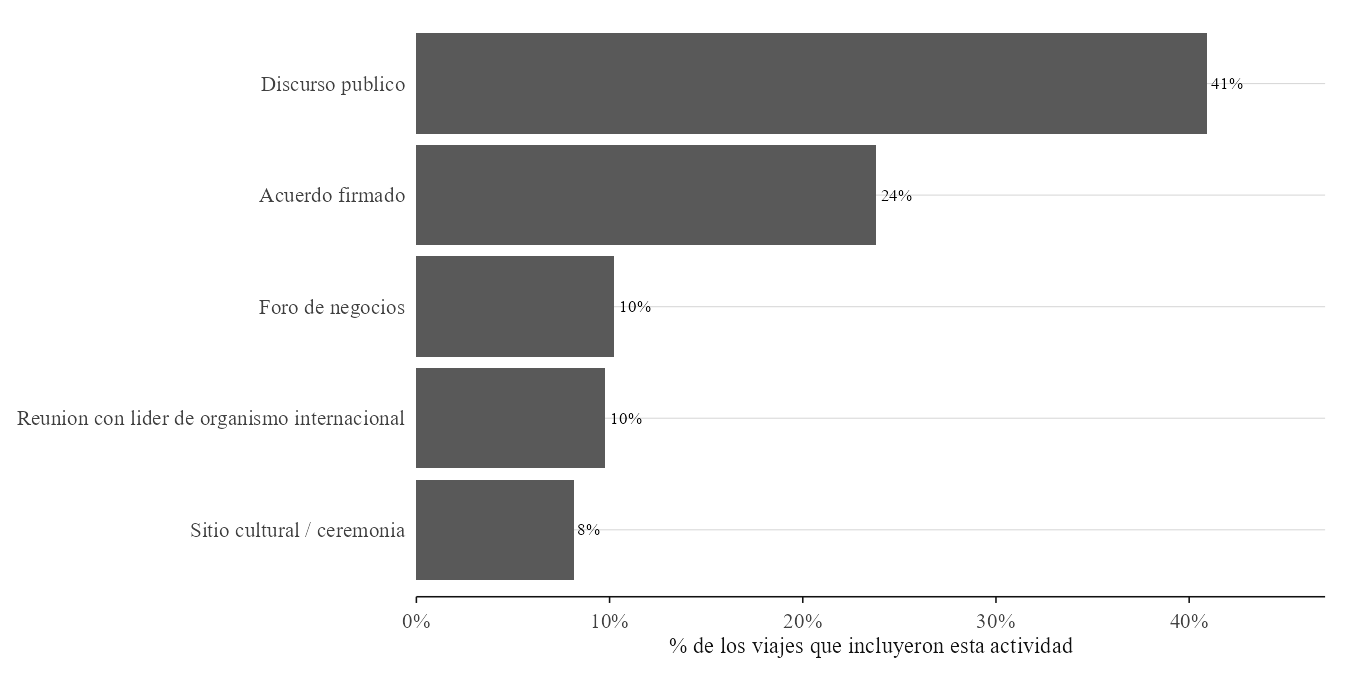
\includegraphics[width=0.75\textwidth]{../08_ANALISIS_R/outputs/12b_tipo_actividad_multilateral.png}
  \caption{Tipo de actividad incluida en los viajes MULTILATERALES (categor\'ias no excluyentes).}
  \label{fig:tipo-actividad-multilateral}
\end{figure}

\begin{figure}[H]
  \centering
  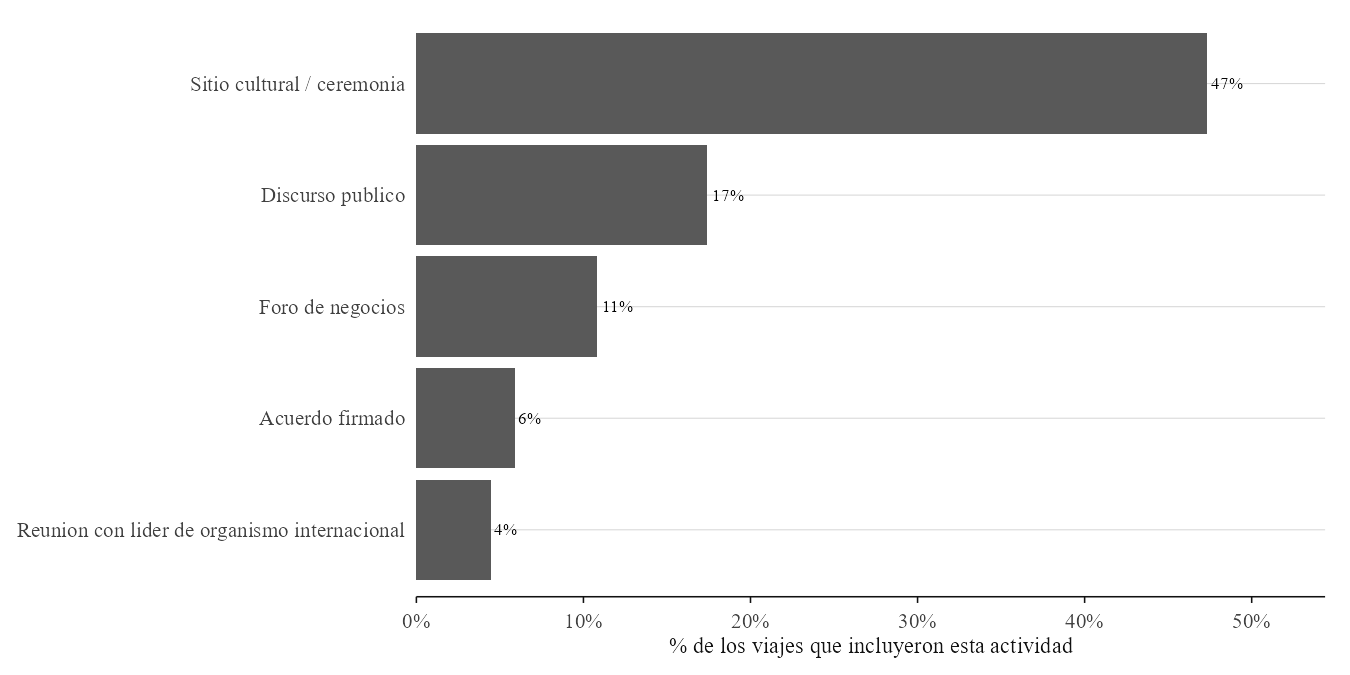
\includegraphics[width=0.75\textwidth]{../08_ANALISIS_R/outputs/12c_tipo_actividad_otro.png}
  \caption{Tipo de actividad incluida en los viajes de categor\'ia ``Otro'' (categor\'ias no excluyentes). Separar por categor\'ia de visita (Bilateral/Multilateral/Otro; a diferencia de una versi\'on anterior de esta figura, que mezclaba las tres) permite ver que actividades predominan seg\'un el motivo del viaje.}
  \label{fig:tipo-actividad-otro}
\end{figure}

\subsubsection{Evoluci\'on temporal}

\begin{figure}[H]
  \centering
  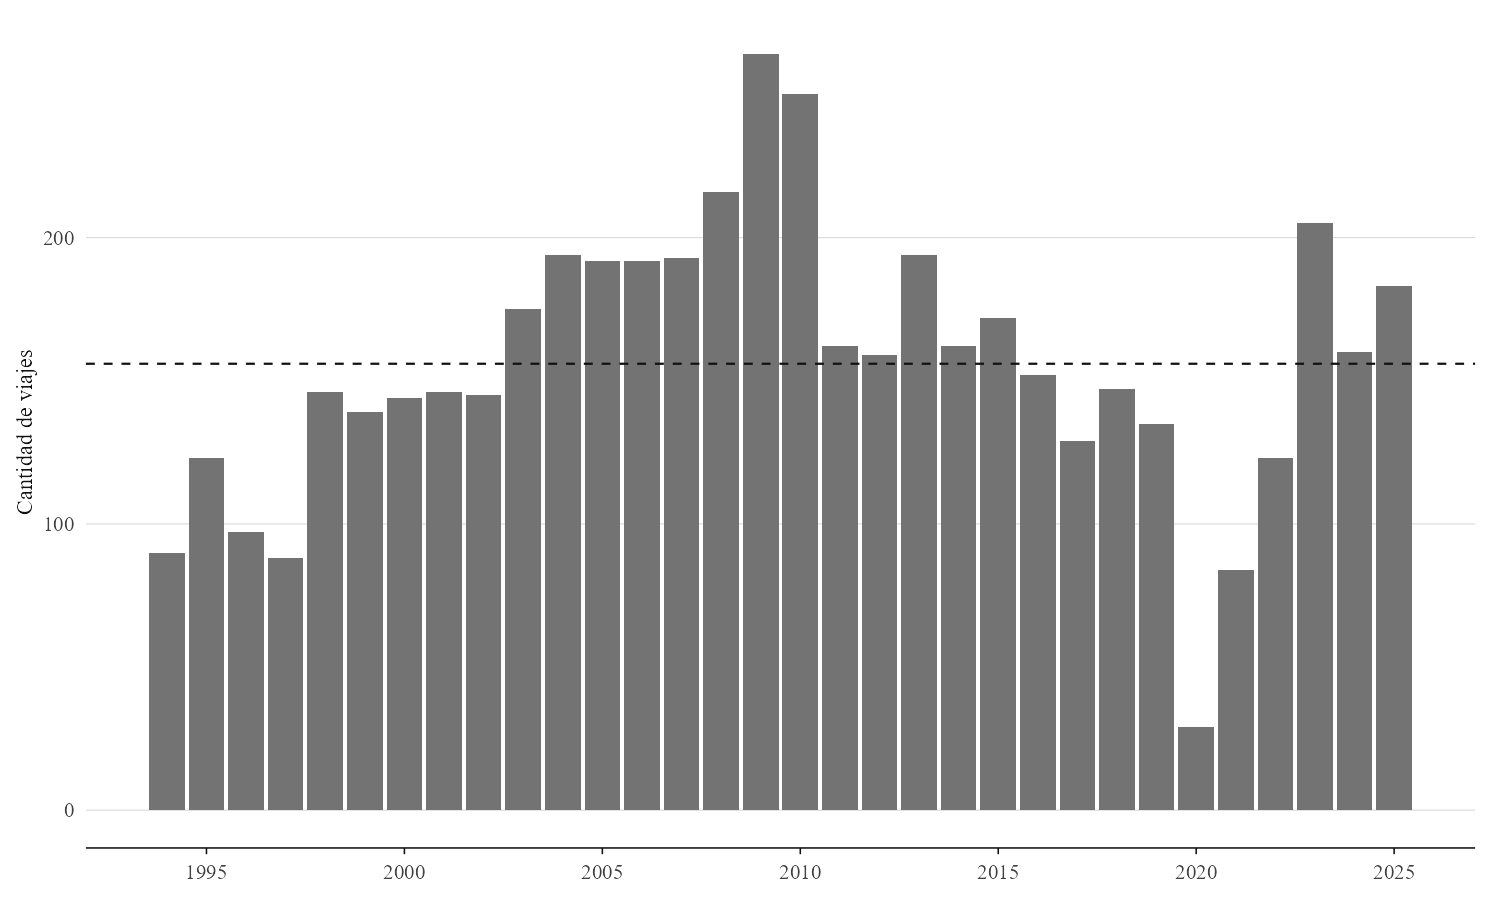
\includegraphics[width=0.85\textwidth]{../08_ANALISIS_R/outputs/01_viajes_por_anio.png}
  \caption{Cantidad de viajes presidenciales por a\~no, Sudam\'erica 1994-2025. La l\'inea punteada marca el promedio anual de todo el per\'iodo.}
  \label{fig:viajes-por-anio}
\end{figure}

\begin{figure}[H]
  \centering
  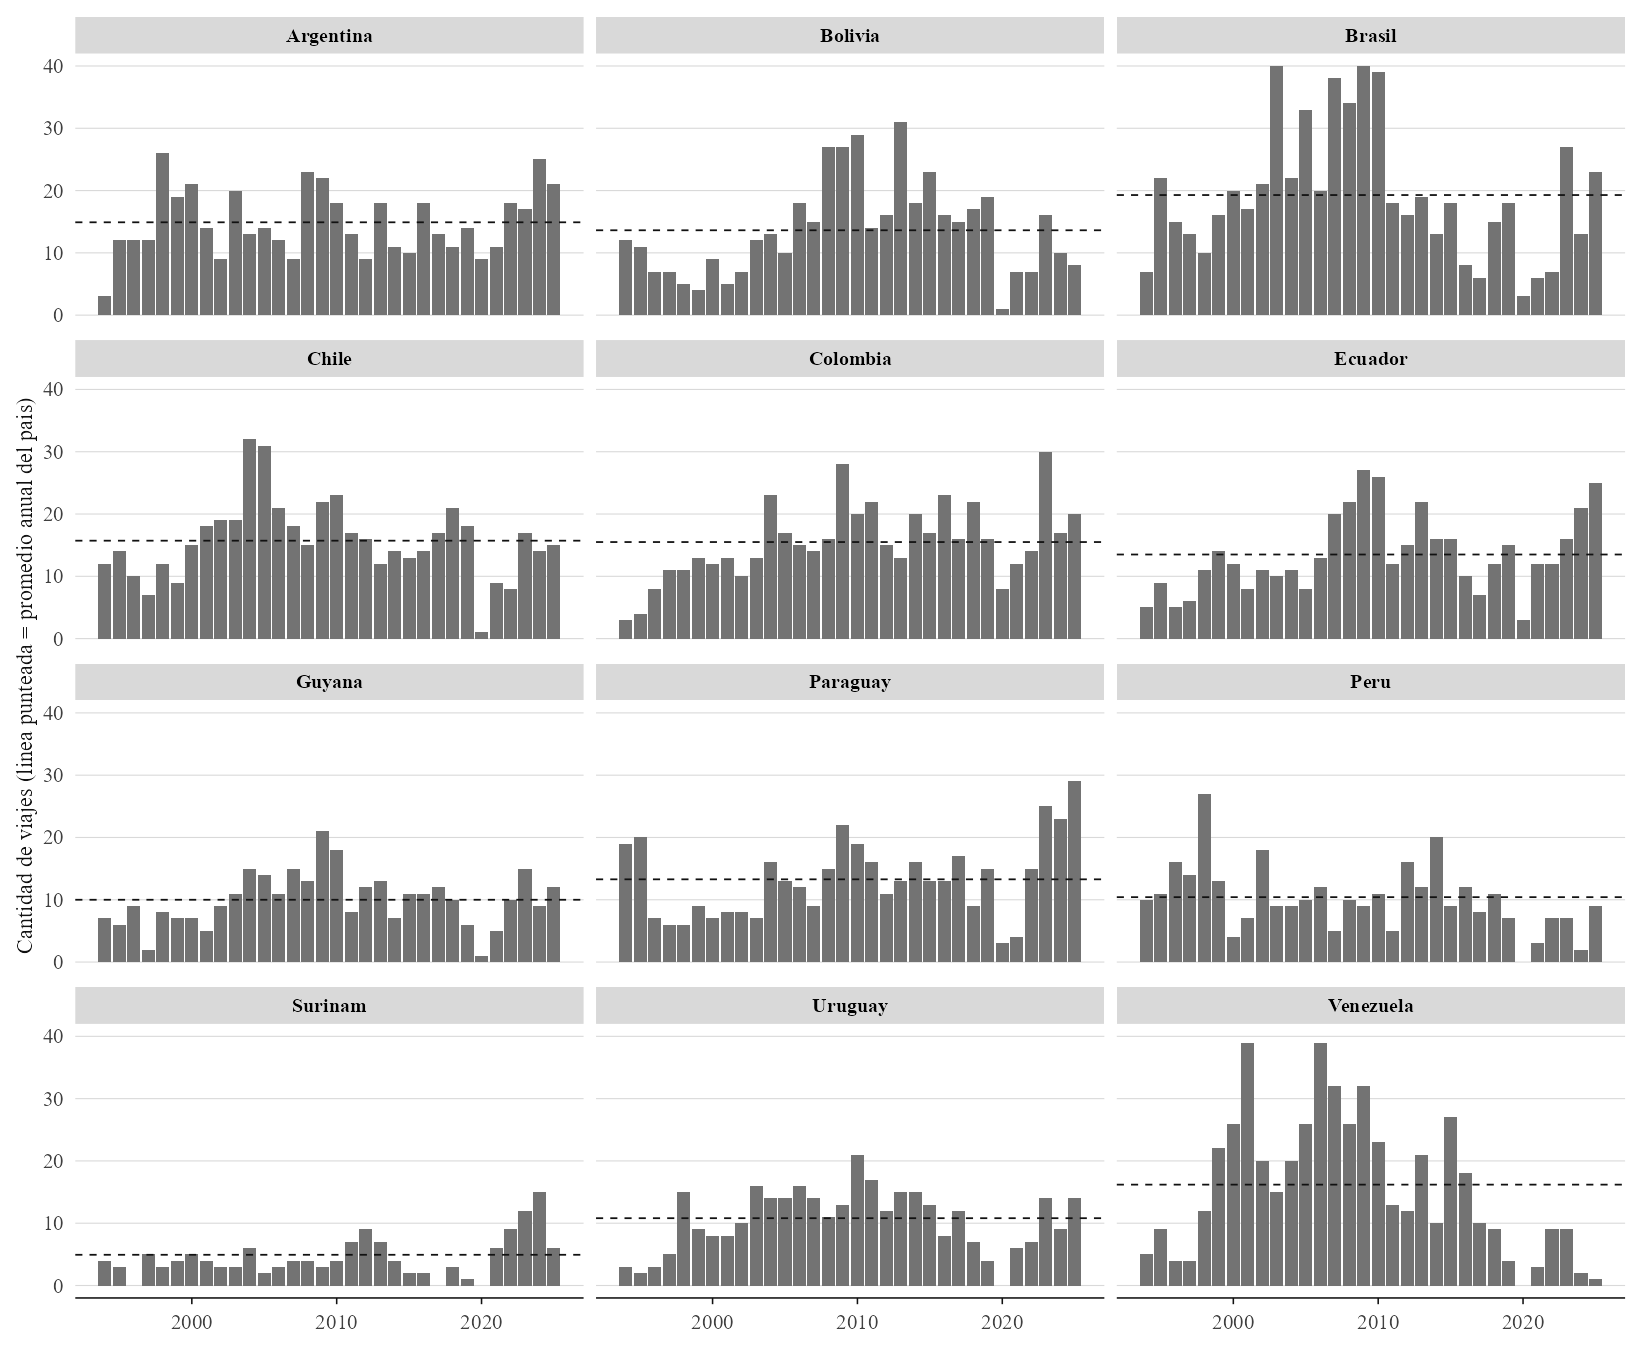
\includegraphics[width=\textwidth]{../08_ANALISIS_R/outputs/01b_viajes_por_anio_por_pais.png}
  \caption{Cantidad de viajes por a\~no, desagregado por pa\'is. La l\'inea punteada marca el promedio anual de cada pa\'is.}
  \label{fig:viajes-por-anio-pais}
\end{figure}

% Figura 7 anterior (11_viajes_por_anio_de_mandato.png, promedio de viajes
% por anio de mandato) ELIMINADA del paper a pedido del usuario (2026-09-06).
% El PNG y el codigo que lo genera se mantienen en graficos_exploratorios.R
% por si se quiere reincorporar mas adelante.

\begin{figure}[H]
  \centering
  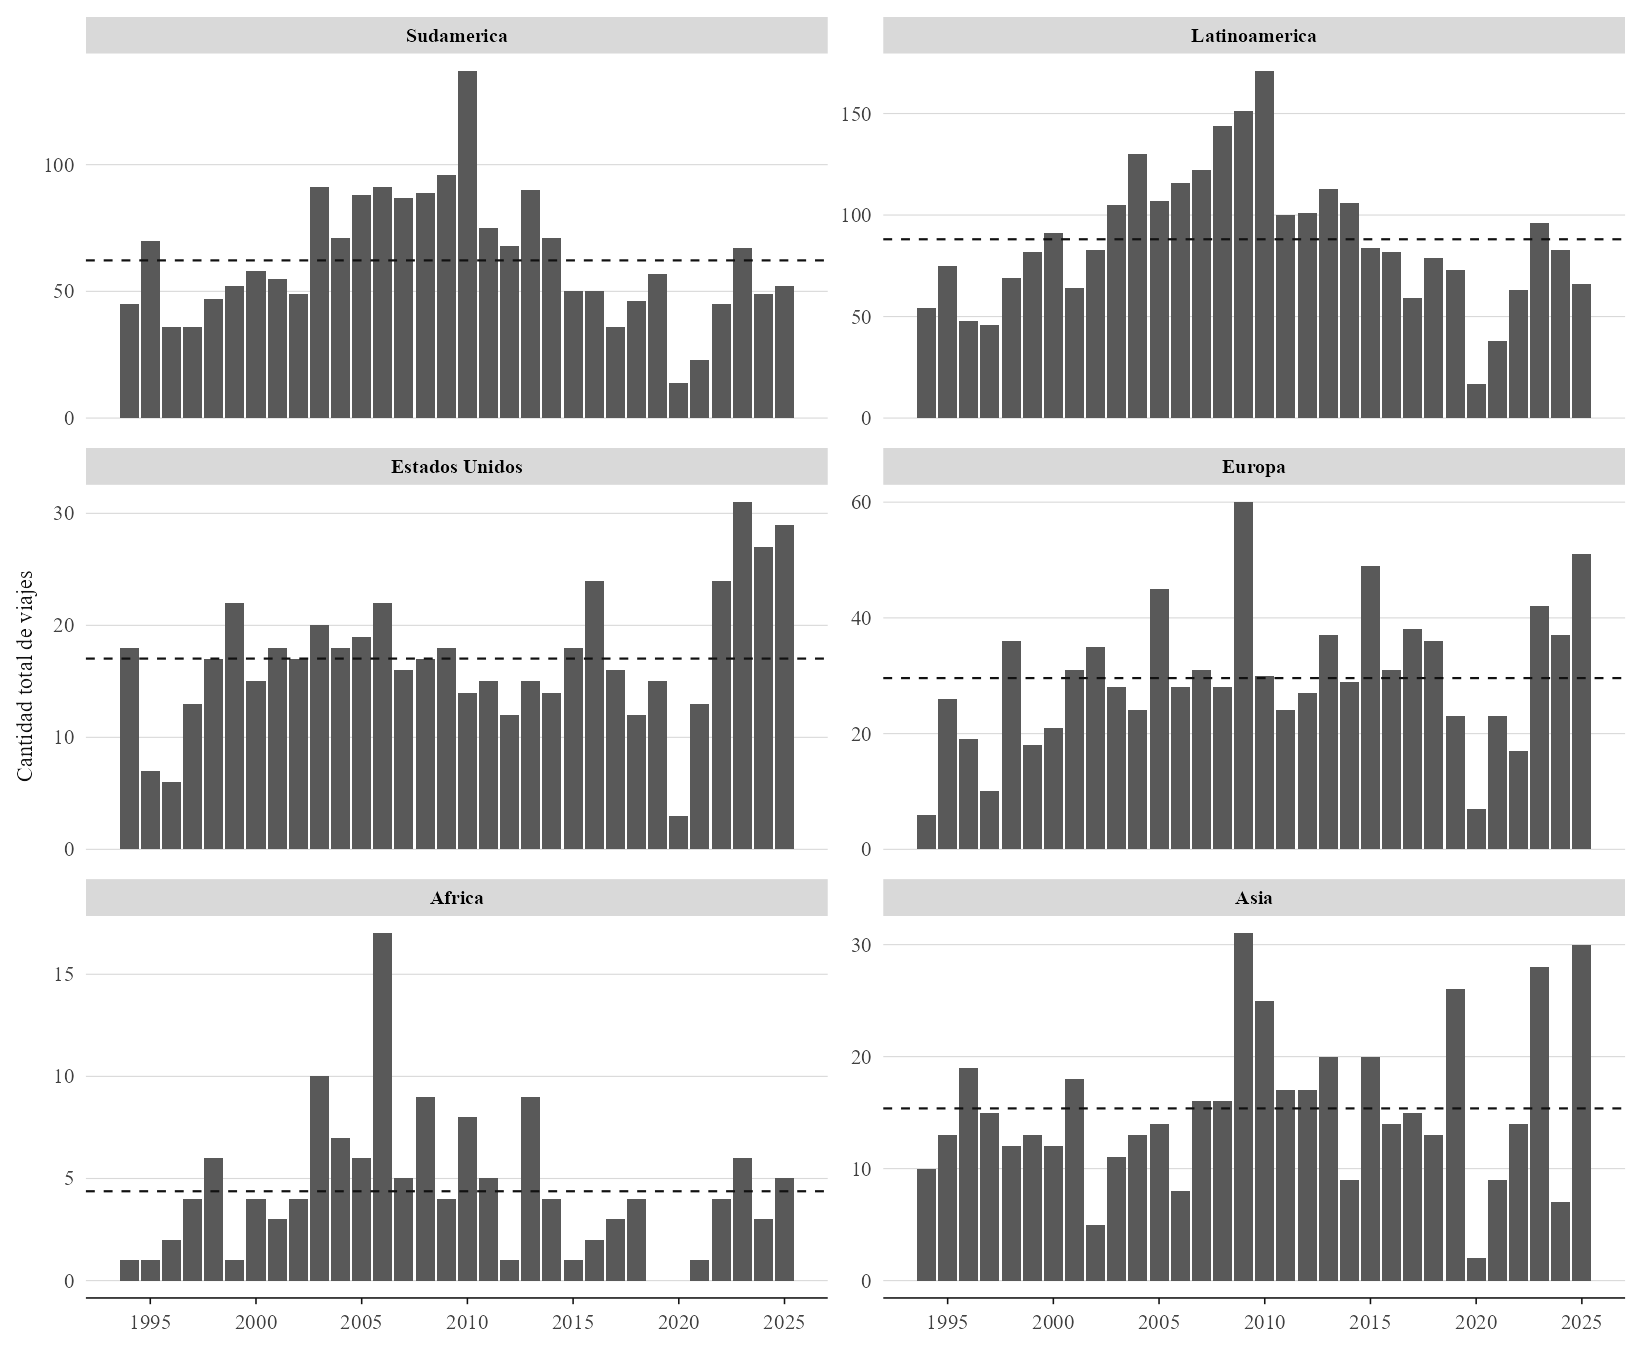
\includegraphics[width=\textwidth]{../08_ANALISIS_R/outputs/15_evolucion_por_bloque_destino.png}
  \caption{Cantidad total de viajes por a\~no a cada bloque de destino: Sudam\'erica, Latinoam\'erica y el Caribe (incluye a Sudam\'erica), Estados Unidos, Europa, \'Africa y Asia. Sudam\'erica y Latinoam\'erica se superponen a prop\'osito -la segunda incluye a la primera-, para comparar el volumen dentro de la vecindad m\'as cercana contra el de la regi\'on en un sentido amplio. La l\'inea punteada marca el promedio anual de cada bloque (1994-2025).}
  \label{fig:evolucion-por-bloque-destino}
\end{figure}

% NOTA (2026-09-06): estilo editorial que rompia a proposito la estetica Q1
% (titulo/subtitulo/fuente adentro de la imagen, replicando un grafico de
% referencia de Diplometrics COLT) DESCARTADO a pedido del usuario. Esta
% figura ahora usa el mismo grafico base que el resto del paper
% (17_integracion_regional_en_retirada.png regenerado en graficos_exploratorios.R
% con el tema Q1 estandar) y la etiqueta de Minimo ya no queda cortada.
\begin{figure}[H]
  \centering
  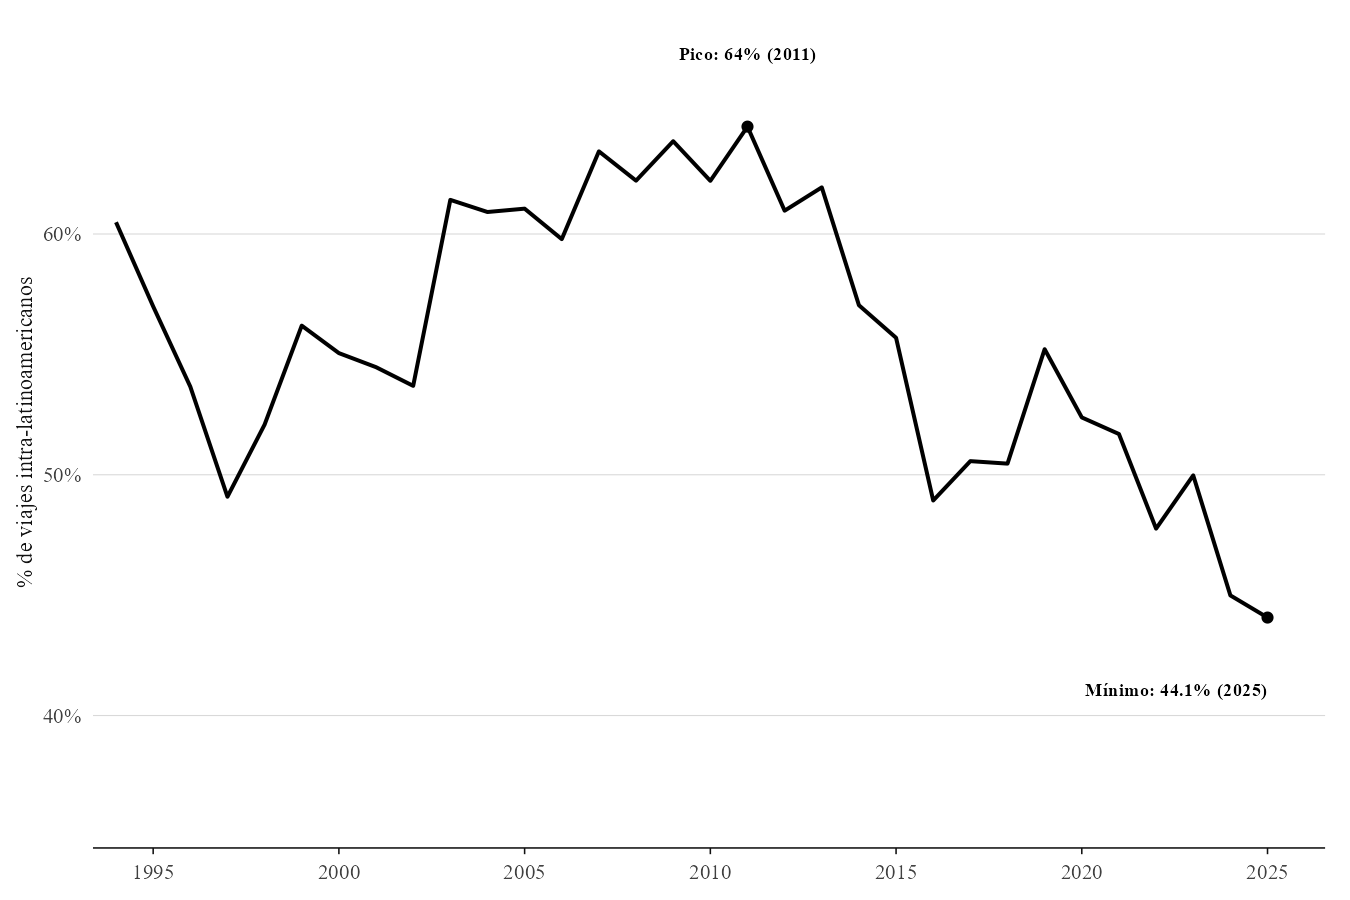
\includegraphics[width=0.8\textwidth]{../08_ANALISIS_R/outputs/17_integracion_regional_en_retirada.png}
  \caption{Participaci\'on de los viajes intra-latinoamericanos sobre el total de viajes presidenciales sudamericanos, promedio m\'ovil de 3 a\~nos, 1994-2025. Recreaci\'on propia -con nuestra base cruzada y verificada- de un gr\'afico de referencia de Diplometrics COLT (que usa datos crudos 1990-2025); no extendemos a 1990-1993 porque la cobertura verificada de varios pa\'ises de nuestra base no llega de forma confiable a esos a\~nos. El patr\'on se sostiene: pico y m\'inimo caen en los mismos a\~nos que en la fuente de referencia (2011 y 2025).}
  \label{fig:integracion-regional-en-retirada}
\end{figure}

% Mismo estilo que la Figura~\ref{fig:evolucion-por-bloque-destino} (facet_wrap
% con promedio por panel), pero mirando quien RECIBE los viajes en vez de a
% donde viajan los presidentes. Solo viajes Bilaterales (visita puntual
% dirigida a ese pais, no cumbres multilaterales alojadas ahi).
\begin{figure}[H]
  \centering
  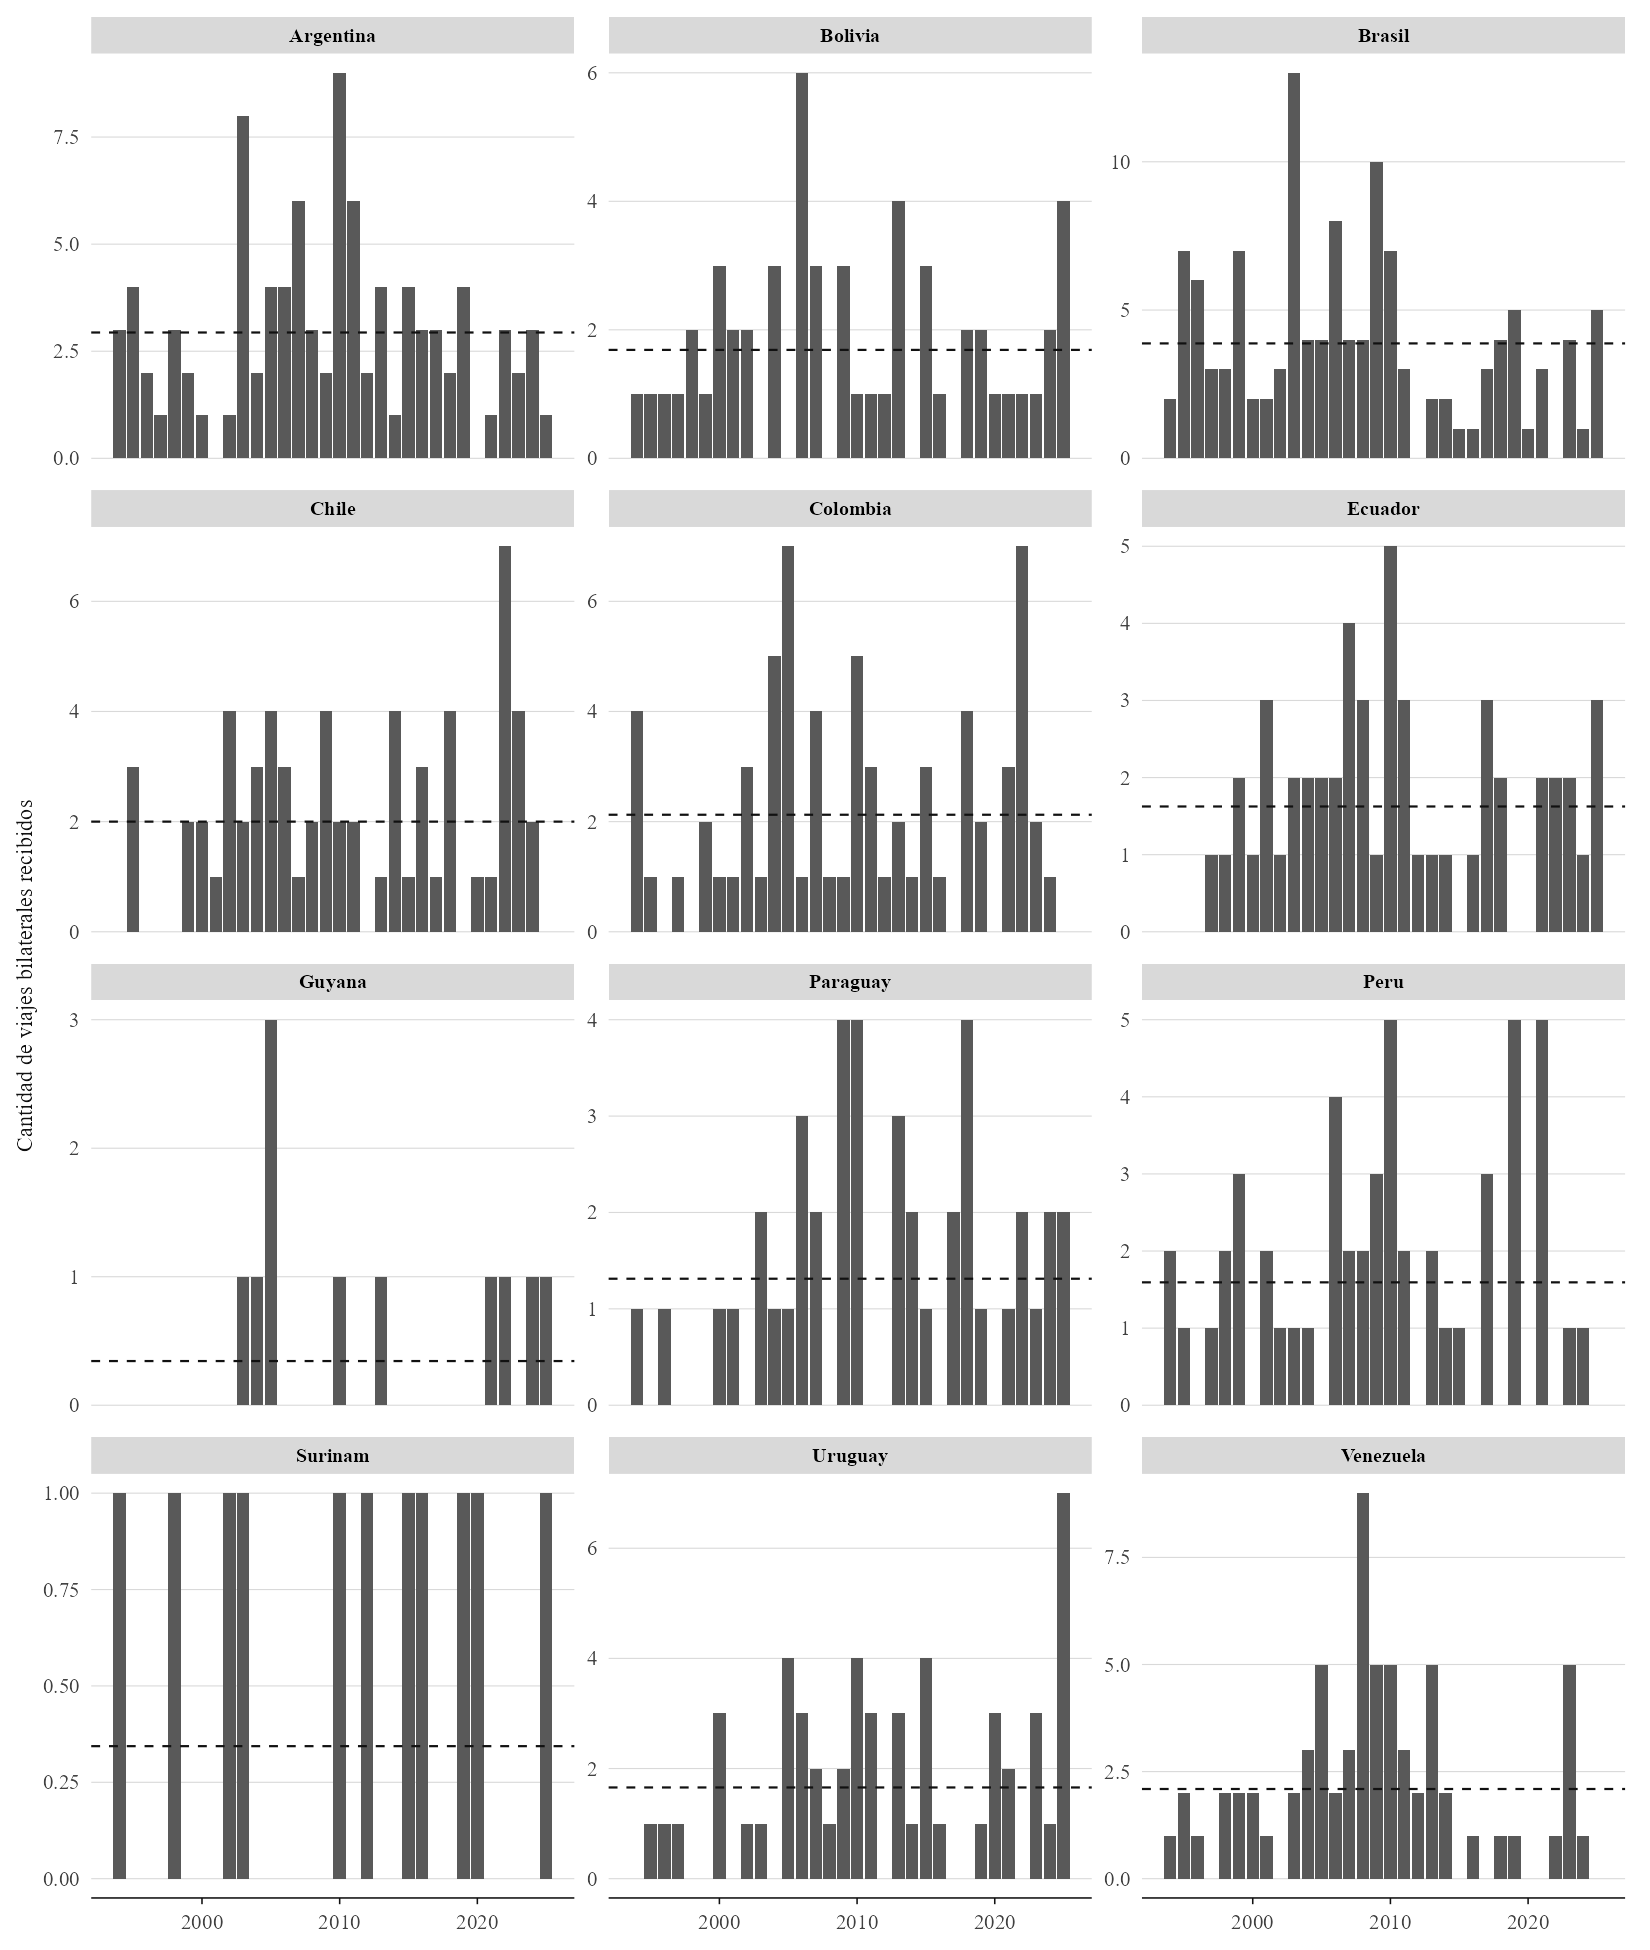
\includegraphics[width=\textwidth]{../08_ANALISIS_R/outputs/17b_viajes_recibidos_intra_sudamerica.png}
  \caption{Cantidad de viajes BILATERALES recibidos por a\~no por cada pa\'is sudamericano, de mandatarios de otros pa\'ises sudamericanos (1994-2025). Cada panel es un pa\'is de destino, todos con la MISMA escala en el eje Y (a diferencia de la Figura~\ref{fig:evolucion-por-bloque-destino}, que usa escala libre por panel) para poder comparar directamente cu\'anto recibe cada pa\'is frente a los dem\'as; la l\'inea punteada marca el promedio anual propio de cada pa\'is. Permite ver qu\'e pa\'ises ganan o pierden peso como destino de la diplomacia bilateral de sus vecinos a lo largo del tiempo.}
  \label{fig:viajes-recibidos-intra-sudamerica}
\end{figure}

\begin{figure}[H]
  \centering
  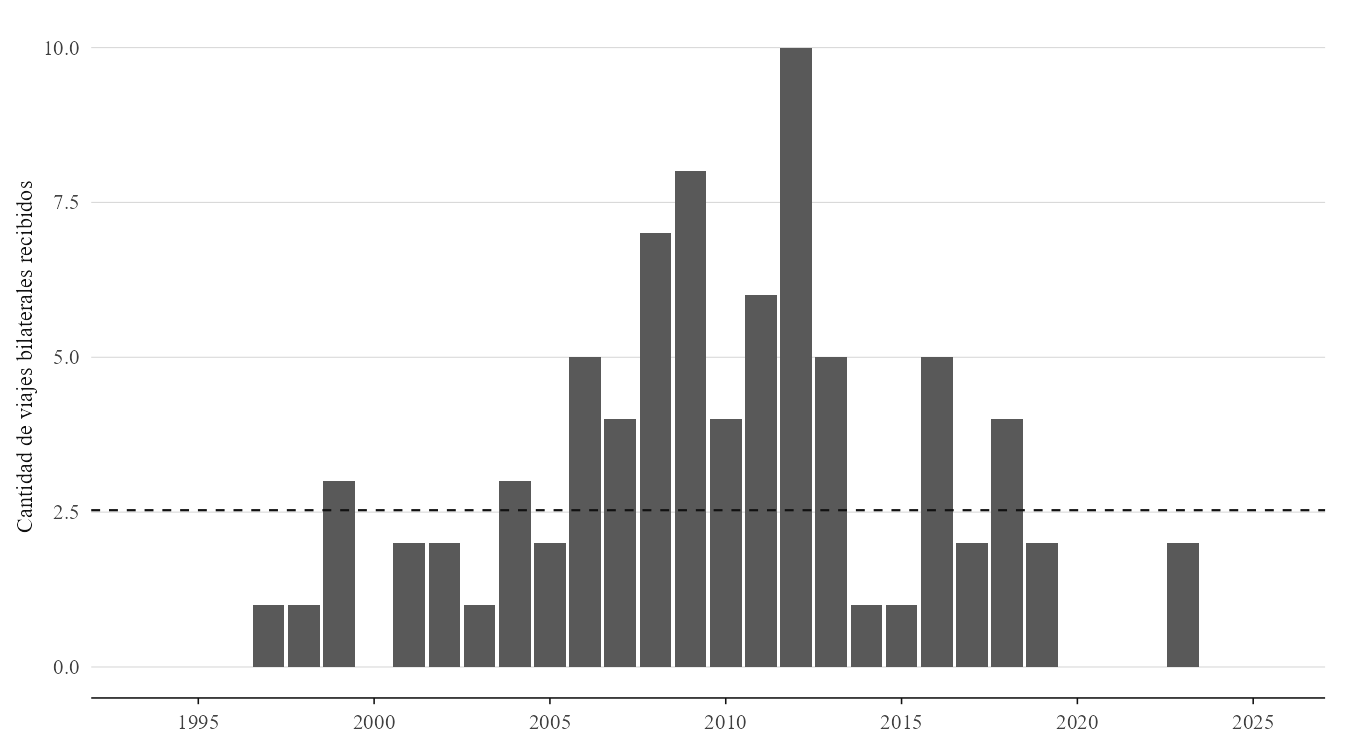
\includegraphics[width=0.75\textwidth]{../08_ANALISIS_R/outputs/17c_viajes_recibidos_cuba.png}
  \caption{Cantidad de viajes BILATERALES recibidos por Cuba de mandatarios sudamericanos, por a\~no (1994-2025). Cuba no es un pa\'is sudamericano -por eso queda fuera de la grilla de la Figura~\ref{fig:viajes-recibidos-intra-sudamerica}- pero se incluye aparte por su peso simb\'olico/hist\'orico como destino de la diplomacia sudamericana. La l\'inea punteada marca el promedio anual del per\'iodo.}
  \label{fig:viajes-recibidos-cuba}
\end{figure}

\begin{figure}[H]
  \centering
  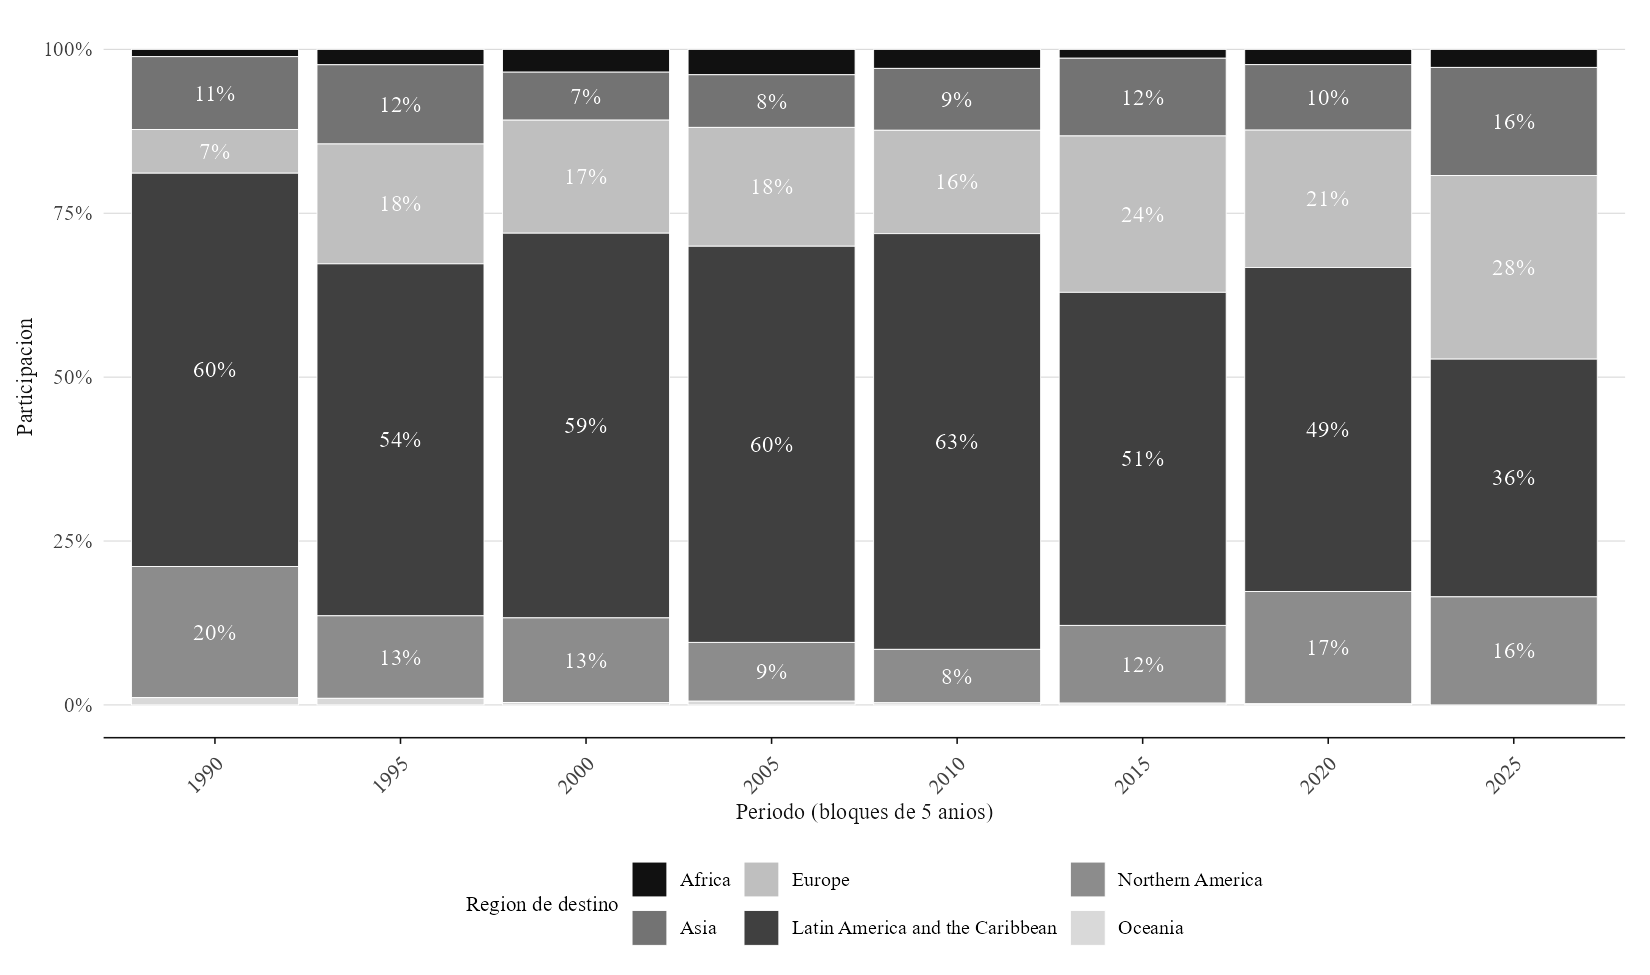
\includegraphics[width=0.9\textwidth]{../08_ANALISIS_R/outputs/02_regiones_por_periodo.png}
  \caption{Prioridad regional de los viajes presidenciales, por per\'iodo (bloques de 5 a\~nos). Etiquetas de dato para Am\'erica Latina y el Caribe, Europa y Norteam\'erica.}
  \label{fig:regiones-periodo}
\end{figure}

% Figuras "regiones por anio" (area apilada) y "duracion por anio" ELIMINADAS
% (pedido del usuario): la primera duplicaba la Figura~\ref{fig:regiones-periodo}
% a nivel anual sin agregar informacion nueva; la segunda queda cubierta por
% la Figura~\ref{fig:viajes-duracion-combinado} (viajes + duracion en un solo
% grafico).

\begin{figure}[H]
  \centering
  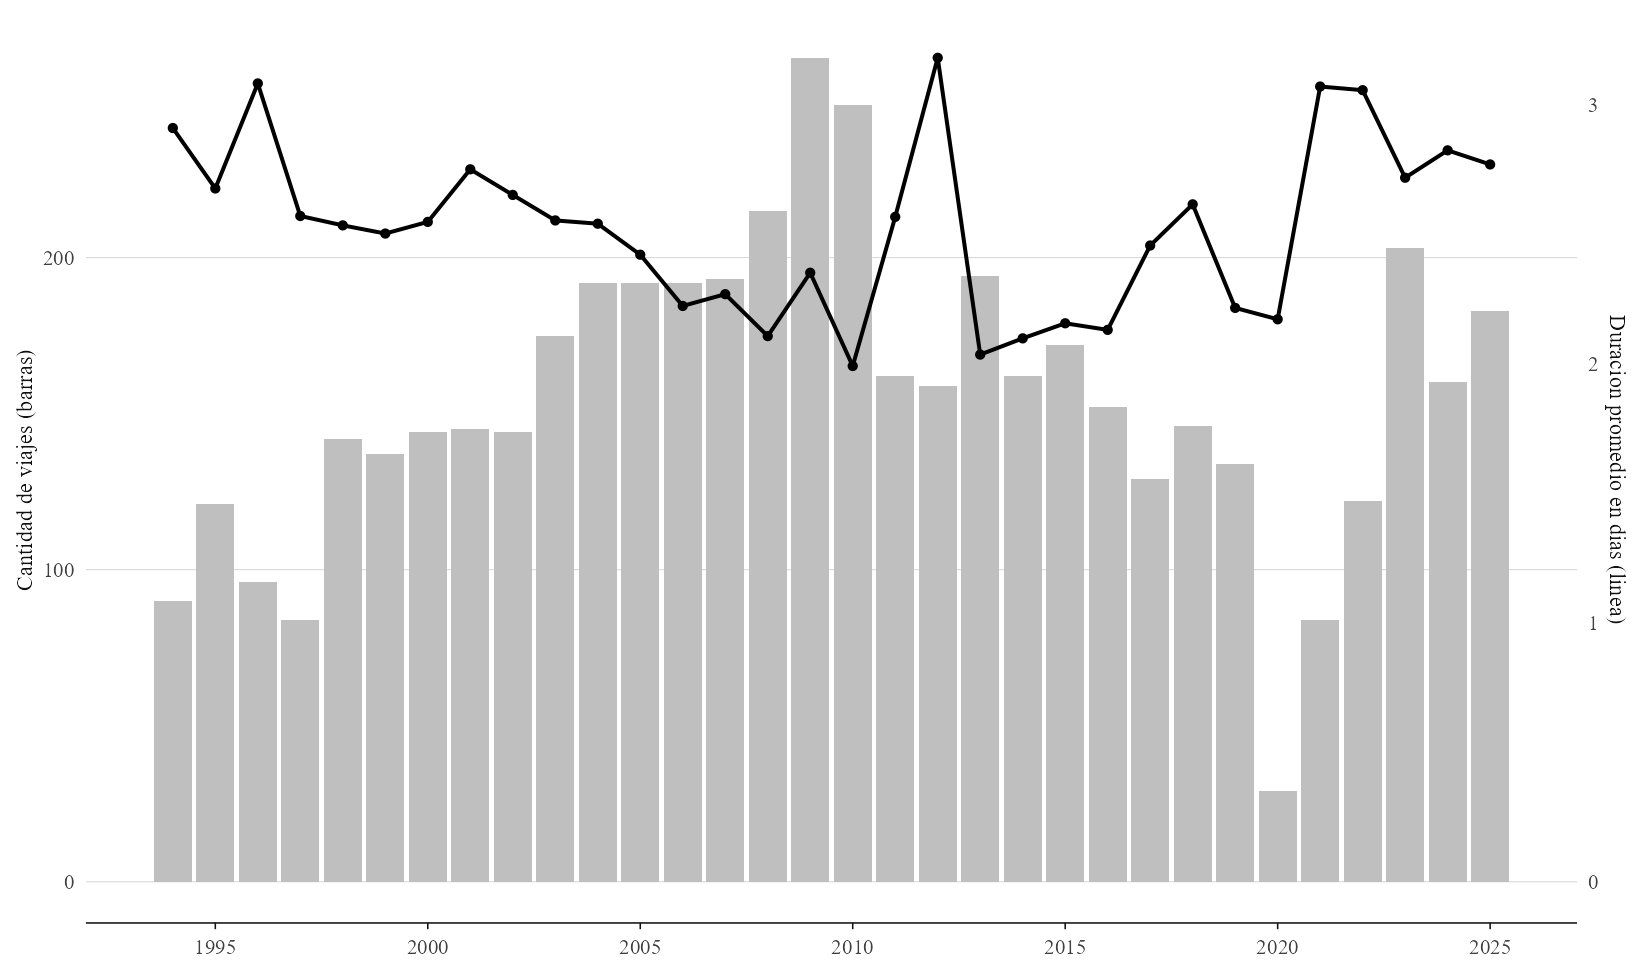
\includegraphics[width=0.9\textwidth]{../08_ANALISIS_R/outputs/03c_viajes_y_duracion_combinado.png}
  % Resaltado amarillo agregado 2026-09-10 (pedido del usuario, item 6):
  % contenido probablemente se saque en una version futura -revisar antes
  % de la version final-. \parbox evita el bug de Overfull hbox que tenia
  % Figura 19/Cuadro 10 con colorbox envolviendo todo el caption sin quiebre
  % de linea.
  \caption{\colorbox{yellow}{\parbox{\dimexpr\textwidth-2\fboxsep\relax}{Cantidad de viajes (barras) y duraci\'on promedio en d\'ias (l\'inea), por a\~no.}}}
  \label{fig:viajes-duracion-combinado}
\end{figure}

\begin{figure}[H]
  \centering
  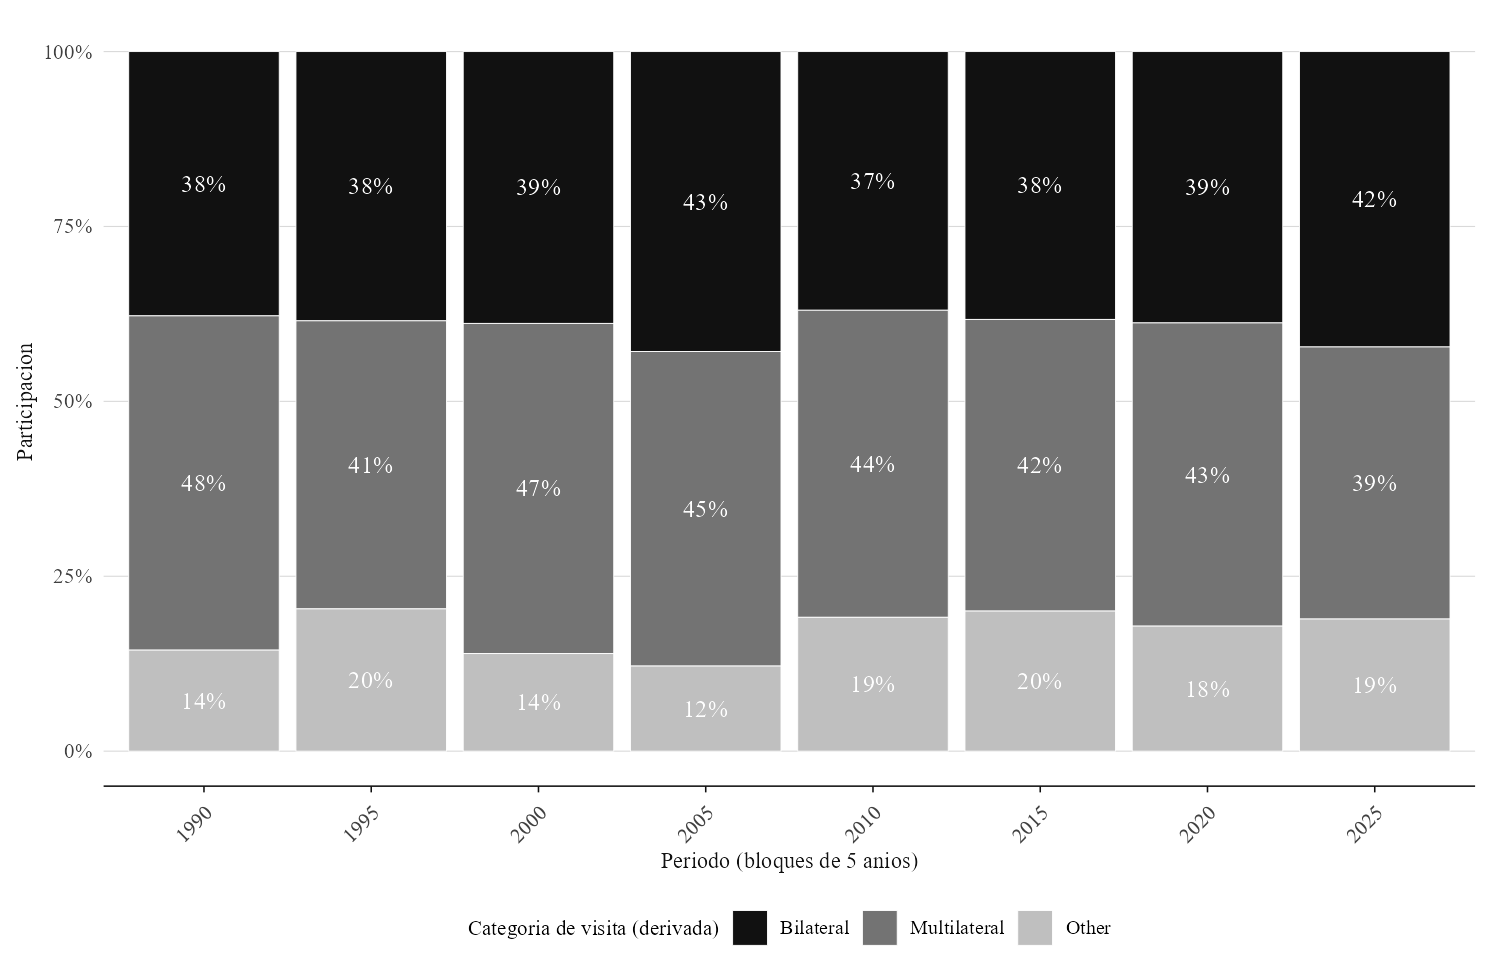
\includegraphics[width=0.85\textwidth]{../08_ANALISIS_R/outputs/04_categoria_visita_por_anio.png}
  \caption{Participaci\'on de Bilateral / Multilateral / Otro, por per\'iodo (bloques de 5 a\~nos; mismo formato que la Figura~\ref{fig:regiones-periodo}). ``Otro'' = sin reuni\'on registrada con el anfitri\'on ni asistencia a un evento multilateral. Se excluyen los viajes sin dato suficiente para clasificar la categor\'ia (``Sin dato'', ver Datos y metodolog\'ia) hasta resolver esa cobertura.}
  \label{fig:categoria-anio}
\end{figure}

\begin{figure}[H]
  \centering
  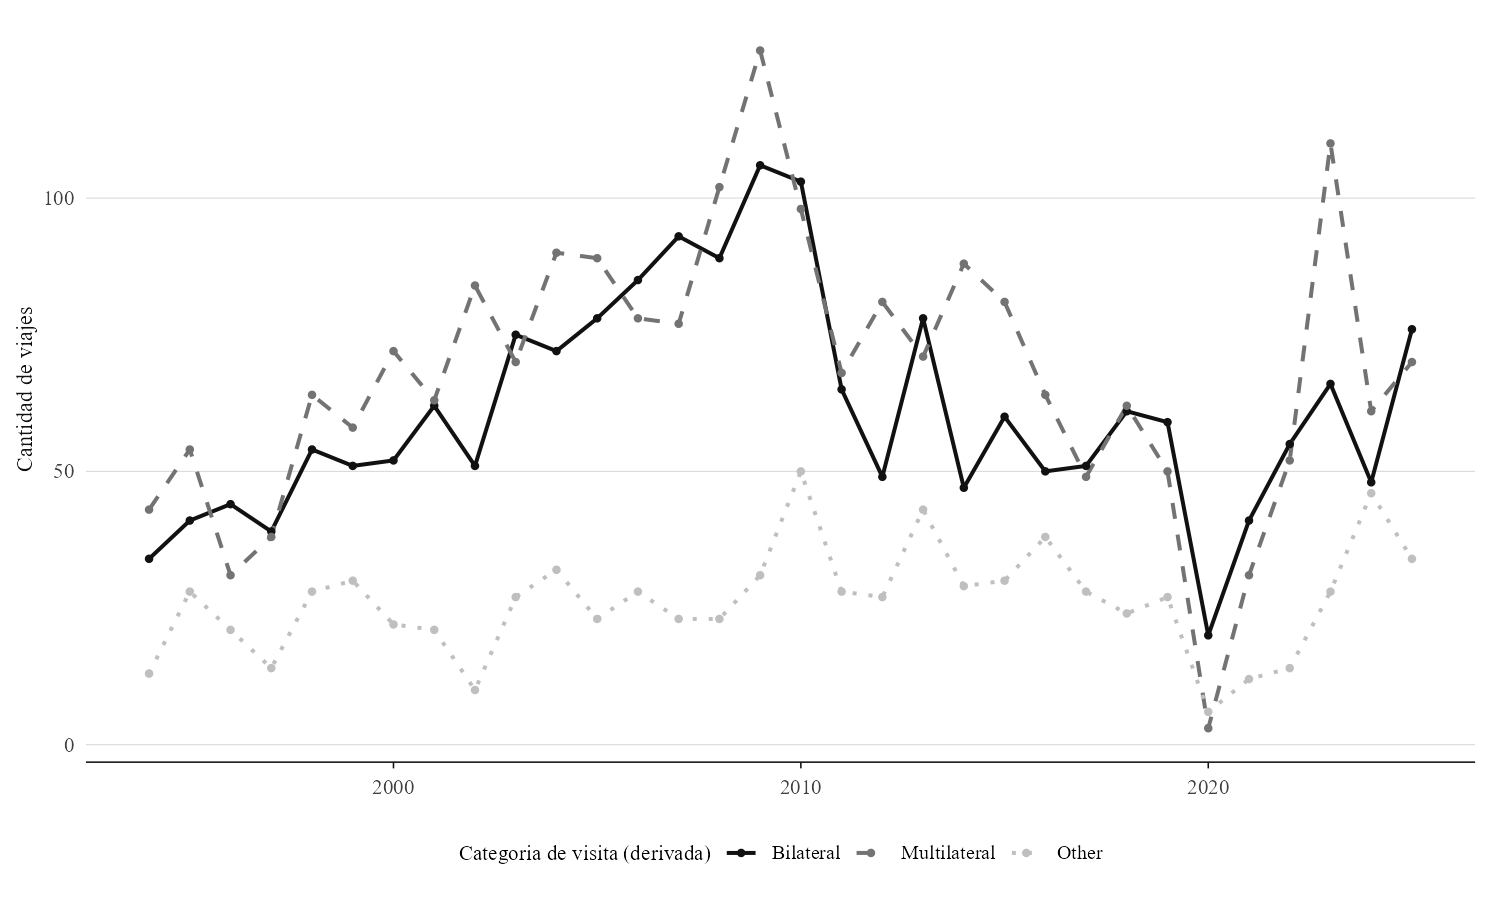
\includegraphics[width=0.85\textwidth]{../08_ANALISIS_R/outputs/04b_categoria_visita_absoluto.png}
  \caption{Cantidad absoluta de viajes por categor\'ia (Bilateral/Multilateral/Otro), por a\~no. Se excluyen los viajes de categor\'ia ``Sin dato'' hasta resolver esa cobertura.}
  \label{fig:categoria-absoluto}
\end{figure}

\begin{figure}[H]
  \centering
  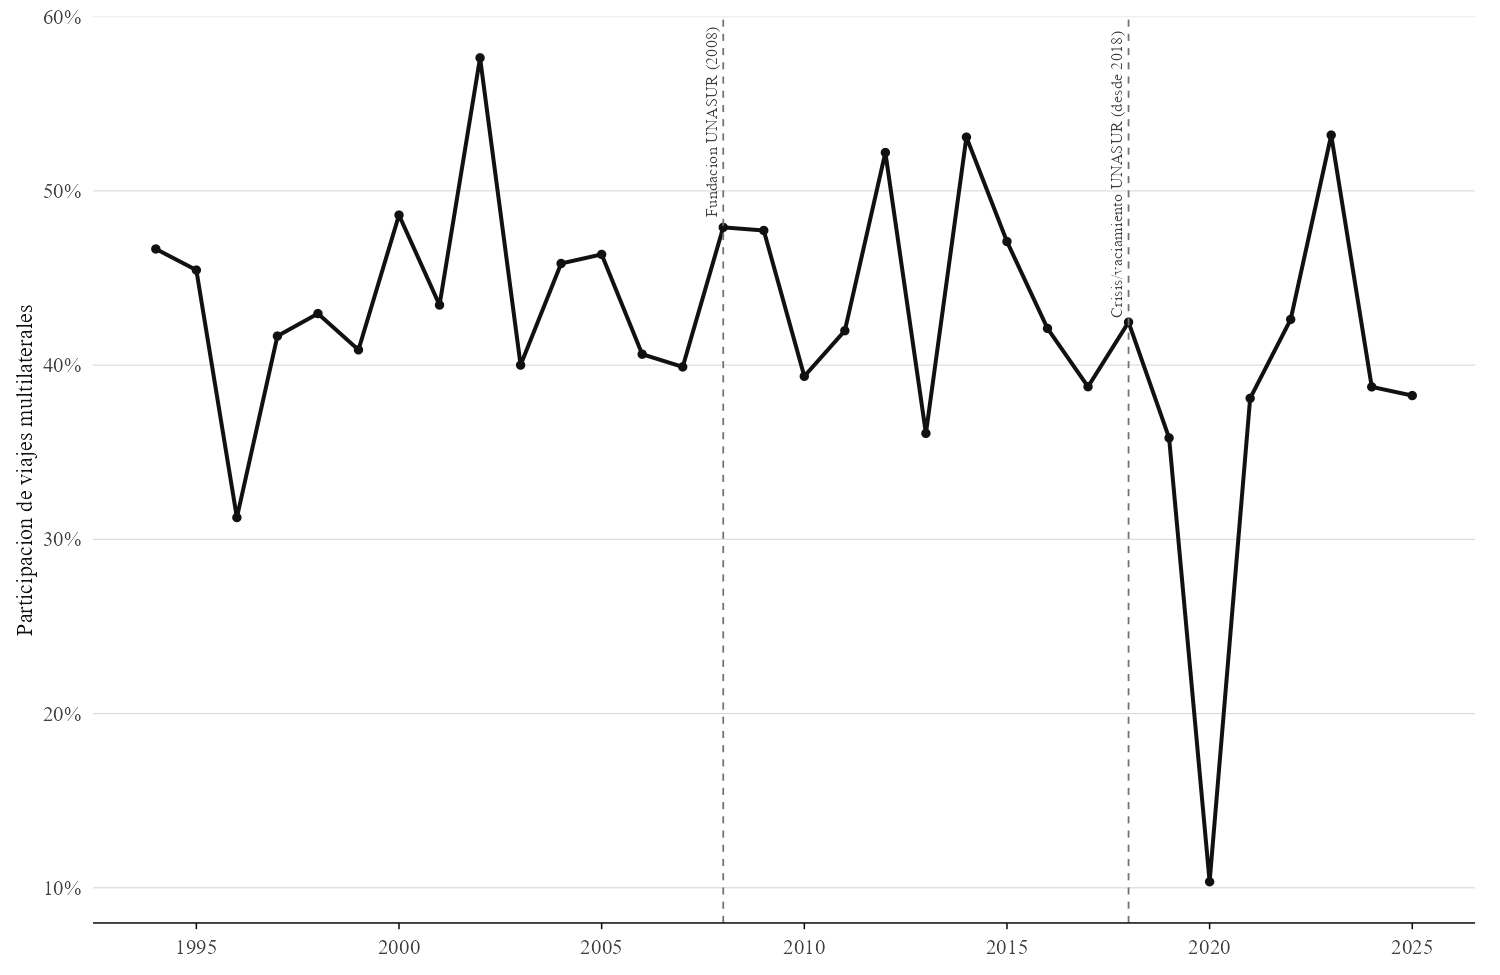
\includegraphics[width=0.85\textwidth]{../08_ANALISIS_R/outputs/13_auge_caida_multilateralismo.png}
  \caption{Participaci\'on de viajes multilaterales por a\~no, con hitos de multilateralismo regional marcados como referencia: la Comunidad Sudamericana de Naciones y la ALBA (2004), la fundaci\'on de UNASUR (2008), la fundaci\'on de la CELAC (2011), la crisis/vaciamiento de UNASUR (desde 2018) y la fundaci\'on de PROSUR (2019) (cf. \citep{nolteSummitsPlainsCrisis2021, barrosCrisisSouthAmerican2021}).}
  \label{fig:auge-caida-multilateralismo}
\end{figure}

\begin{figure}[H]
  \centering
  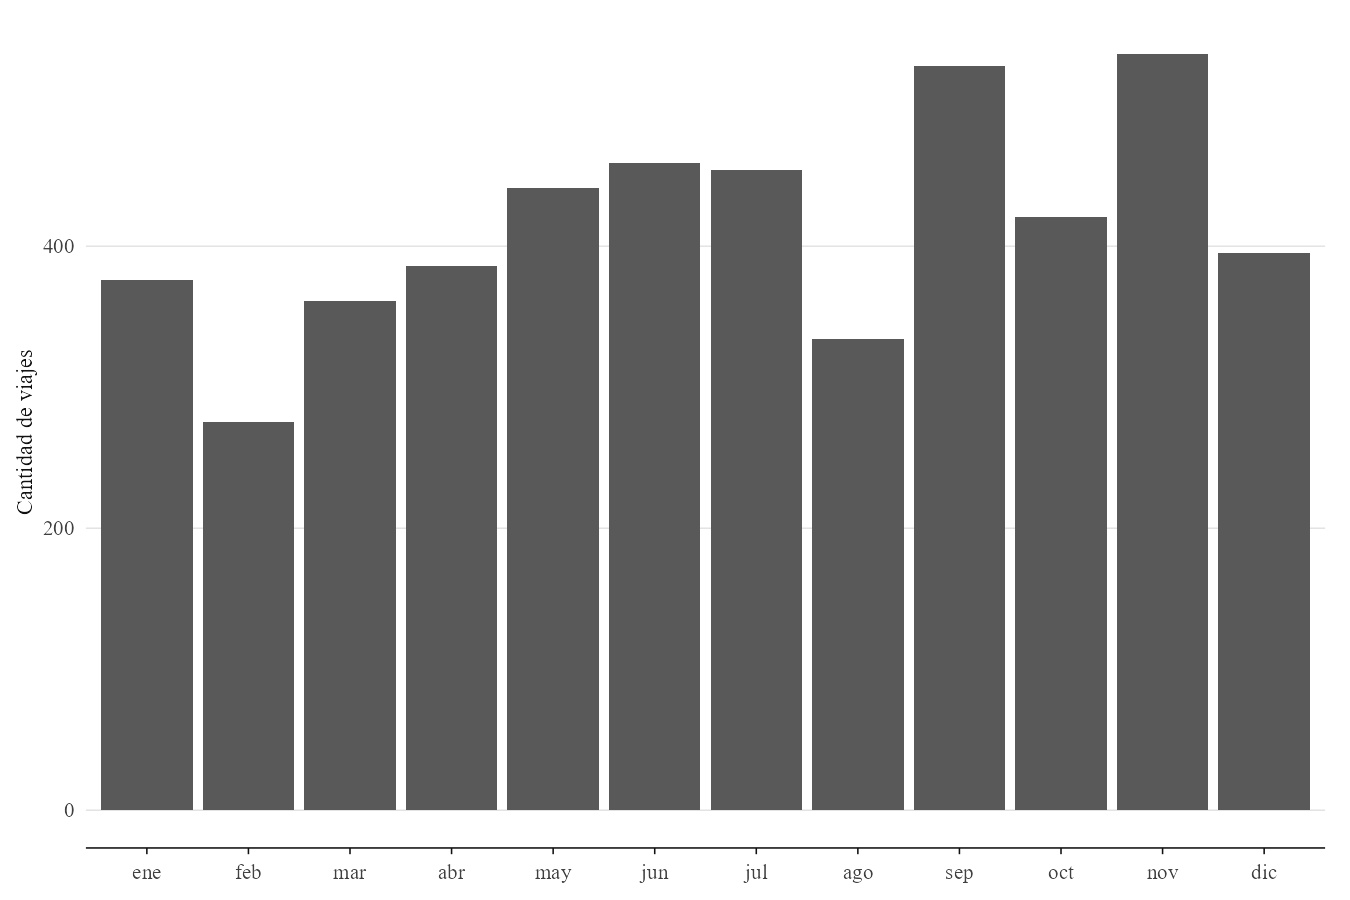
\includegraphics[width=0.85\textwidth]{../08_ANALISIS_R/outputs/08_estacionalidad_mensual.png}
  % Resaltado amarillo agregado 2026-09-10 (pedido del usuario, item 7):
  % mismo criterio y mismo fix de overflow que Figura 12 (ver comentario ahi).
  \caption{\colorbox{yellow}{\parbox{\dimexpr\textwidth-2\fboxsep\relax}{Estacionalidad: mes de inicio de los viajes, todos los mandatarios y a\~nos juntos.}}}
  \label{fig:estacionalidad}
\end{figure}

\subsubsection{Sudam\'erica frente al Norte Global y el Sur Global}

% NUEVO (2026-09-11, pedido del usuario tras reunion con F. Merke): Norte
% Global = Union Europea (27) + Estados Unidos + Canada + Israel + Japon +
% Australia + Nueva Zelanda + Corea del Sur + Reino Unido + Noruega (los
% ultimos 3, agregados a pedido del usuario). Sur Global = todo lo demas,
% incluyendo a Latinoamerica (el propio Sudamerica cuenta como Sur Global).
% Ver 08_ANALISIS_R/graficos_exploratorios.R, seccion 20, para el detalle
% completo pais por pais de la clasificacion.

\begin{figure}[H]
  \centering
  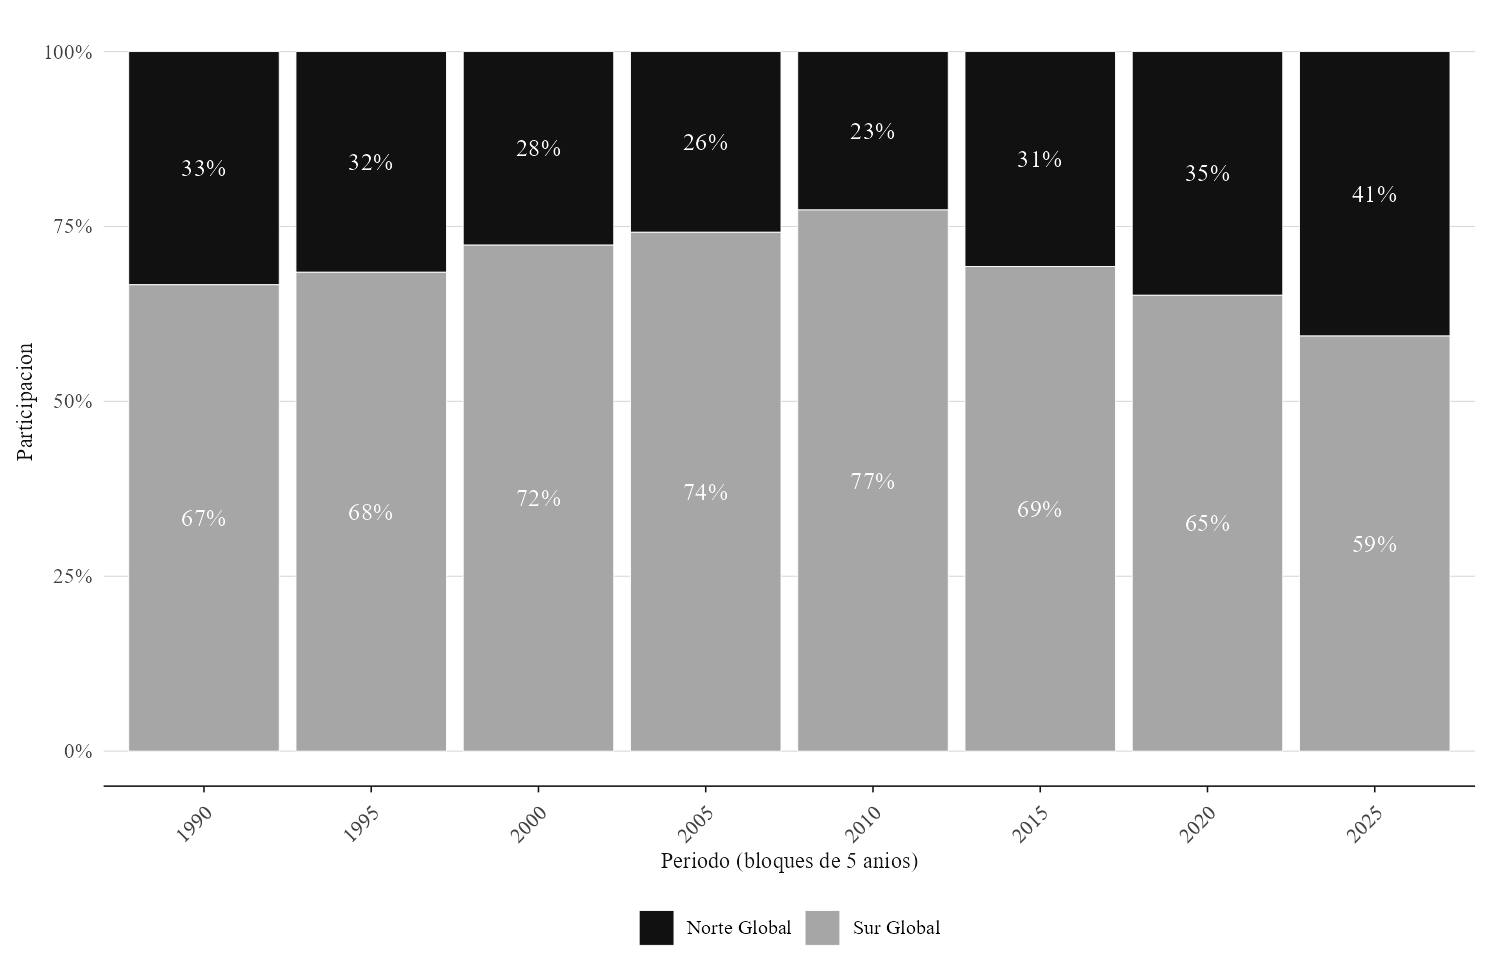
\includegraphics[width=0.85\textwidth]{../08_ANALISIS_R/outputs/20a_norte_sur_global_por_periodo.png}
  \caption{Participaci\'on de los viajes presidenciales sudamericanos dirigidos al Norte Global vs. al Sur Global, por per\'iodo (bloques de 5 a\~nos; mismo formato que la Figura~\ref{fig:categoria-anio}).}
  \label{fig:norte-sur-global-periodo}
\end{figure}

\begin{figure}[H]
  \centering
  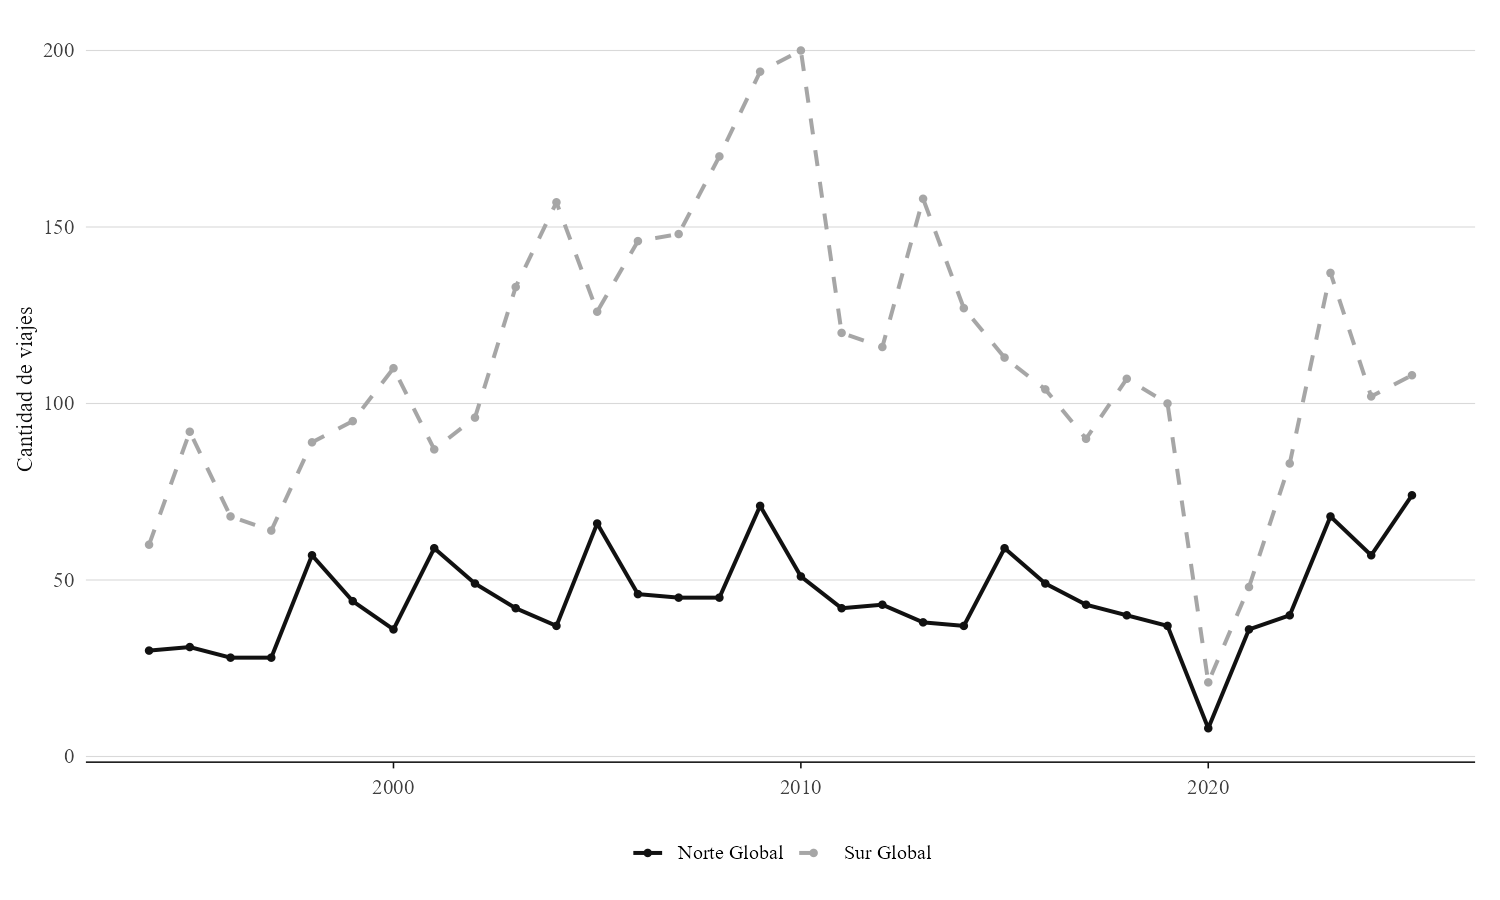
\includegraphics[width=0.85\textwidth]{../08_ANALISIS_R/outputs/20b_norte_sur_global_absoluto.png}
  \caption{Cantidad absoluta de viajes al Norte Global vs. al Sur Global, por a\~no.}
  \label{fig:norte-sur-global-absoluto}
\end{figure}

\begin{figure}[H]
  \centering
  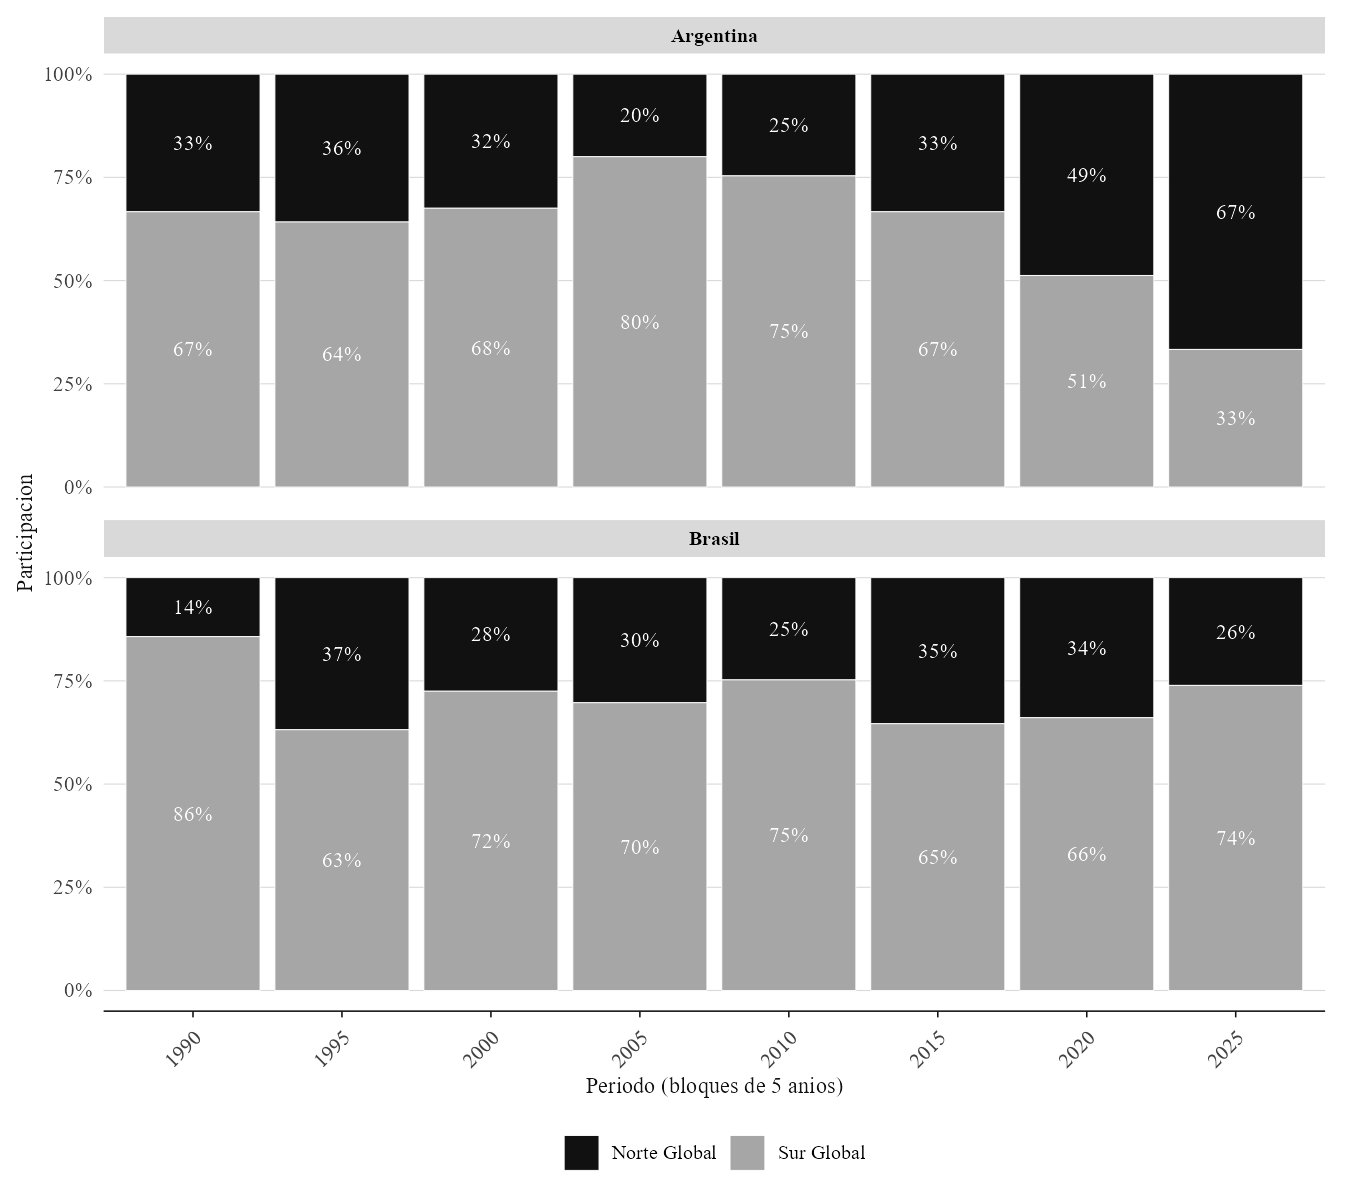
\includegraphics[width=0.8\textwidth]{../08_ANALISIS_R/outputs/20c_norte_sur_global_argentina_brasil.png}
  \caption{Panel especial Argentina/Brasil: participaci\'on de sus viajes dirigidos al Norte Global vs. al Sur Global, por per\'iodo. Permite ver si estos dos pa\'ises -candidatos m\'as plausibles a comportarse ``como Norte Global'' dentro de Sudam\'erica- efectivamente se diferencian del patr\'on regional agregado de la Figura~\ref{fig:norte-sur-global-periodo}.}
  \label{fig:norte-sur-global-arg-bra}
\end{figure}

\subsection{Situaci\'on particular de los mandatarios}
% Area 2: comparaciones a nivel pais/mandato individual -cuanto viaja cada
% pais en promedio por a\~no, a que destinos, con que frecuencia se repiten,
% que tan concentrados estan los rankings de destinos-.

\subsubsection{Promedio de viajes por a\~no, Bilateral y Multilateral, por pa\'is}

% NUEVO (2026-09-11, pedido del usuario, punto 4 del pivot "Diplomacia
% Presidencial"): primero la media anual de viajes de cada pais sudamericano
% (ya usada como linea de referencia en la Figura~\ref{fig:viajes-por-anio-pais}),
% ahora presentada como Cuadro y despues segmentada en Bilateral/Multilateral
% (se excluyen Other y Sin dato de la segmentacion). Ver
% 08_ANALISIS_R/graficos_exploratorios.R, seccion 21, para el detalle.

% latex table generated in R 4.5.1 by xtable 1.8-8 package
% Fri Sep 11 10:51:23 2026
\begin{table}[ht]
\centering
\caption{Promedio de viajes por a\~no, por pa\'is: Bilateral, Multilateral y Total (todas las categor\'ias), 1994-2025.} 
\label{tab:promedio-bilateral-multilateral}
\begin{tabular}{lrrr}
  \hline
Pais & Promedio\_Bilateral & Promedio\_Multilateral & Promedio\_Total \\ 
  \hline
Argentina & 6.41 & 6.16 & 14.91 \\ 
  Bolivia & 3.50 & 6.91 & 13.62 \\ 
  Brasil & 9.41 & 8.06 & 19.28 \\ 
  Chile & 7.56 & 6.69 & 15.72 \\ 
  Colombia & 7.09 & 6.38 & 15.50 \\ 
  Ecuador & 4.03 & 5.78 & 13.50 \\ 
  Guyana & 1.81 & 5.84 & 10.00 \\ 
  Paraguay & 4.16 & 5.91 & 13.28 \\ 
  Peru & 4.34 & 4.25 & 10.42 \\ 
  Surinam & 0.59 & 3.31 & 4.93 \\ 
  Uruguay & 3.69 & 4.25 & 10.81 \\ 
  Venezuela & 8.50 & 4.56 & 16.19 \\ 
   \hline
\end{tabular}
\end{table}
\begin{figure}[H]
  \centering
  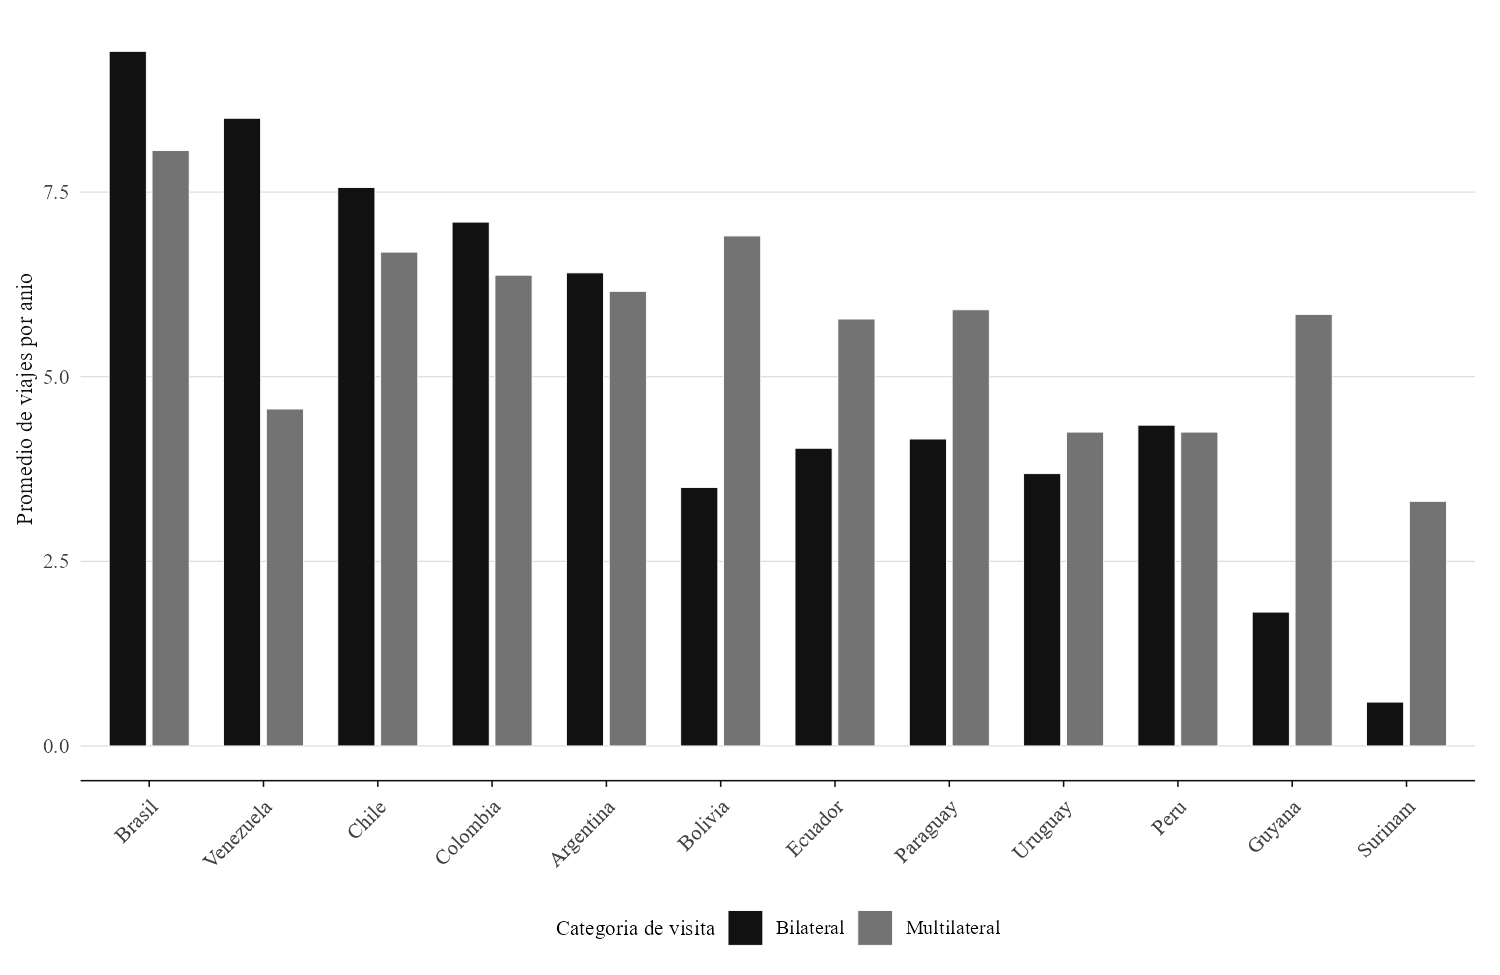
\includegraphics[width=0.9\textwidth]{../08_ANALISIS_R/outputs/21b_promedio_anual_bilateral_multilateral_por_pais.png}
  \caption{Promedio de viajes por a\~no, Bilateral vs. Multilateral, por pa\'is (ordenado de mayor a menor promedio total).}
  \label{fig:promedio-bilateral-multilateral}
\end{figure}

\subsubsection{Comparaci\'on entre pa\'ises}

% El destino favorito por presidente pasa del grafico facetado de 90+
% paneles (dificil de leer) a un Cuadro largo (longtable, pagina a pagina)
% con el pais, el mandatario y su periodo entre parentesis, el destino
% favorito y la cantidad de viajes a ese destino.
%
% Metodologia (pedido del usuario, decisiones documentadas explicitamente):
%  (1) Se separa por MANDATO INDIVIDUAL, no por presidente completo -un
%      presidente reelecto (ej. Cristina Fernandez de Kirchner, 2007-2011 y
%      2011-2015) aparece en 2 filas independientes, para poder comparar si
%      el destino favorito se mantuvo entre un mandato y el siguiente.
%  (2) El "destino favorito" se calcula SOLO sobre viajes BILATERALES (no
%      sobre el total), para que un pais que acumula visitas por ser sede
%      recurrente de cumbres multilaterales no distorsione el resultado.
%  (3) Regla de desempate cuando 2 o mas paises quedan empatados en el
%      maximo de viajes bilaterales dentro de un mismo mandato: se
%      prioriza el pais que ALCANZO ese conteo maximo PRIMERO en el tiempo
%      (fecha del viaje N-esimo mas temprana).
% latex table generated in R 4.5.1 by xtable 1.8-8 package
% Fri Sep 11 10:51:23 2026
\begingroup\footnotesize
\begin{longtable}{lllr}
\caption{Destino favorito BILATERAL de cada mandato individual (pa\'is m\'as visitado en viajes bilaterales durante ese mandato espec\'ifico), con el mandato entre par\'entesis. Desempates: prioridad al pa\'is que alcanz\'o el conteo m\'aximo primero en el tiempo.} \\ 
  \hline
Pais & Mandatario..mandato. & Destino.favorito..bilateral. & Cantidad.de.viajes \\ 
  \hline
Argentina & Carlos Saul Menem (1994-1995) & Mexico &   1 \\ 
  Argentina & Carlos Saul Menem (1995-1999) & Brazil &   3 \\ 
  Argentina & Fernando de la Rua (1999-2001) & United States &   2 \\ 
  Argentina & Eduardo Duhalde (2002-2003) & Brazil &   2 \\ 
  Argentina & Nestor Kirchner (2003-2007) & Spain &   4 \\ 
  Argentina & Cristina Fernandez de Kirchner (2007-2011) & Venezuela &   5 \\ 
  Argentina & Cristina Fernandez de Kirchner (2011-2015) & Holy See &   4 \\ 
  Argentina & Mauricio Macri (2015-2019) & Holy See &   2 \\ 
  Argentina & Alberto Fernandez (2019-2023) & Spain &   3 \\ 
  Argentina & Javier Milei (2023-2025) & Italy &   4 \\ 
  Bolivia & Gonzalo Sanchez de Lozada (1994-1997) & Argentina &   3 \\ 
  Bolivia & Hugo Banzer Suarez (1997-2001) & Italy &   1 \\ 
  Bolivia & Gonzalo Sanchez de Lozada (2002-2003) & Brazil &   2 \\ 
  Bolivia & Carlos Mesa (2003-2005) & Brazil &   1 \\ 
  Bolivia & Evo Morales (2006-2010) & Venezuela &   3 \\ 
  Bolivia & Evo Morales (2010-2015) & Venezuela &   4 \\ 
  Bolivia & Evo Morales (2015-2019) & Cuba &   3 \\ 
  Bolivia & Luis Arce (2020-2025) & Venezuela &   2 \\ 
  Brasil & Itamar Franco (1994-1995) & Colombia &   1 \\ 
  Brasil & Fernando Henrique Cardoso (1995-1999) & United Kingdom &   3 \\ 
  Brasil & Fernando Henrique Cardoso (1999-2003) & Germany &   3 \\ 
  Brasil & Luiz Inacio Lula da Silva (2003-2007) & Guyana &   3 \\ 
  Brasil & Luiz Inacio Lula da Silva (2007-2011) & Venezuela &   5 \\ 
  Brasil & Dilma Rousseff (2011-2015) & Argentina &   4 \\ 
  Brasil & Dilma Rousseff (2015-2016) & Bolivia &   2 \\ 
  Brasil & Michel Temer (2016-2019) & Paraguay &   2 \\ 
  Brasil & Jair Bolsonaro (2019-2023) & Israel &   2 \\ 
  Brasil & Luiz Inacio Lula da Silva (2023-2025) & Uruguay &   3 \\ 
  Chile & Eduardo Frei Ruiz-Tagle (1994-2000) & Argentina &   4 \\ 
  Chile & Ricardo Lagos Escobar (2000-2006) & Argentina &   4 \\ 
  Chile & Michelle Bachelet (2006-2010) & Argentina &   3 \\ 
  Chile & Sebastian Pinera (2010-2014) & Argentina &   3 \\ 
  Chile & Michelle Bachelet (2014-2018) & Uruguay &   2 \\ 
  Chile & Sebastian Pinera (2018-2022) & Brazil &   3 \\ 
  Chile & Gabriel Boric (2022-2026) & Mexico &   2 \\ 
  Colombia & Cesar Gaviria Trujillo (1994-1994) & Japan &   1 \\ 
  Colombia & Ernesto Samper Pizano (1994-1998) & France &   1 \\ 
  Colombia & Andres Pastrana Arango (1998-2002) & United States &   4 \\ 
  Colombia & Alvaro Uribe (2002-2006) & United States &   6 \\ 
  Colombia & Alvaro Uribe (2006-2010) & United States &   4 \\ 
  Colombia & Juan Manuel Santos (2010-2014) & Brazil &   3 \\ 
  Colombia & Juan Manuel Santos (2014-2018) & Spain &   4 \\ 
  Colombia & Ivan Duque (2018-2022) & Ecuador &   4 \\ 
  Colombia & Gustavo Petro (2022-2026) & Venezuela &   5 \\ 
  Ecuador & Sixto Duran-Ballen (1994-1996) & Japan &   1 \\ 
  Ecuador & Abdala Bucaram (1996-1997) & Peru &   1 \\ 
  Ecuador & Fabian Alarcon (1997-1998) & Peru &   1 \\ 
  Ecuador & Jamil Mahuad (1998-2000) & Peru &   2 \\ 
  Ecuador & Gustavo Noboa (2000-2003) & Colombia &   1 \\ 
  Ecuador & Lucio Gutierrez (2003-2005) & United States &   1 \\ 
  Ecuador & Alfredo Palacio (2005-2007) & Colombia &   1 \\ 
  Ecuador & Rafael Correa (2007-2009) & Brazil &   3 \\ 
  Ecuador & Rafael Correa (2009-2013) & Colombia &   3 \\ 
  Ecuador & Rafael Correa (2013-2017) & Colombia &   2 \\ 
  Ecuador & Lenin Moreno (2017-2021) & Colombia &   2 \\ 
  Ecuador & Guillermo Lasso (2021-2023) & Colombia &   4 \\ 
  Ecuador & Daniel Noboa (2023-2025) & United States &   2 \\ 
  Ecuador & Daniel Noboa (2025-2025) & Italy &   1 \\ 
  Guyana & Cheddi Jagan (1994-1997) & Colombia &   1 \\ 
  Guyana & Janet Jagan (1997-1999) & Venezuela &   1 \\ 
  Guyana & Bharrat Jagdeo (1999-2001) & Jamaica &   1 \\ 
  Guyana & Bharrat Jagdeo (2001-2006) & United Kingdom &   3 \\ 
  Guyana & Bharrat Jagdeo (2006-2011) & Russia &   2 \\ 
  Guyana & Donald Ramotar (2011-2015) & Suriname &   1 \\ 
  Guyana & David Granger (2015-2020) & Trinidad and Tobago &   1 \\ 
  Guyana & Irfaan Ali (2020-2025) & Barbados &   2 \\ 
  Paraguay & Juan Carlos Wasmosy (1994-1998) & Brazil &   5 \\ 
  Paraguay & Raul Cubas Grau (1998-1999) & Brazil &   1 \\ 
  Paraguay & Luis Angel Gonzalez Macchi (1999-2003) & Brazil &   1 \\ 
  Paraguay & Nicanor Duarte (2003-2008) & Taiwan &   2 \\ 
  Paraguay & Fernando Lugo (2008-2012) & Brazil &   3 \\ 
  Paraguay & Federico Franco (2012-2013) & Taiwan &   1 \\ 
  Paraguay & Horacio Cartes (2013-2018) & Argentina &   4 \\ 
  Paraguay & Mario Abdo Benitez (2018-2023) & Brazil &   5 \\ 
  Paraguay & Santiago Pena (2023-2025) & Argentina &   3 \\ 
  Peru & Alberto Fujimori (1994-1995) & Colombia &   2 \\ 
  Peru & Alberto Fujimori (1995-2000) & Brazil &   6 \\ 
  Peru & Alejandro Toledo (2001-2006) & Ecuador &   2 \\ 
  Peru & Alan Garcia (2006-2011) & United States &   4 \\ 
  Peru & Ollanta Humala (2011-2016) & Spain &   3 \\ 
  Peru & Pedro Pablo Kuczynski (2016-2018) & China &   1 \\ 
  Peru & Martin Vizcarra (2018-2020) & Bolivia &   2 \\ 
  Peru & Pedro Castillo (2021-2022) & Chile &   2 \\ 
  Peru & Dina Boluarte (2022-2025) & Holy See &   2 \\ 
  Peru & Jose Jeri (2025-2026) & Ecuador &   1 \\ 
  Surinam & Ronald Venetiaan (1994-1996) & Indonesia &   1 \\ 
  Surinam & Jules Wijdenbosch (1996-2000) & China &   1 \\ 
  Surinam & Ronald Venetiaan (2000-2010) & Netherlands &   1 \\ 
  Surinam & Desi Bouterse (2010-2015) & Guyana &   1 \\ 
  Surinam & Desi Bouterse (2015-2020) & Brazil &   1 \\ 
  Surinam & Chandrikapersad Santokhi (2020-2025) & Guyana &   3 \\ 
  Surinam & Jennifer Geerlings-Simons (2025-2025) & Netherlands &   1 \\ 
  Uruguay & Luis Alberto Lacalle (1994-1995) & Brazil &   1 \\ 
  Uruguay & Julio Maria Sanguinetti (1995-2000) & Egypt &   2 \\ 
  Uruguay & Jorge Batlle (2000-2005) & United States &   2 \\ 
  Uruguay & Tabare Vazquez (2005-2010) & Brazil &   4 \\ 
  Uruguay & Jose Mujica (2010-2015) & Argentina &   6 \\ 
  Uruguay & Tabare Vazquez (2015-2020) & Argentina &   3 \\ 
  Uruguay & Luis Lacalle Pou (2020-2025) & Paraguay &   2 \\ 
  Uruguay & Yamandu Orsi (2025-2025) & Panama &   1 \\ 
  Venezuela & Rafael Caldera (1994-1999) & Brazil &   2 \\ 
  Venezuela & Hugo Chavez (1999-2000) & China &   2 \\ 
  Venezuela & Hugo Chavez (2000-2007) & Cuba &  10 \\ 
  Venezuela & Hugo Chavez (2007-2013) & Cuba &  22 \\ 
  Venezuela & Nicolas Maduro (2013-2019) & Cuba &   5 \\ 
  Venezuela & Nicolas Maduro (2019-2025) & Russia &   2 \\ 
   \hline
\hline
\label{tab:destino-favorito}
\end{longtable}
\endgroup
\begin{figure}[H]
  \centering
  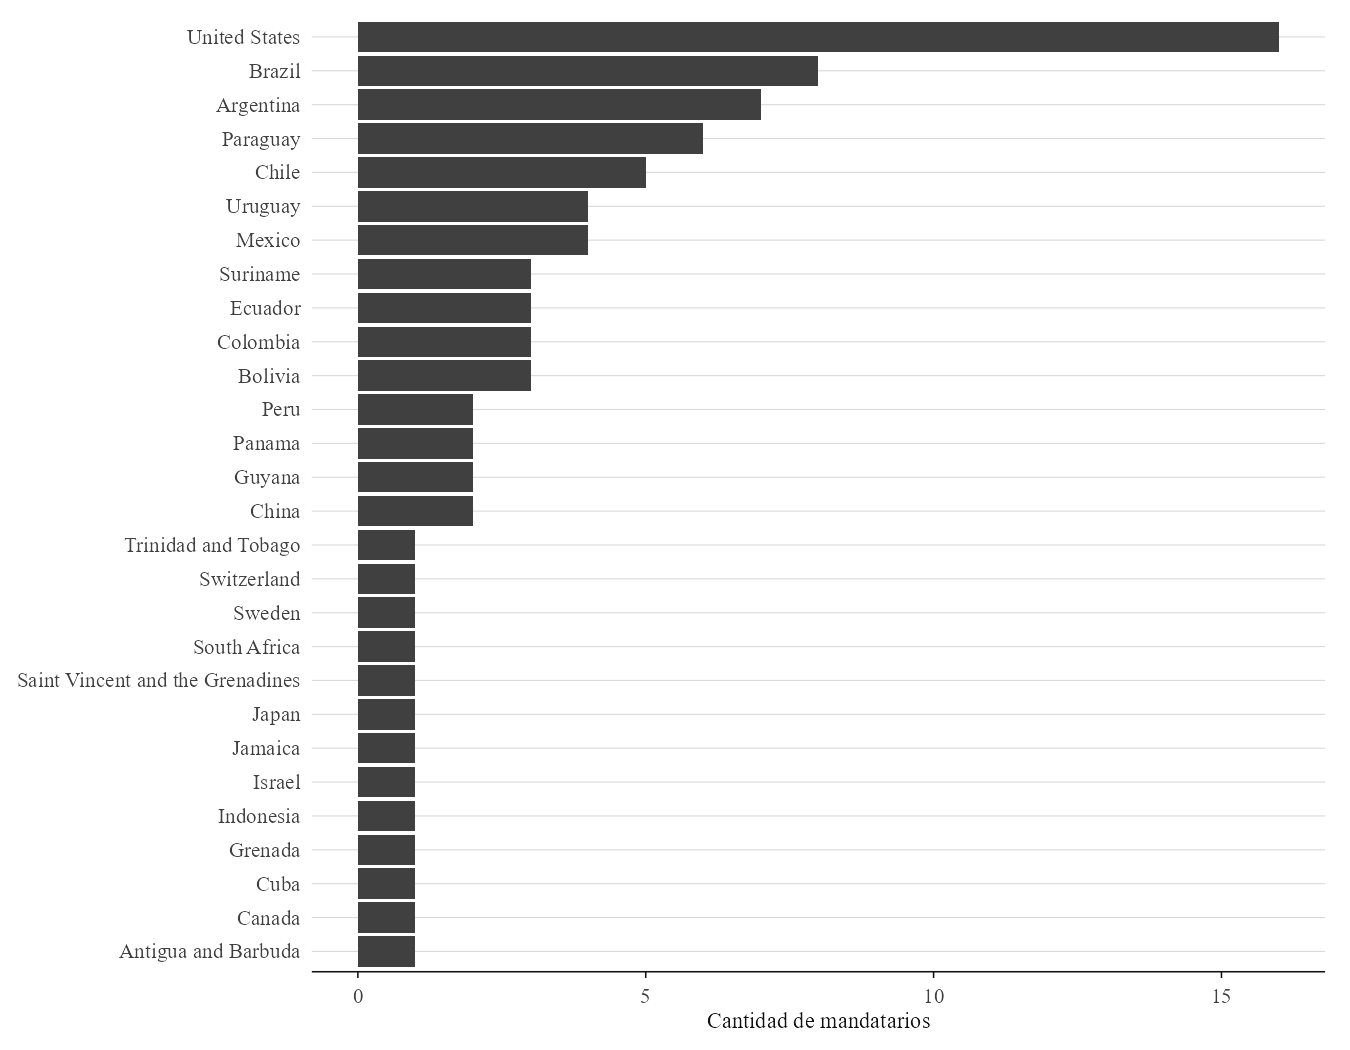
\includegraphics[width=0.85\textwidth]{../08_ANALISIS_R/outputs/06_primeros_destinos_frecuencia.png}
  \caption{Pa\'is elegido como primer viaje al exterior del mandato, cu\'antas veces se repite cada uno (ver \citep{ostranderPresidentsAbroadPolitics2018}, Tabla 1, para el equivalente en EE.\,UU.).}
  \label{fig:primeros-destinos}
\end{figure}

% ELIMINADA (2026-09-10, pedido del usuario, item 10): figura de evolucion
% anual de primer-destino para Estados Unidos/Brasil/Argentina
% (06b_evolucion_top3_primeros_destinos.png). Se reemplaza por la variante
% de abajo, restringida a solo viajes BILATERALES (item 9).

\begin{figure}[H]
  \centering
  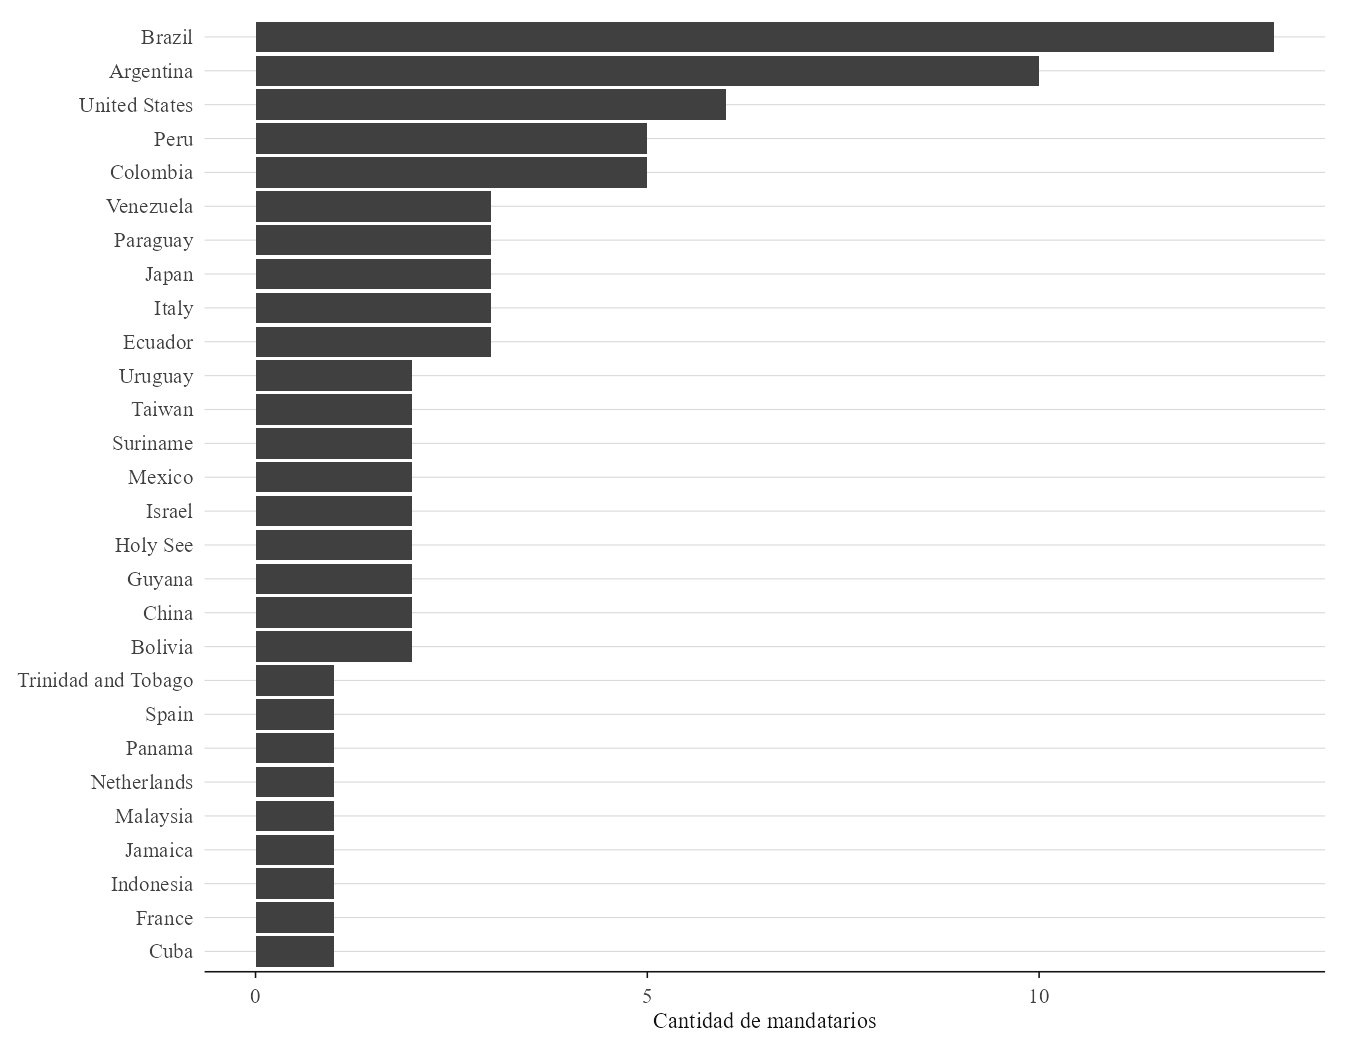
\includegraphics[width=0.85\textwidth]{../08_ANALISIS_R/outputs/06c_primeros_destinos_frecuencia_bilateral.png}
  \caption{Igual que la Figura~\ref{fig:primeros-destinos}, pero contando solo el primer viaje de categor\'ia BILATERAL de cada mandatario (no su primer viaje de cualquier categor\'ia). Responde una pregunta m\'as espec\'ifica: no ``a qu\'e pa\'is viaj\'o primero'' sino ``a qu\'e pa\'is hizo su primera visita bilateral a otro Jefe de Estado''.}
  \label{fig:primeros-destinos-bilateral}
\end{figure}

% NOTA (2026-09-11, pedido del usuario, pivot "Diplomacia Presidencial"): el
% bloque de "sesgo hacia el vecino inmediato" (Figura sesgo-vecino-inmediato,
% Cuadro correlacion-vecino, Figura vecino-a-lo-largo-del-tiempo) se MOVIO al
% Area 3 ("Mandatarios, ideolog\'ia, cercan\'ia y comercio"), subsecci\'on
% "Cercan\'ia geogr\'afica", junto con Ideolog\'ia y Homofilia -las 3
% dimensiones que el usuario pidio agrupar para explicar el comportamiento
% individual de cada mandatario-. Ver mas abajo, despues de la Figura de
% composici\'on por pa\'is.

% Cuadro complementario: el "perfil" de cada MANDATO (no de cada presidente
% completo) resumido en todo ese mandato (a diferencia de la Figura
% anterior, que agrega por pais de origen). Categorias mutuamente
% excluyentes (a diferencia de la Figura~\ref{fig:evolucion-por-bloque-destino},
% que las deja superpuestas a proposito) para que cada fila sume 100%.
% Metodologia (pedido del usuario): separado por mandato individual (mismo
% criterio que el Cuadro~\ref{tab:destino-favorito}); los mandatos en curso
% (marcados internamente con el placeholder 2099) se muestran como 2025;
% orden alfabetico por pais y, DENTRO de cada pais, cronologico por inicio
% de mandato (ej. Argentina: Menem 1 y 2 primero, Milei ultimo -no
% alfabetico por nombre de mandatario-).
% Nota tecnica (2026-09-06, v3 -la v1 con pdflscape fallo por no tener ese
% paquete instalado, "File pdflscape.sty not found"; la v2 uso solamente
% \newgeometry{paperwidth=..., paperheight=...} del paquete "geometry", pero
% se comprobo empiricamente -renderizando las paginas del PDF compilado a
% PNG y comparando dimensiones en pixeles- que el tama\~no de pagina real
% NUNCA cambiaba: todas las paginas salian A4 vertical estandar pese a la
% directiva. geometry ajusta los margenes/layout de LaTeX pero no siempre
% logra mover el media box real que pdfTeX efectivamente usa al hacer
% \shipout de cada pagina, sobre todo en medio de un documento con una
% longtable que genera sus propios saltos de pagina internos-): esta version
% fuerza el tama\~no de pagina con las primitivas nativas de pdfTeX
% (\pdfpagewidth/\pdfpageheight), que son las que pdfTeX realmente consulta
% al momento de cada \shipout, ademas de \newgeometry (para que los margenes
% se recalculen de forma consistente). Con 8 columnas de region + Pais +
% Mandatario + Total viajes (11 columnas en total) la tabla no entraba ni en
% vertical con margenes de 1cm y fuente tiny -quedaba desbordada y
% descentrada-; en apaisado (29.7x21cm) hay bastante mas ancho util (~26.7cm
% vs ~19cm en vertical con margen de 1cm) y el texto queda derecho -no hay
% que girar nada para leerlo, la pagina simplemente es mas ancha que alta en
% esa seccion del PDF-.
\clearpage
\pdfpagewidth=29.7cm
\pdfpageheight=21cm
\newgeometry{paperwidth=29.7cm, paperheight=21cm, margin=1.5cm}
% latex table generated in R 4.5.1 by xtable 1.8-8 package
% Fri Sep 11 10:51:23 2026
\begingroup\tiny
\begin{longtable}{lllllllllll}
\caption{Perfil regional de cada MANDATO individual: porcentaje de sus viajes a cada bloque de destino. Las categor\'ias son mutuamente excluyentes y suman 100\% por fila. Para mandatos iniciados antes de 1994 (ej. primer mandato de Menem, Fujimori, S\'anchez de Lozada, entre otros), el a\~no de inicio mostrado es 1994, ya que nuestra base solo tiene cobertura verificada desde esa fecha -el mandato real empez\'o antes, pero solo se cuentan los viajes a partir de 1994. Los mandatos marcados con * tienen cobertura PARCIAL en nuestra base: arrancaron antes de 1994 y/o siguen en curso a la fecha de corte (septiembre de 2026), por lo que su perfil regional no refleja necesariamente el mandato completo.} \\ 
  \hline
Pais & Mandatario..mandato. & Total.viajes & Sudamerica & Resto.Latam.y.Caribe & Estados.Unidos & Resto.Norteamerica & Europa & Asia & Africa & Otras..Oceania..etc.. \\ 
  \hline
Argentina & Carlos Saul Menem (1994-1995)* & 7 & 43\% & 14\% & 14\% & 0\% & 14\% & 0\% & 14\% & 0\% \\ 
  Argentina & Carlos Saul Menem (1995-1999) & 77 & 29\% & 10\% & 16\% & 0\% & 27\% & 14\% & 1\% & 3\% \\ 
  Argentina & Fernando de la Rua (1999-2001) & 35 & 46\% & 11\% & 11\% & 6\% & 23\% & 3\% & 0\% & 0\% \\ 
  Argentina & Eduardo Duhalde (2002-2003) & 17 & 47\% & 18\% & 0\% & 0\% & 29\% & 0\% & 6\% & 0\% \\ 
  Argentina & Nestor Kirchner (2003-2007) & 59 & 61\% & 5\% & 12\% & 0\% & 20\% & 2\% & 0\% & 0\% \\ 
  Argentina & Cristina Fernandez de Kirchner (2007-2011) & 76 & 47\% & 11\% & 8\% & 3\% & 17\% & 9\% & 5\% & 0\% \\ 
  Argentina & Cristina Fernandez de Kirchner (2011-2015) & 48 & 50\% & 10\% & 12\% & 0\% & 17\% & 8\% & 2\% & 0\% \\ 
  Argentina & Mauricio Macri (2015-2019) & 57 & 35\% & 0\% & 14\% & 2\% & 28\% & 19\% & 2\% & 0\% \\ 
  Argentina & Alberto Fernandez (2019-2023) & 55 & 38\% & 7\% & 7\% & 0\% & 38\% & 9\% & 0\% & 0\% \\ 
  Argentina & Javier Milei (2023-2025)* & 46 & 20\% & 2\% & 30\% & 0\% & 43\% & 4\% & 0\% & 0\% \\ 
  Bolivia & Gonzalo Sanchez de Lozada (1994-1997)* & 34 & 53\% & 3\% & 18\% & 0\% & 24\% & 3\% & 0\% & 0\% \\ 
  Bolivia & Hugo Banzer Suarez (1997-2001) & 24 & 58\% & 12\% & 12\% & 4\% & 12\% & 0\% & 0\% & 0\% \\ 
  Bolivia & Jorge Quiroga Ramirez (2001-2002) & 6 & 67\% & 0\% & 17\% & 0\% & 17\% & 0\% & 0\% & 0\% \\ 
  Bolivia & Gonzalo Sanchez de Lozada (2002-2003) & 12 & 58\% & 17\% & 17\% & 0\% & 8\% & 0\% & 0\% & 0\% \\ 
  Bolivia & Carlos Mesa (2003-2005) & 20 & 55\% & 20\% & 5\% & 0\% & 15\% & 5\% & 0\% & 0\% \\ 
  Bolivia & Eduardo Rodriguez (2005-2006) & 6 & 67\% & 0\% & 17\% & 0\% & 17\% & 0\% & 0\% & 0\% \\ 
  Bolivia & Evo Morales (2006-2010) & 87 & 56\% & 18\% & 8\% & 0\% & 11\% & 3\% & 2\% & 0\% \\ 
  Bolivia & Evo Morales (2010-2015) & 108 & 54\% & 10\% & 8\% & 0\% & 19\% & 6\% & 3\% & 1\% \\ 
  Bolivia & Evo Morales (2015-2019) & 90 & 36\% & 21\% & 11\% & 0\% & 28\% & 4\% & 0\% & 0\% \\ 
  Bolivia & Luis Arce (2020-2025) & 49 & 55\% & 22\% & 10\% & 0\% & 8\% & 0\% & 4\% & 0\% \\ 
  Brasil & Itamar Franco (1994-1995)* & 7 & 86\% & 0\% & 14\% & 0\% & 0\% & 0\% & 0\% & 0\% \\ 
  Brasil & Fernando Henrique Cardoso (1995-1999) & 60 & 45\% & 2\% & 8\% & 2\% & 32\% & 8\% & 3\% & 0\% \\ 
  Brasil & Fernando Henrique Cardoso (1999-2003) & 74 & 36\% & 15\% & 7\% & 1\% & 32\% & 4\% & 4\% & 0\% \\ 
  Brasil & Luiz Inacio Lula da Silva (2003-2007) & 115 & 42\% & 7\% & 6\% & 0\% & 21\% & 6\% & 18\% & 0\% \\ 
  Brasil & Luiz Inacio Lula da Silva (2007-2011) & 151 & 34\% & 13\% & 5\% & 0\% & 27\% & 13\% & 9\% & 0\% \\ 
  Brasil & Dilma Rousseff (2011-2015) & 66 & 38\% & 8\% & 8\% & 0\% & 27\% & 6\% & 12\% & 2\% \\ 
  Brasil & Dilma Rousseff (2015-2016) & 21 & 38\% & 14\% & 14\% & 0\% & 29\% & 5\% & 0\% & 0\% \\ 
  Brasil & Michel Temer (2016-2019) & 26 & 35\% & 8\% & 12\% & 0\% & 19\% & 15\% & 12\% & 0\% \\ 
  Brasil & Jair Bolsonaro (2019-2023) & 34 & 21\% & 0\% & 21\% & 0\% & 18\% & 41\% & 0\% & 0\% \\ 
  Brasil & Luiz Inacio Lula da Silva (2023-2025)* & 63 & 27\% & 6\% & 6\% & 2\% & 27\% & 19\% & 13\% & 0\% \\ 
  Chile & Eduardo Frei Ruiz-Tagle (1994-2000) & 64 & 41\% & 8\% & 8\% & 3\% & 19\% & 17\% & 2\% & 3\% \\ 
  Chile & Ricardo Lagos Escobar (2000-2006) & 135 & 36\% & 17\% & 7\% & 1\% & 25\% & 10\% & 1\% & 2\% \\ 
  Chile & Michelle Bachelet (2006-2010) & 80 & 35\% & 22\% & 9\% & 1\% & 20\% & 10\% & 0\% & 2\% \\ 
  Chile & Sebastian Pinera (2010-2014) & 64 & 39\% & 8\% & 9\% & 2\% & 22\% & 19\% & 0\% & 2\% \\ 
  Chile & Michelle Bachelet (2014-2018) & 59 & 31\% & 20\% & 12\% & 2\% & 20\% & 10\% & 5\% & 0\% \\ 
  Chile & Sebastian Pinera (2018-2022) & 48 & 44\% & 8\% & 6\% & 0\% & 25\% & 12\% & 0\% & 4\% \\ 
  Chile & Gabriel Boric (2022-2026) & 53 & 40\% & 9\% & 13\% & 2\% & 23\% & 13\% & 0\% & 0\% \\ 
  Colombia & Cesar Gaviria Trujillo (1994-1994)* & 2 & 50\% & 0\% & 0\% & 0\% & 0\% & 50\% & 0\% & 0\% \\ 
  Colombia & Ernesto Samper Pizano (1994-1998) & 27 & 30\% & 4\% & 15\% & 4\% & 11\% & 22\% & 15\% & 0\% \\ 
  Colombia & Andres Pastrana Arango (1998-2002) & 53 & 26\% & 17\% & 19\% & 4\% & 23\% & 8\% & 4\% & 0\% \\ 
  Colombia & Alvaro Uribe (2002-2006) & 66 & 44\% & 24\% & 17\% & 0\% & 12\% & 3\% & 0\% & 0\% \\ 
  Colombia & Alvaro Uribe (2006-2010) & 71 & 39\% & 30\% & 17\% & 3\% & 11\% & 0\% & 0\% & 0\% \\ 
  Colombia & Juan Manuel Santos (2010-2014) & 70 & 34\% & 24\% & 11\% & 1\% & 17\% & 11\% & 0\% & 0\% \\ 
  Colombia & Juan Manuel Santos (2014-2018) & 81 & 22\% & 19\% & 14\% & 1\% & 42\% & 2\% & 0\% & 0\% \\ 
  Colombia & Ivan Duque (2018-2022) & 52 & 31\% & 17\% & 19\% & 0\% & 25\% & 8\% & 0\% & 0\% \\ 
  Colombia & Gustavo Petro (2022-2026) & 74 & 32\% & 22\% & 12\% & 0\% & 20\% & 11\% & 3\% & 0\% \\ 
  Ecuador & Sixto Duran-Ballen (1994-1996)* & 16 & 75\% & 0\% & 6\% & 0\% & 12\% & 6\% & 0\% & 0\% \\ 
  Ecuador & Abdala Bucaram (1996-1997) & 4 & 100\% & 0\% & 0\% & 0\% & 0\% & 0\% & 0\% & 0\% \\ 
  Ecuador & Fabian Alarcon (1997-1998) & 9 & 67\% & 0\% & 22\% & 11\% & 0\% & 0\% & 0\% & 0\% \\ 
  Ecuador & Jamil Mahuad (1998-2000) & 21 & 43\% & 19\% & 29\% & 0\% & 5\% & 5\% & 0\% & 0\% \\ 
  Ecuador & Gustavo Noboa (2000-2003) & 31 & 45\% & 13\% & 10\% & 6\% & 13\% & 10\% & 3\% & 0\% \\ 
  Ecuador & Lucio Gutierrez (2003-2005) & 22 & 45\% & 18\% & 23\% & 0\% & 9\% & 5\% & 0\% & 0\% \\ 
  Ecuador & Alfredo Palacio (2005-2007) & 20 & 50\% & 20\% & 10\% & 0\% & 15\% & 0\% & 5\% & 0\% \\ 
  Ecuador & Rafael Correa (2007-2009) & 54 & 50\% & 22\% & 4\% & 0\% & 15\% & 9\% & 0\% & 0\% \\ 
  Ecuador & Rafael Correa (2009-2013) & 77 & 53\% & 17\% & 3\% & 1\% & 22\% & 4\% & 0\% & 0\% \\ 
  Ecuador & Rafael Correa (2013-2017) & 59 & 39\% & 19\% & 7\% & 0\% & 29\% & 5\% & 2\% & 0\% \\ 
  Ecuador & Lenin Moreno (2017-2021) & 35 & 31\% & 9\% & 23\% & 0\% & 29\% & 9\% & 0\% & 0\% \\ 
  Ecuador & Guillermo Lasso (2021-2023) & 36 & 36\% & 14\% & 25\% & 0\% & 19\% & 6\% & 0\% & 0\% \\ 
  Ecuador & Daniel Noboa (2023-2025) & 33 & 12\% & 6\% & 33\% & 3\% & 39\% & 6\% & 0\% & 0\% \\ 
  Ecuador & Daniel Noboa (2025-2025)* & 15 & 27\% & 0\% & 27\% & 0\% & 27\% & 20\% & 0\% & 0\% \\ 
  Guyana & Cheddi Jagan (1994-1997)* & 24 & 12\% & 42\% & 12\% & 4\% & 8\% & 12\% & 4\% & 4\% \\ 
  Guyana & Janet Jagan (1997-1999) & 14 & 50\% & 29\% & 14\% & 0\% & 7\% & 0\% & 0\% & 0\% \\ 
  Guyana & Bharrat Jagdeo (1999-2001) & 8 & 12\% & 75\% & 12\% & 0\% & 0\% & 0\% & 0\% & 0\% \\ 
  Guyana & Bharrat Jagdeo (2001-2006) & 60 & 18\% & 35\% & 23\% & 3\% & 12\% & 5\% & 2\% & 2\% \\ 
  Guyana & Bharrat Jagdeo (2006-2011) & 80 & 15\% & 29\% & 19\% & 0\% & 16\% & 16\% & 5\% & 0\% \\ 
  Guyana & Donald Ramotar (2011-2015) & 34 & 35\% & 38\% & 12\% & 0\% & 0\% & 12\% & 3\% & 0\% \\ 
  Guyana & David Granger (2015-2020) & 48 & 15\% & 44\% & 19\% & 0\% & 10\% & 8\% & 4\% & 0\% \\ 
  Guyana & Irfaan Ali (2020-2025)* & 52 & 12\% & 35\% & 23\% & 4\% & 10\% & 15\% & 0\% & 2\% \\ 
  Paraguay & Juan Carlos Wasmosy (1994-1998)* & 57 & 65\% & 7\% & 5\% & 0\% & 16\% & 7\% & 0\% & 0\% \\ 
  Paraguay & Raul Cubas Grau (1998-1999) & 4 & 100\% & 0\% & 0\% & 0\% & 0\% & 0\% & 0\% & 0\% \\ 
  Paraguay & Luis Angel Gonzalez Macchi (1999-2003) & 31 & 65\% & 16\% & 6\% & 3\% & 3\% & 6\% & 0\% & 0\% \\ 
  Paraguay & Nicanor Duarte (2003-2008) & 60 & 62\% & 8\% & 7\% & 0\% & 15\% & 7\% & 2\% & 0\% \\ 
  Paraguay & Fernando Lugo (2008-2012) & 76 & 59\% & 14\% & 7\% & 0\% & 7\% & 13\% & 0\% & 0\% \\ 
  Paraguay & Federico Franco (2012-2013) & 6 & 0\% & 0\% & 50\% & 0\% & 17\% & 33\% & 0\% & 0\% \\ 
  Paraguay & Horacio Cartes (2013-2018) & 70 & 51\% & 9\% & 9\% & 0\% & 20\% & 11\% & 0\% & 0\% \\ 
  Paraguay & Mario Abdo Benitez (2018-2023) & 59 & 56\% & 8\% & 12\% & 0\% & 15\% & 8\% & 0\% & 0\% \\ 
  Paraguay & Santiago Pena (2023-2025)* & 62 & 32\% & 11\% & 15\% & 0\% & 26\% & 15\% & 2\% & 0\% \\ 
  Peru & Alberto Fujimori (1994-1995)* & 15 & 67\% & 7\% & 7\% & 0\% & 7\% & 13\% & 0\% & 0\% \\ 
  Peru & Alberto Fujimori (1995-2000) & 77 & 39\% & 9\% & 10\% & 4\% & 12\% & 22\% & 1\% & 3\% \\ 
  Peru & Alberto Fujimori (2000-2000) & 3 & 33\% & 0\% & 67\% & 0\% & 0\% & 0\% & 0\% & 0\% \\ 
  Peru & Alejandro Toledo (2001-2006) & 62 & 42\% & 8\% & 18\% & 0\% & 23\% & 10\% & 0\% & 0\% \\ 
  Peru & Alan Garcia (2006-2011) & 41 & 51\% & 7\% & 10\% & 0\% & 12\% & 17\% & 0\% & 2\% \\ 
  Peru & Ollanta Humala (2011-2016) & 67 & 34\% & 12\% & 9\% & 1\% & 28\% & 15\% & 0\% & 0\% \\ 
  Peru & Pedro Pablo Kuczynski (2016-2018) & 14 & 50\% & 0\% & 14\% & 0\% & 21\% & 14\% & 0\% & 0\% \\ 
  Peru & Martin Vizcarra (2018-2020) & 16 & 50\% & 25\% & 12\% & 0\% & 12\% & 0\% & 0\% & 0\% \\ 
  Peru & Pedro Castillo (2021-2022) & 10 & 60\% & 10\% & 30\% & 0\% & 0\% & 0\% & 0\% & 0\% \\ 
  Peru & Dina Boluarte (2022-2025) & 17 & 18\% & 0\% & 24\% & 0\% & 41\% & 18\% & 0\% & 0\% \\ 
  Peru & Jose Jeri (2025-2026) & 1 & 100\% & 0\% & 0\% & 0\% & 0\% & 0\% & 0\% & 0\% \\ 
  Surinam & Ronald Venetiaan (1994-1996)* & 7 & 14\% & 14\% & 43\% & 0\% & 0\% & 29\% & 0\% & 0\% \\ 
  Surinam & Jules Wijdenbosch (1996-2000) & 16 & 0\% & 81\% & 6\% & 0\% & 0\% & 12\% & 0\% & 0\% \\ 
  Surinam & Ronald Venetiaan (2000-2010) & 33 & 18\% & 58\% & 6\% & 3\% & 6\% & 3\% & 6\% & 0\% \\ 
  Surinam & Desi Bouterse (2010-2015) & 33 & 48\% & 36\% & 6\% & 0\% & 0\% & 3\% & 6\% & 0\% \\ 
  Surinam & Desi Bouterse (2015-2020) & 6 & 33\% & 50\% & 0\% & 0\% & 0\% & 17\% & 0\% & 0\% \\ 
  Surinam & Chandrikapersad Santokhi (2020-2025) & 45 & 20\% & 36\% & 16\% & 2\% & 11\% & 13\% & 2\% & 0\% \\ 
  Surinam & Jennifer Geerlings-Simons (2025-2025)* & 3 & 33\% & 0\% & 33\% & 0\% & 33\% & 0\% & 0\% & 0\% \\ 
  Uruguay & Luis Alberto Lacalle (1994-1995)* & 4 & 50\% & 0\% & 50\% & 0\% & 0\% & 0\% & 0\% & 0\% \\ 
  Uruguay & Julio Maria Sanguinetti (1995-2000) & 33 & 45\% & 15\% & 9\% & 0\% & 12\% & 12\% & 6\% & 0\% \\ 
  Uruguay & Jorge Batlle (2000-2005) & 56 & 45\% & 20\% & 20\% & 2\% & 5\% & 4\% & 5\% & 0\% \\ 
  Uruguay & Tabare Vazquez (2005-2010) & 69 & 52\% & 10\% & 7\% & 0\% & 13\% & 14\% & 0\% & 3\% \\ 
  Uruguay & Jose Mujica (2010-2015) & 82 & 78\% & 6\% & 2\% & 0\% & 12\% & 1\% & 0\% & 0\% \\ 
  Uruguay & Tabare Vazquez (2015-2020) & 41 & 49\% & 10\% & 10\% & 0\% & 24\% & 5\% & 2\% & 0\% \\ 
  Uruguay & Luis Lacalle Pou (2020-2025) & 36 & 53\% & 11\% & 14\% & 0\% & 8\% & 11\% & 3\% & 0\% \\ 
  Uruguay & Yamandu Orsi (2025-2025)* & 14 & 36\% & 14\% & 7\% & 0\% & 29\% & 0\% & 7\% & 7\% \\ 
  Venezuela & Rafael Caldera (1994-1999) & 34 & 44\% & 15\% & 12\% & 0\% & 29\% & 0\% & 0\% & 0\% \\ 
  Venezuela & Hugo Chavez (1999-2000) & 38 & 11\% & 21\% & 8\% & 0\% & 11\% & 42\% & 8\% & 0\% \\ 
  Venezuela & Hugo Chavez (2000-2007) & 169 & 40\% & 18\% & 5\% & 1\% & 16\% & 12\% & 7\% & 0\% \\ 
  Venezuela & Hugo Chavez (2007-2013) & 138 & 38\% & 36\% & 1\% & 0\% & 14\% & 9\% & 3\% & 0\% \\ 
  Venezuela & Nicolas Maduro (2013-2019) & 95 & 23\% & 39\% & 4\% & 0\% & 11\% & 21\% & 2\% & 0\% \\ 
  Venezuela & Nicolas Maduro (2019-2025)* & 28 & 4\% & 43\% & 0\% & 0\% & 11\% & 32\% & 11\% & 0\% \\ 
   \hline
\hline
\label{tab:perfil-regional}
\end{longtable}
\endgroup\restoregeometry
\pdfpagewidth=21cm
\pdfpageheight=29.7cm
\clearpage

\begin{figure}[H]
  \centering
  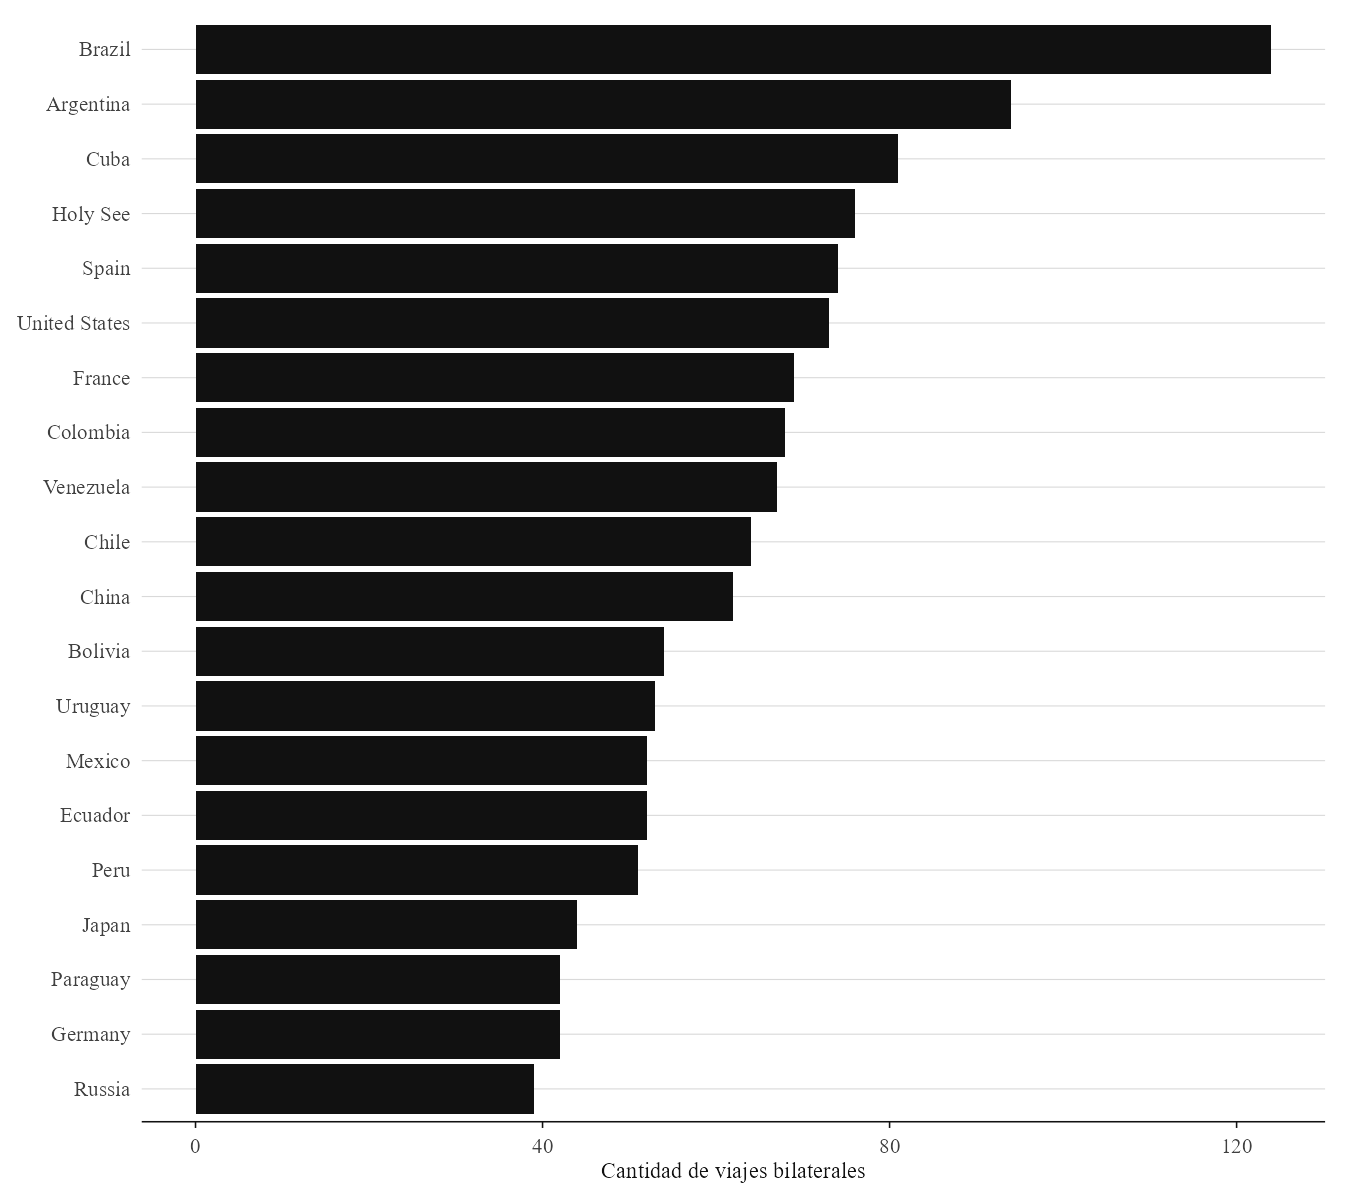
\includegraphics[width=0.85\textwidth]{../08_ANALISIS_R/outputs/09a_ranking_destinos_bilaterales.png}
  \caption{Los 20 destinos bilaterales m\'as visitados (viajes con reuni\'on registrada con el anfitri\'on).}
  \label{fig:ranking-bilateral}
\end{figure}

\begin{figure}[H]
  \centering
  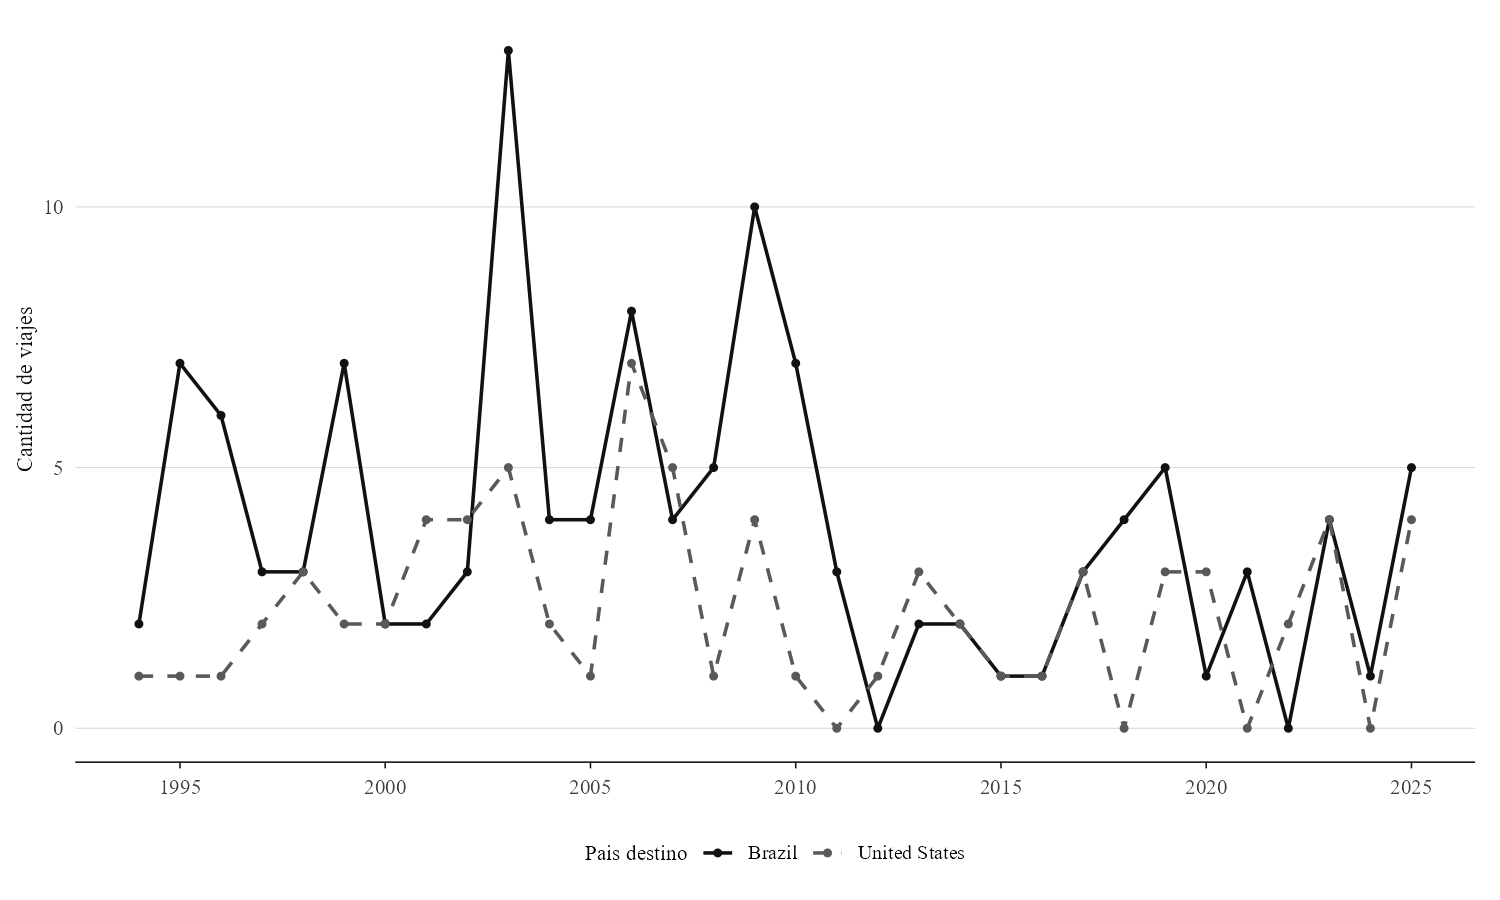
\includegraphics[width=0.85\textwidth]{../08_ANALISIS_R/outputs/09a2_evolucion_bilateral_brasil_eeuu.png}
  \caption{Evoluci\'on 1994-2025 de los viajes bilaterales a Brasil y Estados Unidos.}
  \label{fig:evolucion-bilateral-bra-arg-cuba}
\end{figure}

\begin{figure}[H]
  \centering
  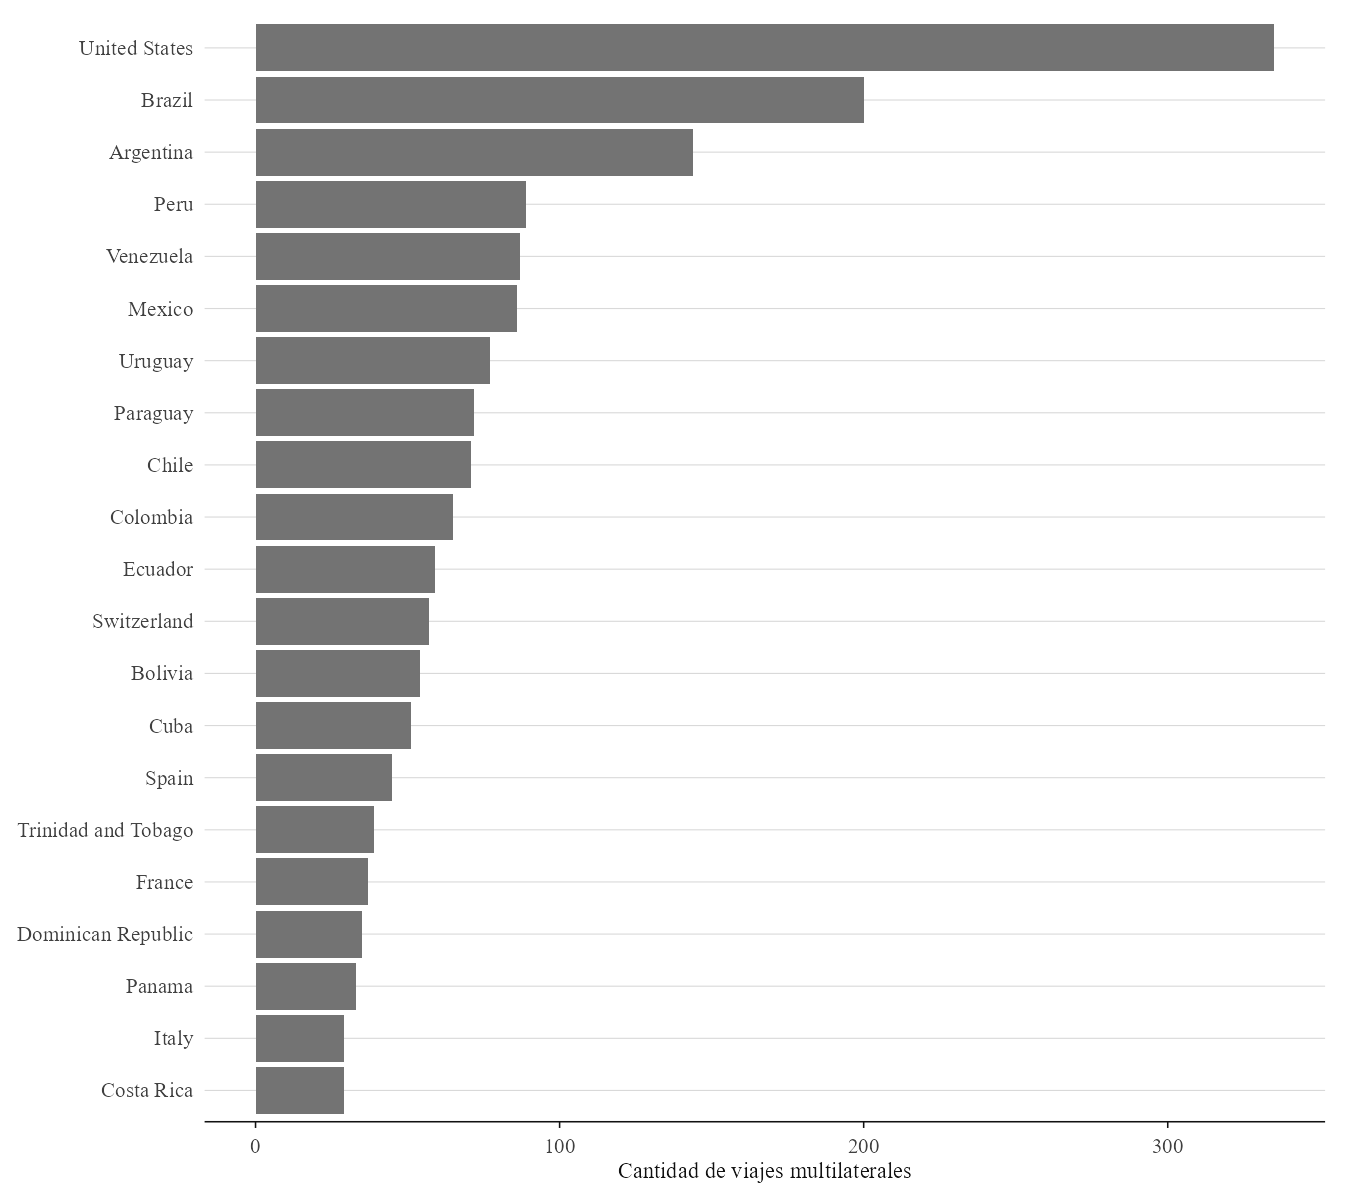
\includegraphics[width=0.85\textwidth]{../08_ANALISIS_R/outputs/09b_ranking_destinos_multilaterales.png}
  \caption{Los 20 destinos multilaterales m\'as visitados (viajes con asistencia a un evento multilateral).}
  \label{fig:ranking-multilateral}
\end{figure}

\begin{figure}[H]
  \centering
  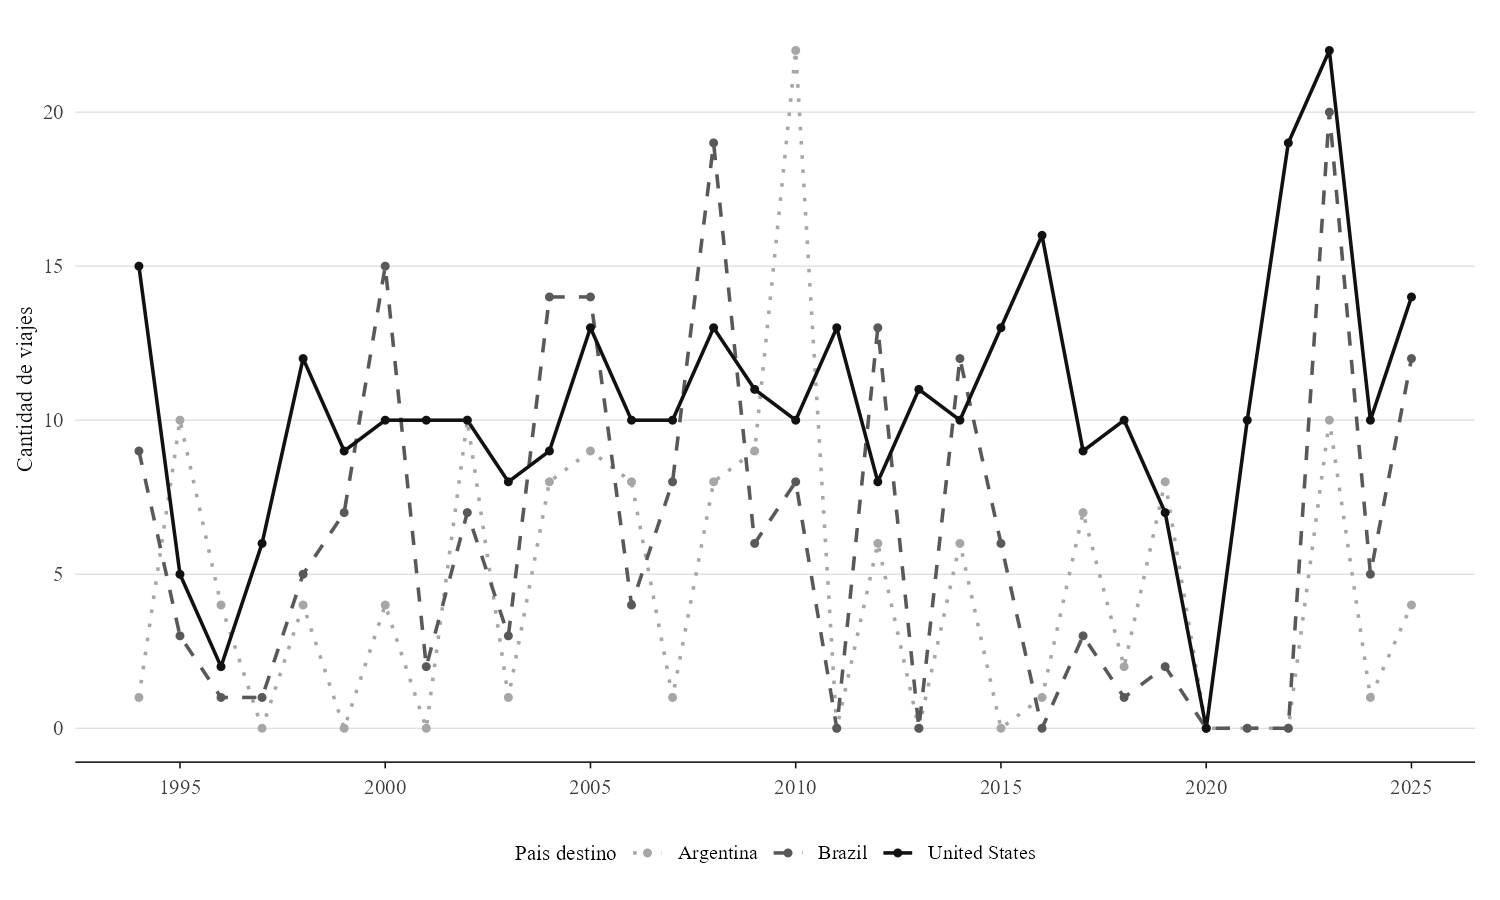
\includegraphics[width=0.85\textwidth]{../08_ANALISIS_R/outputs/09b2_evolucion_multilateral_usa_bra_arg.png}
  \caption{Evoluci\'on 1994-2025 de los viajes multilaterales a Estados Unidos, Brasil y Argentina.}
  \label{fig:evolucion-multilateral-usa-bra-arg}
\end{figure}

\begin{figure}[H]
  \centering
  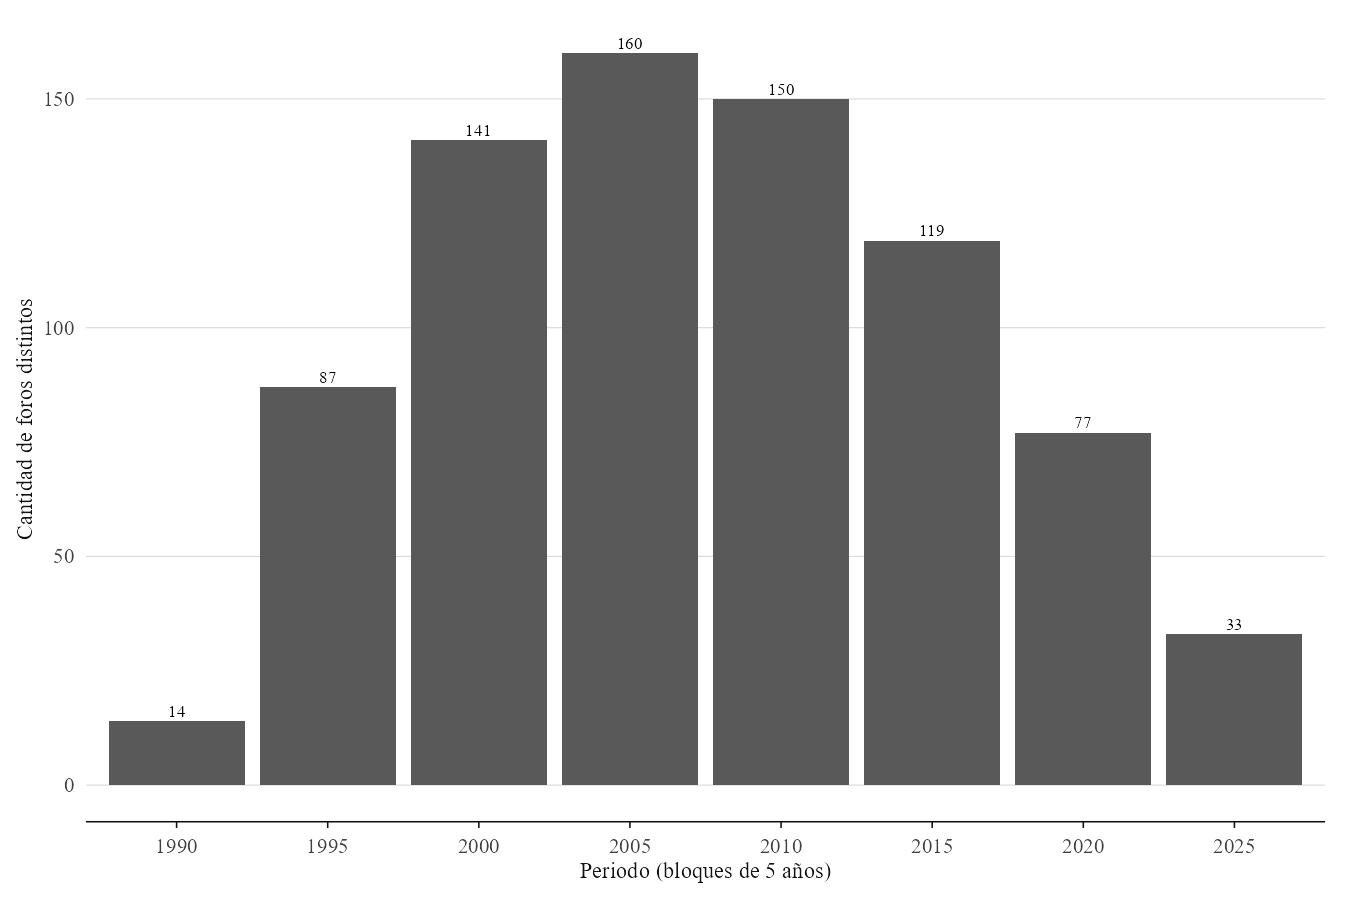
\includegraphics[width=0.85\textwidth]{../08_ANALISIS_R/outputs/09c_foros_distintos_por_periodo.png}
  \caption{Cantidad de foros/cumbres multilaterales distintos, por per\'iodo (idea: \citep{penaComplejaRedCumbres2005}).}
  \label{fig:foros-periodo}
\end{figure}

\begin{figure}[H]
  \centering
  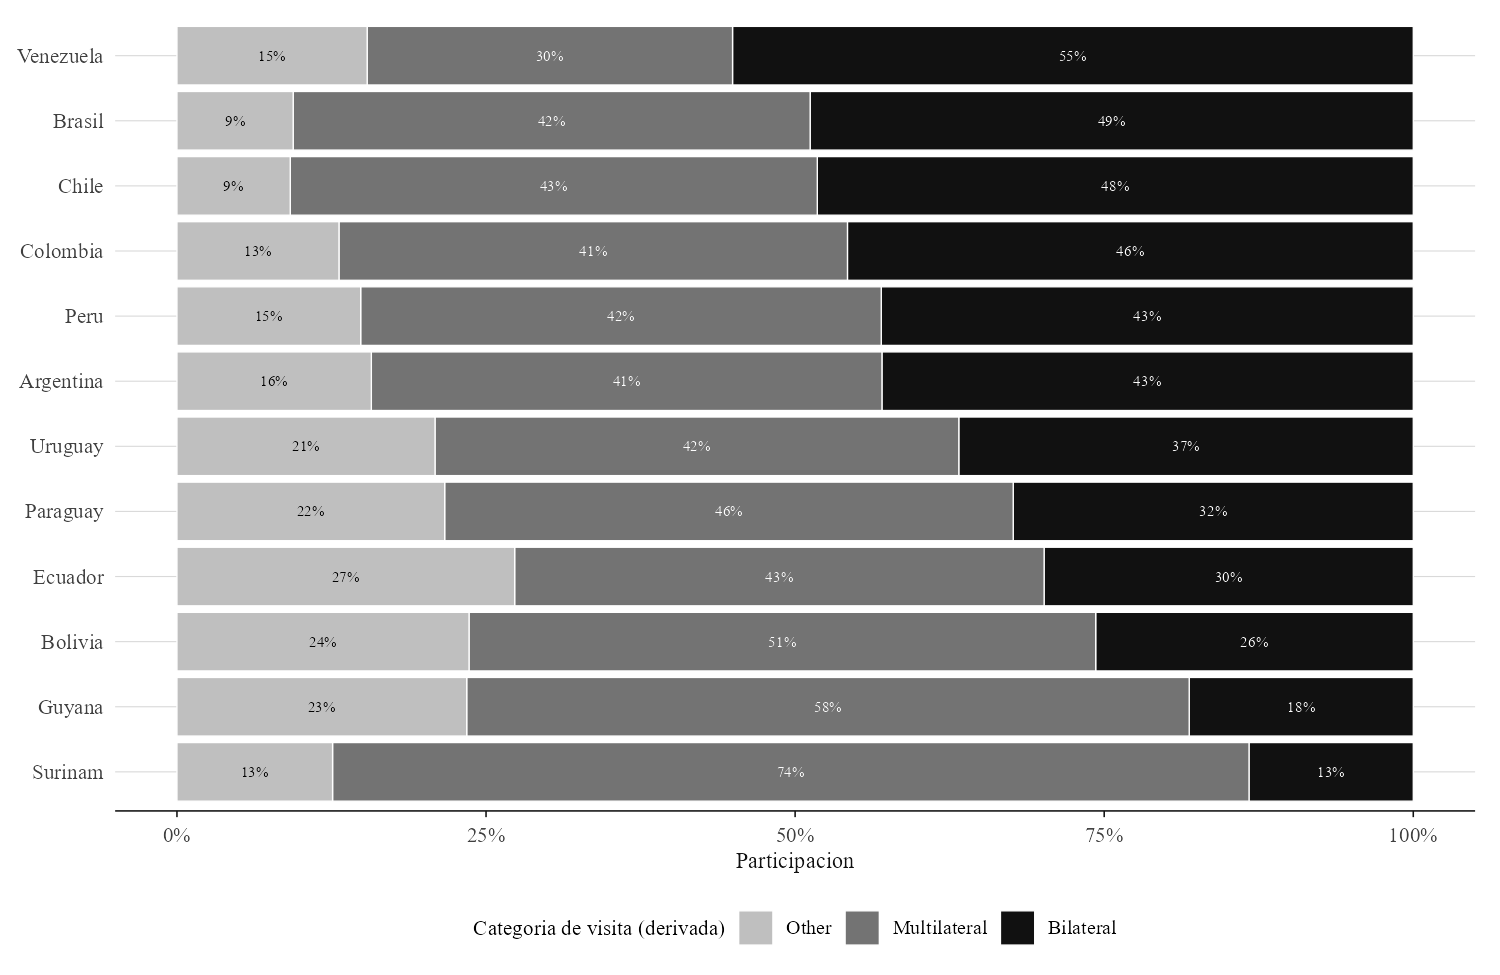
\includegraphics[width=0.9\textwidth]{../08_ANALISIS_R/outputs/09d_composicion_bilateral_multilateral_por_pais.png}
  \caption{Composici\'on Bilateral / Multilateral / Otro por pa\'is, con etiquetas de dato (an\'alisis composicional; m\'etodo: \citep{leeTravelAlliesAdversaries2024}). Se excluyen los viajes de categor\'ia ``Sin dato'' (ver Datos y metodolog\'ia) del c\'alculo.}
  \label{fig:composicion-pais}
\end{figure}

% Nota: 05_top5_destinos_por_presidente.csv y 06_primera_visita_por_presidente.csv
% son tablas completas (una fila por presidente) demasiado largas para el cuerpo
% del paper; queda a criterio de la redaccion si van como tabla resumida, anexo,
% o material suplementario. graficar_top_destinos("Nombre del mandatario") en
% graficos_exploratorios.R genera el detalle de un presidente puntual si hace
% falta un caso ilustrativo.

\subsection{Mandatarios, ideolog\'ia, cercan\'ia y comercio}
% Area 3 (pedido del usuario, pivot "Diplomacia Presidencial"): las 3
% dimensiones que el usuario pidio agrupar para explicar el comportamiento
% INDIVIDUAL de cada mandatario -por que viaja a donde viaja-: cercania
% geografica (el bloque de sesgo al vecino inmediato, movido aca desde la
% Situacion particular de los mandatarios), ideologia presidencial (sin
% cambios de contenido respecto de la version anterior, solo de numeracion
% de sub-seccion) y comercio (pendiente: falta que el usuario sume la base
% de datos de comercio bilateral correspondiente).

\subsubsection{Cercan\'ia geogr\'afica: el sesgo hacia el vecino inmediato}

% MOVIDO (2026-09-11) desde la ex-"Comparacion entre paises" (ahora
% "Situacion particular de los mandatarios"): el usuario pidio agrupar esta
% dimension junto con Ideologia y Comercio, como las 3 explicaciones del
% comportamiento individual de cada mandatario frente a los viajes. Sin
% cambios de contenido respecto de la version anterior.

\begin{figure}[H]
  \centering
  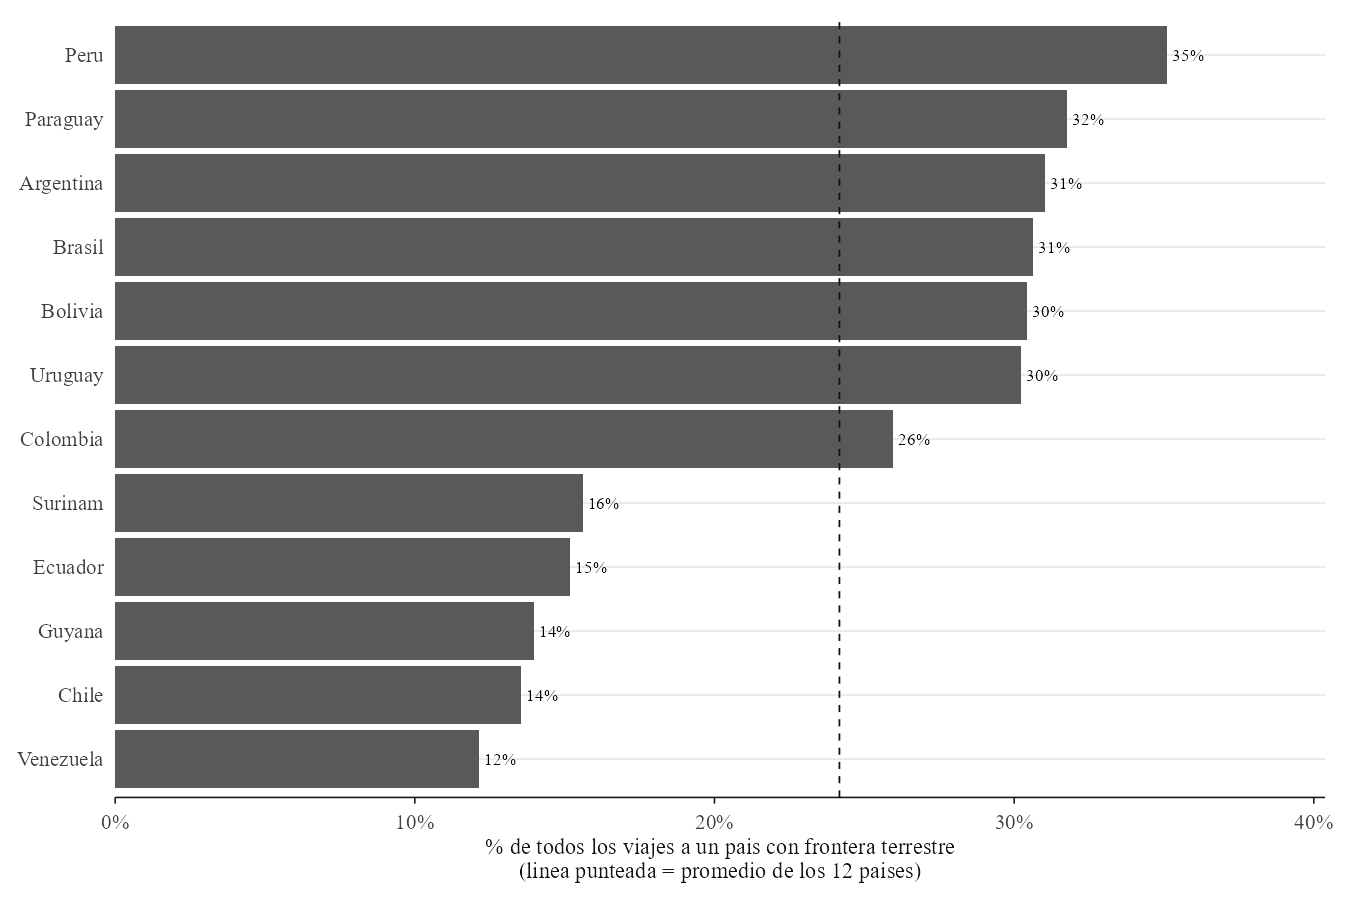
\includegraphics[width=0.85\textwidth]{../08_ANALISIS_R/outputs/14_sesgo_vecino_inmediato.png}
  % FIX (2026-09-10, item 2/pedido general "ningun grafico cortado"):
  % \colorbox{yellow}{...} envolviendo TODO el caption es una caja no
  % quebrable -provocaba un Overfull hbox de 1334pt-. \parbox adentro del
  % colorbox permite que el texto quiebre en varias lineas y se mantiene el
  % resaltado amarillo (el usuario confirmo mantenerlo).
  \caption{\colorbox{yellow}{\parbox{\dimexpr\textwidth-2\fboxsep\relax}{Porcentaje de TODOS los viajes (no s\'olo el primero) que van a un pa\'is con frontera terrestre, por pa\'is de origen. Ostrander \& Rider (2018) encuentran que 7 de 10 presidentes de EE.\,UU. eligen un vecino como primer destino; ac\'a se prueba si el patr\'on se sostiene para el conjunto completo de viajes en Sudam\'erica (ver \citep{ostranderPresidentsAbroadPolitics2018}).}}}
  \label{fig:sesgo-vecino-inmediato}
\end{figure}
% NOTA: descripcion resaltada en amarillo a pedido del usuario -no esta
% seguro de dejar esta figura en el paper; revisar antes de la version final.

% Cuadro Nuevo (pedido del usuario, despues de la Figura 18): correlacion
% entre viaje presidencial y visitar un vecino fronterizo vs. otro pais, A
% LO LARGO DE TODA LA SERIE (la Figura anterior da un solo valor agregado
% 1994-2025; esta ve la evolucion anio a anio). Se apoya en una base nueva
% de referencia -diadas Origen (12 paises de la base de viajes) x Destino
% (paises efectivamente visitados), con una columna Es_Vecino_Fronterizo y
% los codigos ISO alpha-3 de LeaderCountryISO/CountryVisitedISO- guardada en
% 04\_BASE\_FINAL/Base\_Diadas\_Vecinos.xlsx.

% latex table generated in R 4.5.1 by xtable 1.8-8 package
% Fri Sep 11 10:51:23 2026
\begin{table}[ht]
\centering
\caption{Correlaci\'on de Pearson entre el a\~no (tiempo) y el \% de viajes a un vecino fronterizo, 1994-2025 (una observaci\'on por a\~no).} 
\label{tab:correlacion-vecino}
\begin{tabular}{lrrr}
  \hline
Variable & r & p.valor & n\_anios \\ 
  \hline
Anio (tiempo) vs. \% de viajes a un vecino fronterizo & -0.43 & 0.01 &  32 \\ 
   \hline
\end{tabular}
\end{table}
\begin{figure}[H]
  \centering
  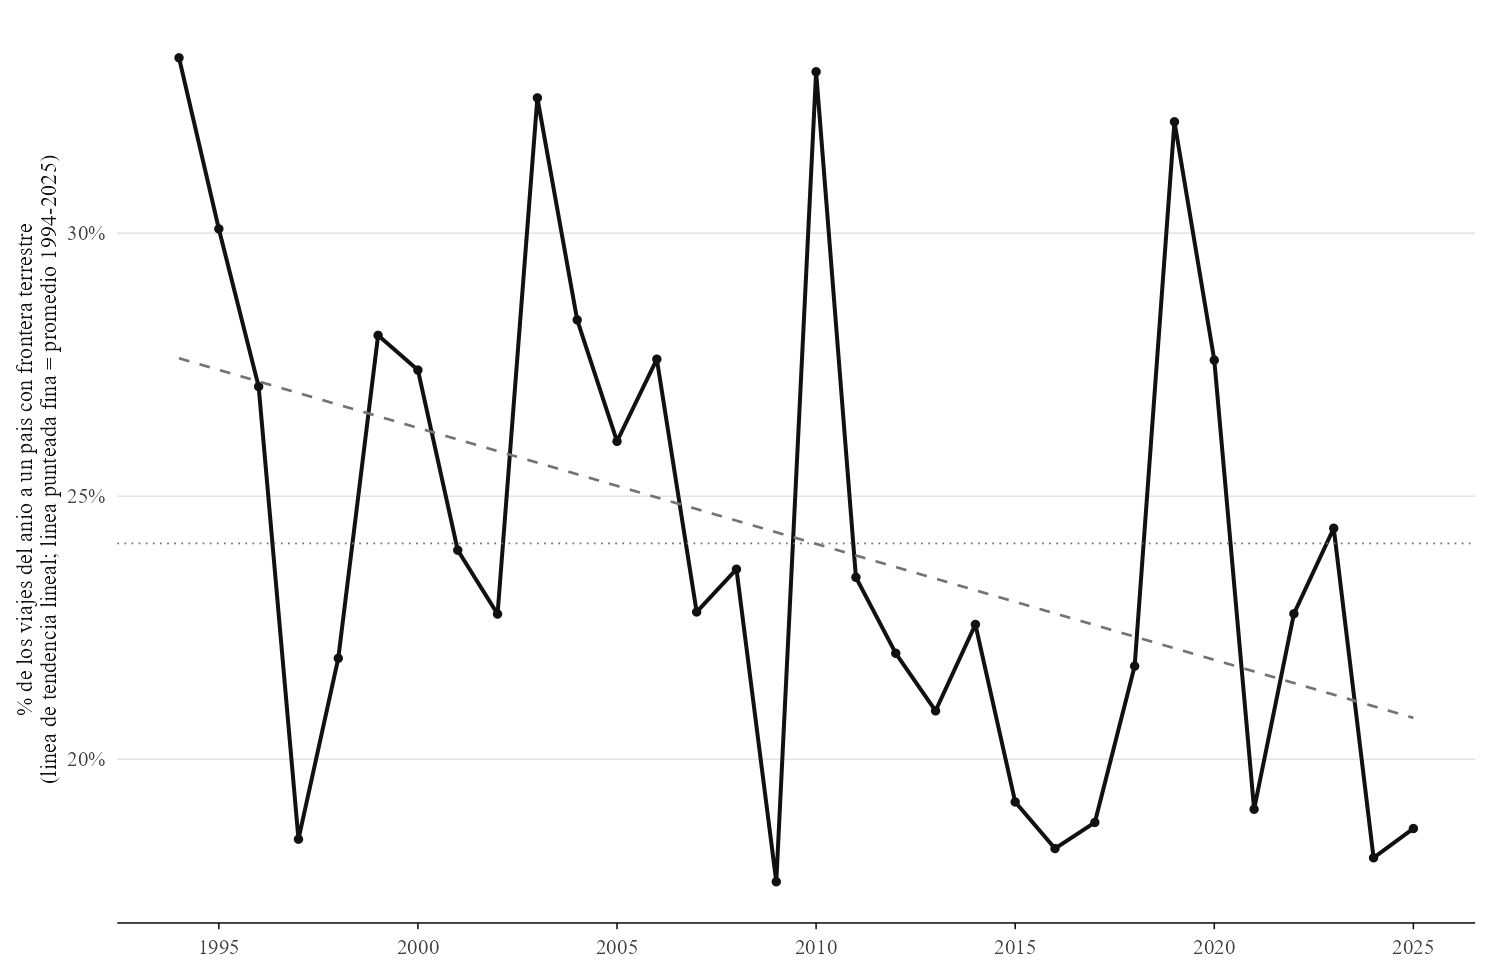
\includegraphics[width=0.85\textwidth]{../08_ANALISIS_R/outputs/14b_vecino_fronterizo_a_lo_largo_del_tiempo.png}
  \caption{Porcentaje de los viajes de cada a\~no dirigidos a un pa\'is con frontera terrestre (los 12 pa\'ises de la base en conjunto), 1994-2025, con l\'inea de tendencia lineal. Extiende la Figura~\ref{fig:sesgo-vecino-inmediato} -que da un solo valor agregado para todo el per\'iodo- a una serie temporal, para ver si el sesgo hacia el vecino inmediato crece, se mantiene o cae con el correr del tiempo.}
  \label{fig:vecino-a-lo-largo-del-tiempo}
\end{figure}

\subsubsection{Viajes e ideolog\'ia presidencial}

% Fuente de ideologia: base propia (04_BASE_FINAL/Base_Ideologia_Presidencial.xlsx),
% que combina \citep{merkeForeignPolicyChange2020} (Merke, Reynoso \& Schenoni 2020,
% 140 mandatos-termino, encuesta a expertos 1-7 en 8 dimensiones) con una
% actualizacion propia ("CPE - Latinoamerica") que extiende la cobertura a 23
% mandatos-termino mas recientes (hasta ~2020) con la misma metodologia. El
% cruce contra los viajes usa un crosswalk propio de Leader_key + fecha exacta
% de asuncion/reeleccion (no el "yearinoffice" de la base de ideologia, que en
% varios casos no coincide con la fecha real de asuncion; ver
% 08_ANALISIS_R/graficos_exploratorios.R, seccion 18, para el detalle completo
% de cada fecha usada). Jeanine A\~nez (Bolivia) y Francisco Sagasti (Peru)
% quedan fuera de este cruce -estan en la base de ideologia pero no tienen
% viajes cargados ni fecha de mandato verificada en nuestra base; ver
% 05_BITACORA/PENDIENTES\_VERIFICACION.txt-.

Esta secci\'on examina si la orientaci\'on ideol\'ogica de cada presidente se asocia con la proporci\'on de sus viajes dirigidos a Am\'erica Latina. Se utilizan las ocho dimensiones relevadas por la encuesta a expertos de \citep{merkeForeignPolicyChange2020} (ideolog\'ia general, pol\'itica econ\'omica, geopol\'itica, estilo diplom\'atico, relaci\'on con Estados Unidos, soberan\'ia/autonom\'ia, modelo de desarrollo y reputaci\'on internacional), cada una en una escala de 1 a 7. La unidad de observaci\'on es el mandato-tramo (un presidente reelegido aporta una observaci\'on por cada per\'iodo, ya que su valor de ideolog\'ia puede cambiar de un mandato a otro); se exigi\'o un m\'inimo de 5 viajes por tramo para evitar que porcentajes calculados sobre muestras muy chicas distorsionen la comparaci\'on. Toda la secci\'on se restringe a viajes de categor\'ia \textbf{Bilateral} (se excluyen Multilateral, Other y Sin dato): un viaje a una cumbre multilateral no refleja una preferencia bilateral real del presidente por ese destino seg\'un su propia ideolog\'ia, sino la ubicaci\'on del foro (mismo criterio ya aplicado en el Cuadro~\ref{tab:destino-favorito} de destino favorito). La secci\'on se divide en dos partes: la parte A) mide estas dimensiones contra el \textbf{porcentaje} de viajes intra-latinoamericanos de cada mandato-tramo; la parte B) repite exactamente los mismos cruces pero contra la \textbf{cantidad absoluta} de viajes intra-latinoamericanos, para chequear si el patr\'on de la parte A) se sostiene al mirar el volumen bruto de viajes en vez de la proporci\'on -un mandato-tramo con pocos viajes en total puede tener un \% alto de viajes intralatam pero un n\'umero absoluto chico, y viceversa-.

\subsubsection*{A) Ideolog\'ia presidencial y \% de viajes intralatinoamericanos}

% latex table generated in R 4.5.1 by xtable 1.8-8 package
% Fri Sep 11 10:51:23 2026
\begin{table}[ht]
\centering
\caption{Correlaci\'on de Pearson entre cada dimensi\'on de ideolog\'ia presidencial y el \% de viajes intra-latinoamericanos, por mandato-tramo (1994-2025, solo viajes Bilaterales).} 
\label{tab:correlacion-ideologia}
\begin{tabular}{lrrr}
  \hline
Dimension & r\_pearson & valor\_p & n\_mandatos \\ 
  \hline
Ideologia general (1=izq., 7=der.) & -0.06 & 0.63 &  66 \\ 
  Politica economica & -0.05 & 0.70 &  66 \\ 
  Geopolitica & -0.02 & 0.89 &  66 \\ 
  Estilo diplomatico & 0.02 & 0.85 &  66 \\ 
  Relacion con EE.UU. & -0.05 & 0.71 &  66 \\ 
  Soberania / autonomia & 0.06 & 0.64 &  66 \\ 
  Modelo de desarrollo & -0.08 & 0.51 &  66 \\ 
  Reputacion internacional & -0.06 & 0.64 &  66 \\ 
   \hline
\end{tabular}
\end{table}
\begin{figure}[H]
  \centering
  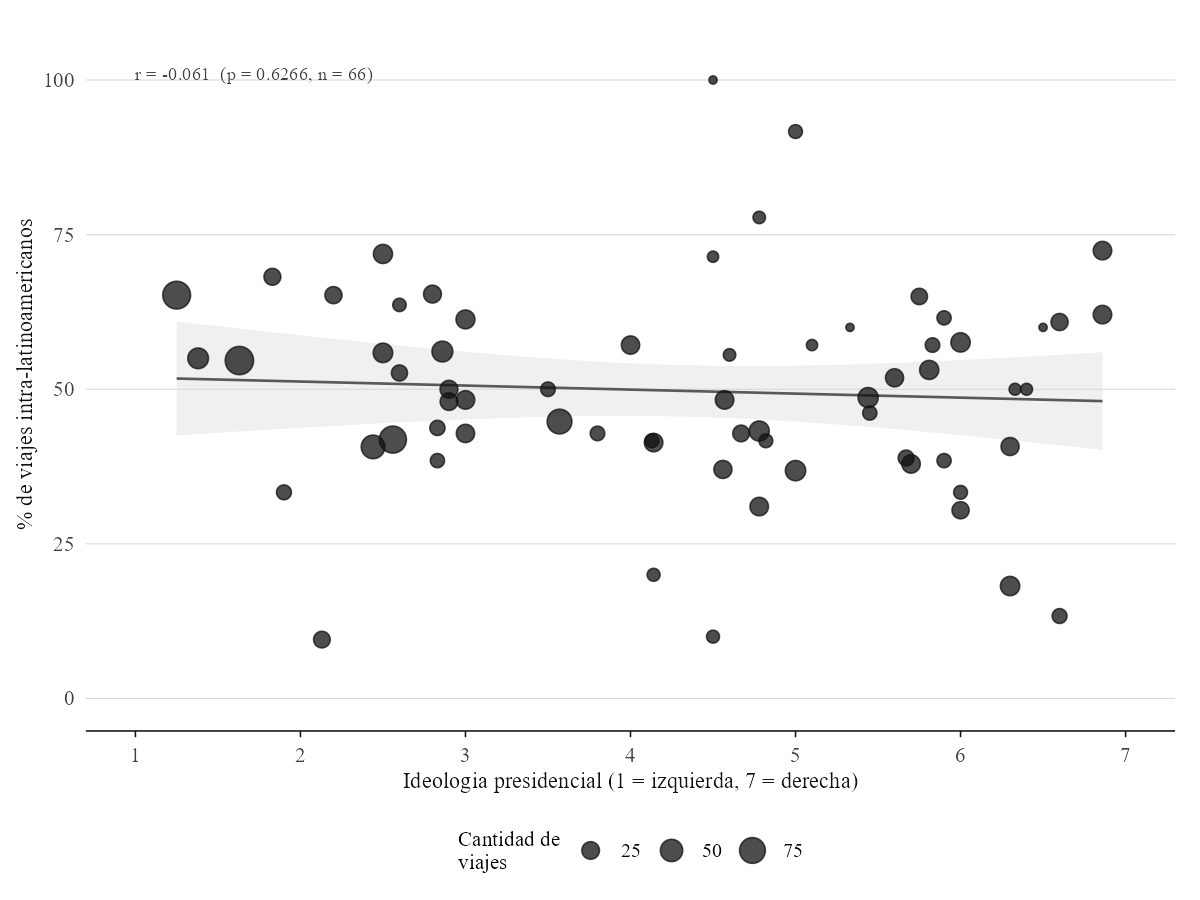
\includegraphics[width=0.85\textwidth]{../08_ANALISIS_R/outputs/18c_ideologia_vs_intralatam.png}
  \caption{Ideolog\'ia presidencial general (1 = izquierda, 7 = derecha) vs. \% de viajes intra-latinoamericanos, un punto por mandato-tramo. Este es el hallazgo central de \citep{merkeForeignPolicyChange2020} -la ideolog\'ia presidencial es la variable que m\'as explica el cambio de pol\'itica exterior- puesto a prueba espec\'ificamente para el enfoque regional de los viajes.}
  \label{fig:ideologia-vs-intralatam}
\end{figure}

\begin{figure}[H]
  \centering
  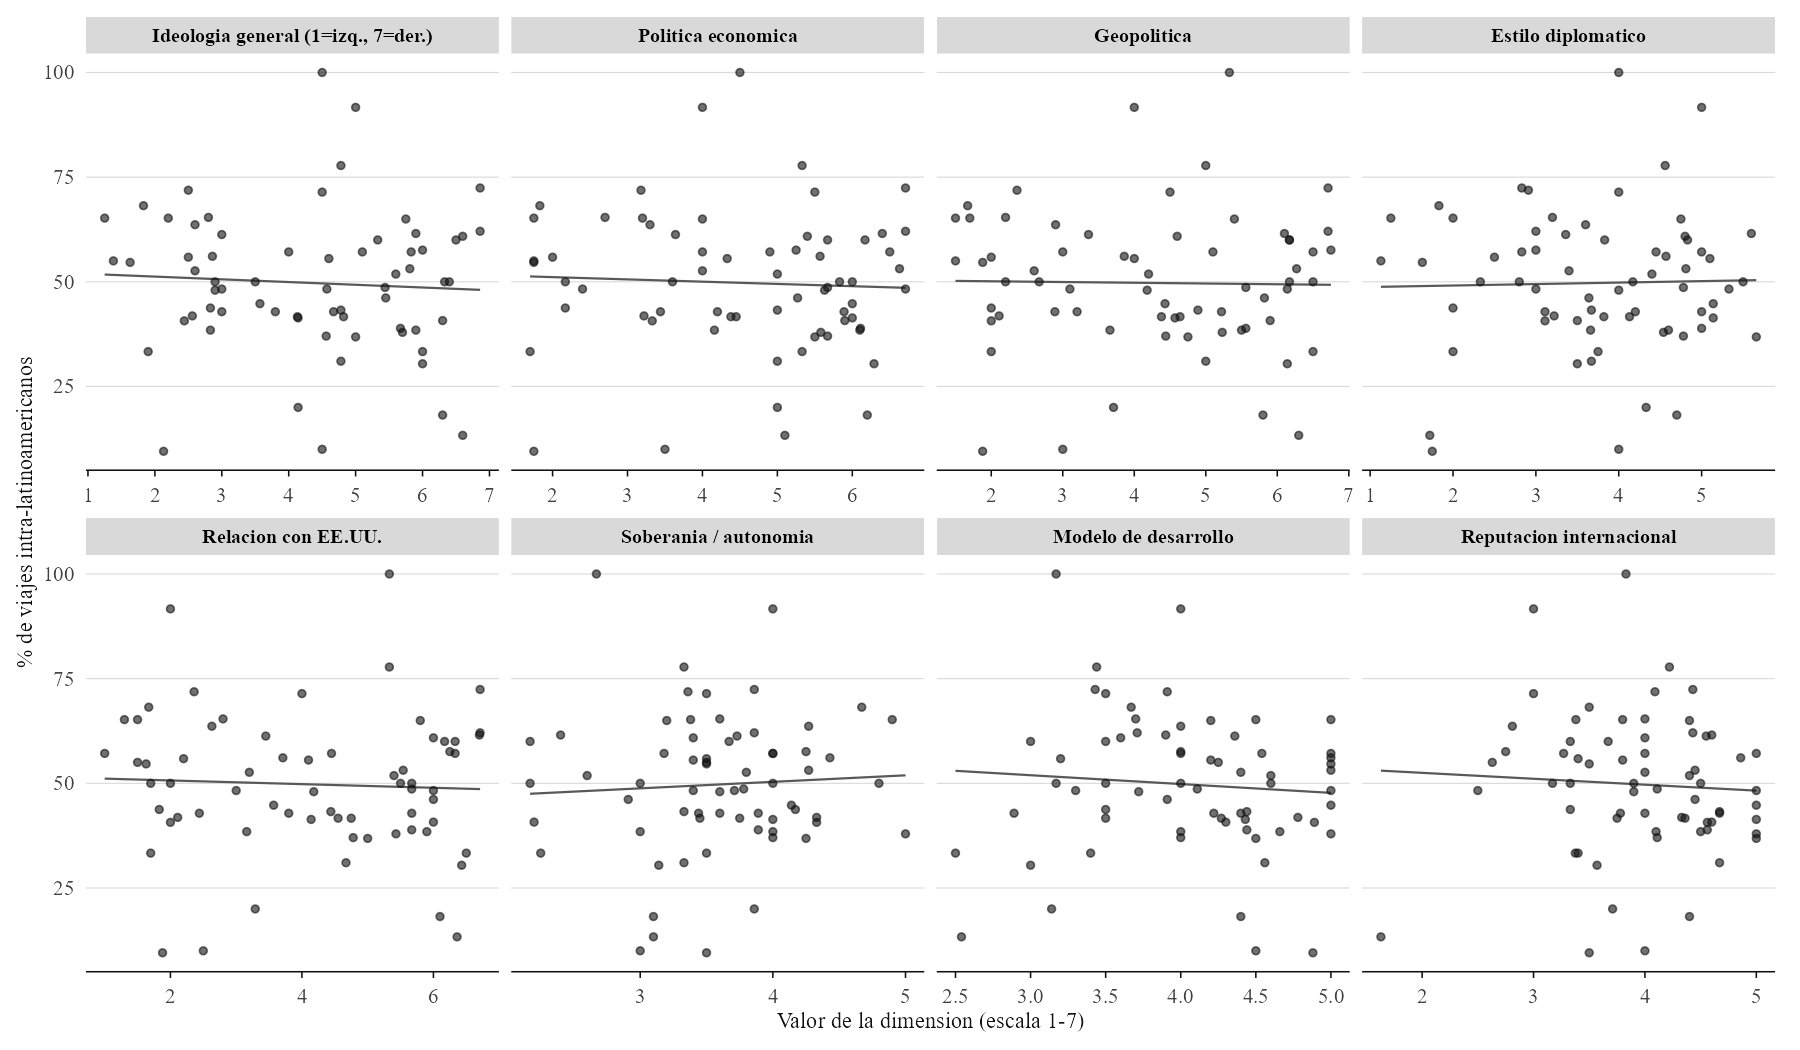
\includegraphics[width=\textwidth]{../08_ANALISIS_R/outputs/18d_todas_dimensiones_vs_intralatam.png}
  \caption{Las ocho dimensiones de ideolog\'ia presidencial vs. \% de viajes intra-latinoamericanos.}
  \label{fig:todas-dimensiones-intralatam}
\end{figure}

% 3 variantes de la figura anterior (pedido del usuario): mandato-tramos de
% ideologia general baja (izquierda) y alta (derecha) por separado, y
% restringido a los ultimos 10 anios con dato disponible (2012-2022).
\begin{figure}[H]
  \centering
  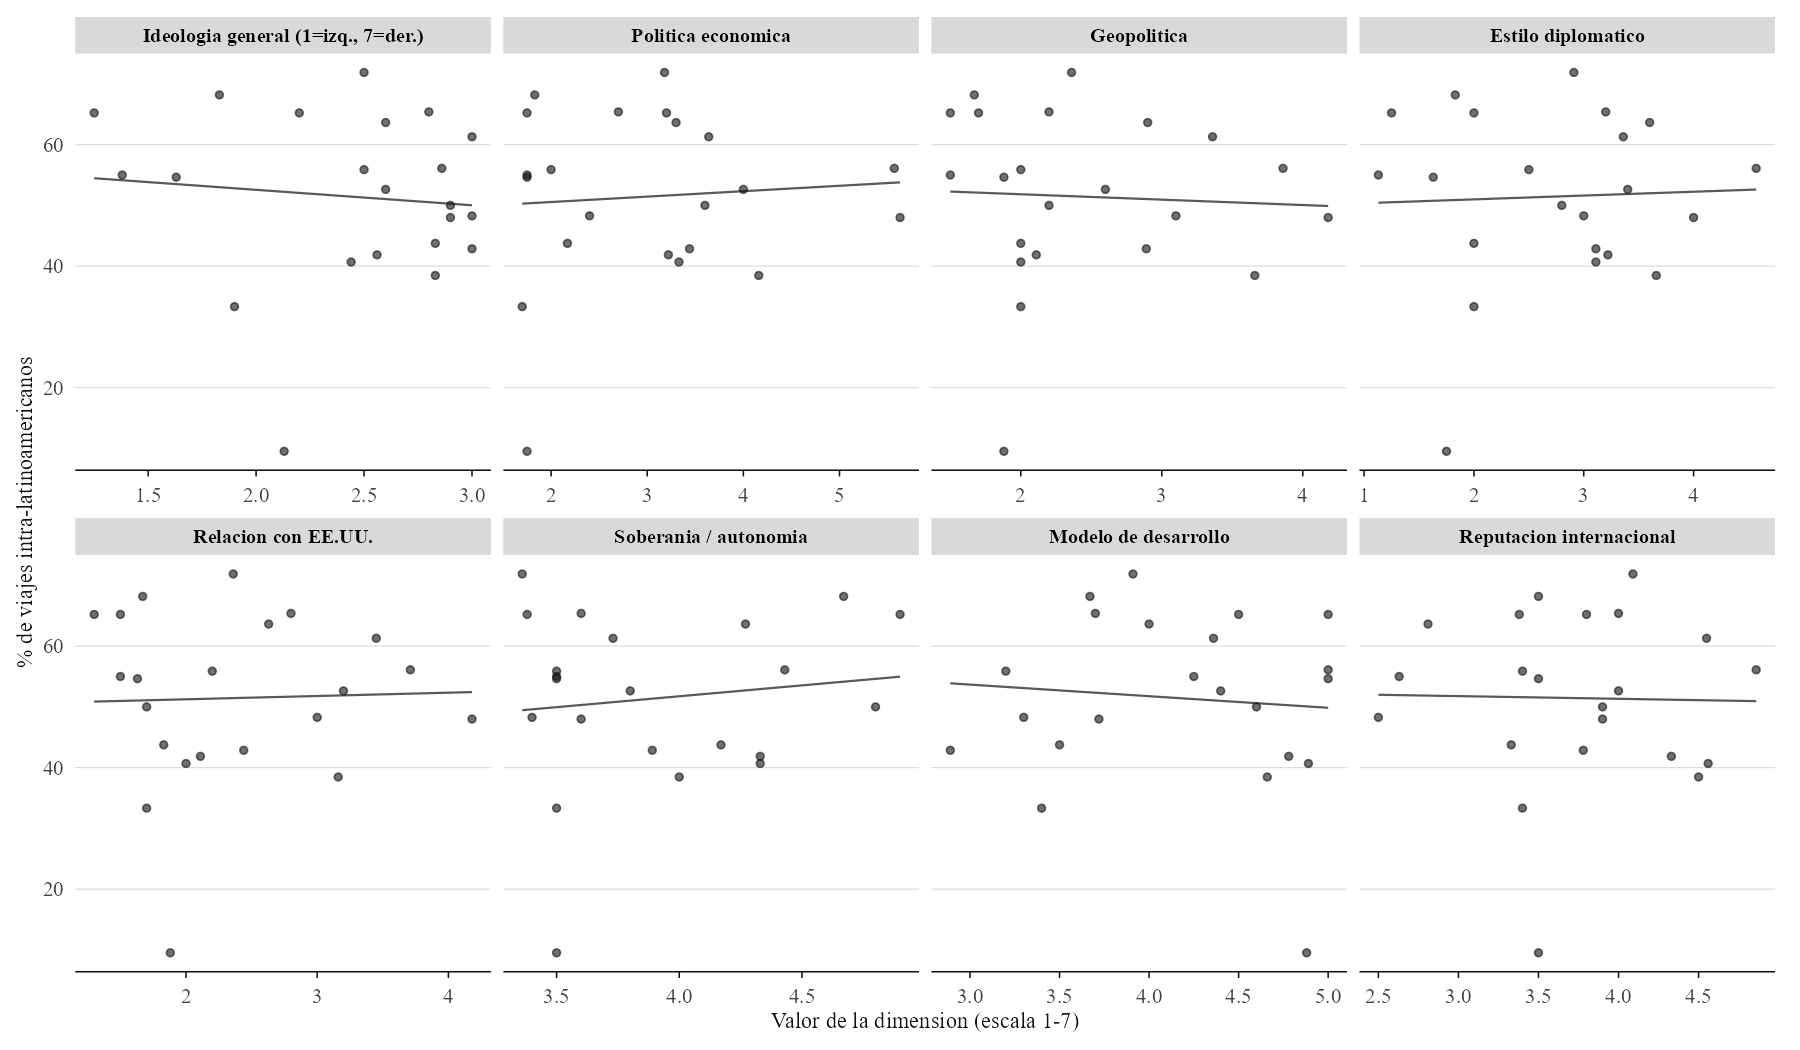
\includegraphics[width=\textwidth]{../08_ANALISIS_R/outputs/18i_todas_dimensiones_izquierda.png}
  \caption{Las ocho dimensiones de ideolog\'ia presidencial vs. \% de viajes intra-latinoamericanos, restringido a mandato-tramos de ideolog\'ia general BAJA (izquierda, $\leq 3$ en la escala 1-7). Compara con la Figura~\ref{fig:todas-dimensiones-derecha} para ver si el patr\'on difiere seg\'un el bloque ideol\'ogico.}
  \label{fig:todas-dimensiones-izquierda}
\end{figure}

\begin{figure}[H]
  \centering
  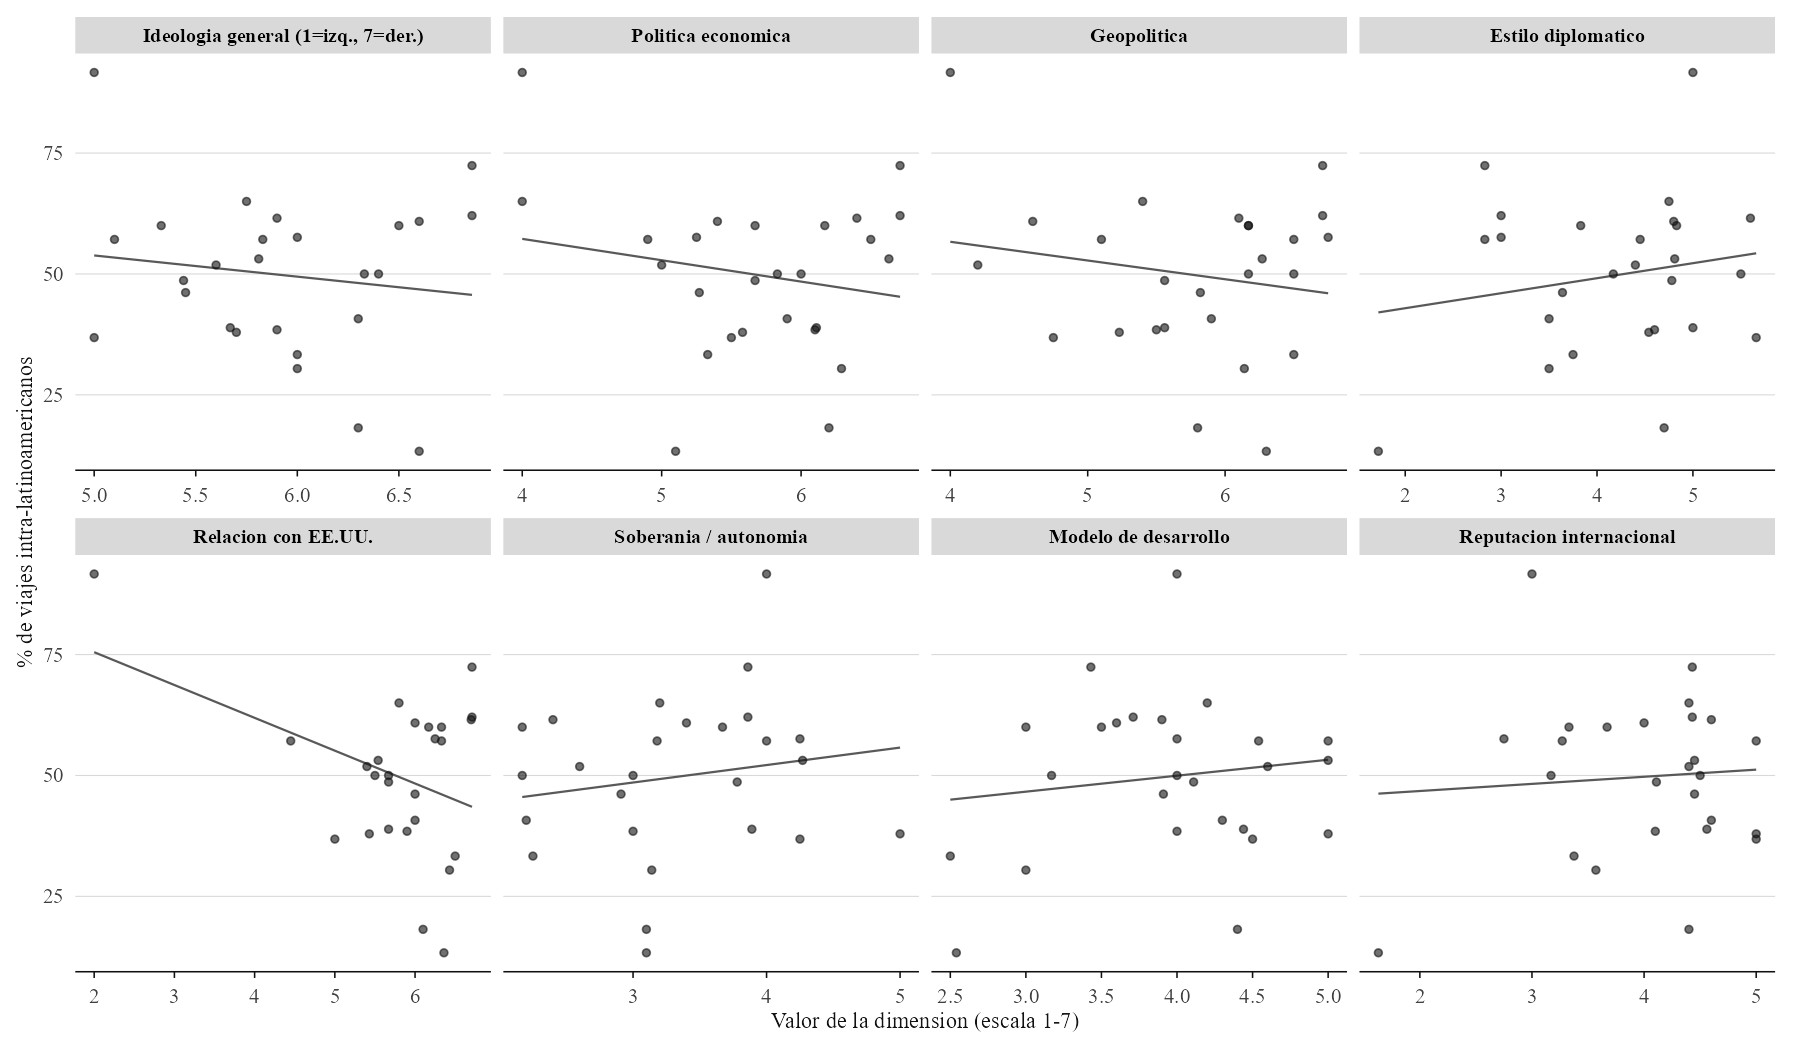
\includegraphics[width=\textwidth]{../08_ANALISIS_R/outputs/18j_todas_dimensiones_derecha.png}
  \caption{Las ocho dimensiones de ideolog\'ia presidencial vs. \% de viajes intra-latinoamericanos, restringido a mandato-tramos de ideolog\'ia general ALTA (derecha, $\geq 5$ en la escala 1-7).}
  \label{fig:todas-dimensiones-derecha}
\end{figure}

\begin{figure}[H]
  \centering
  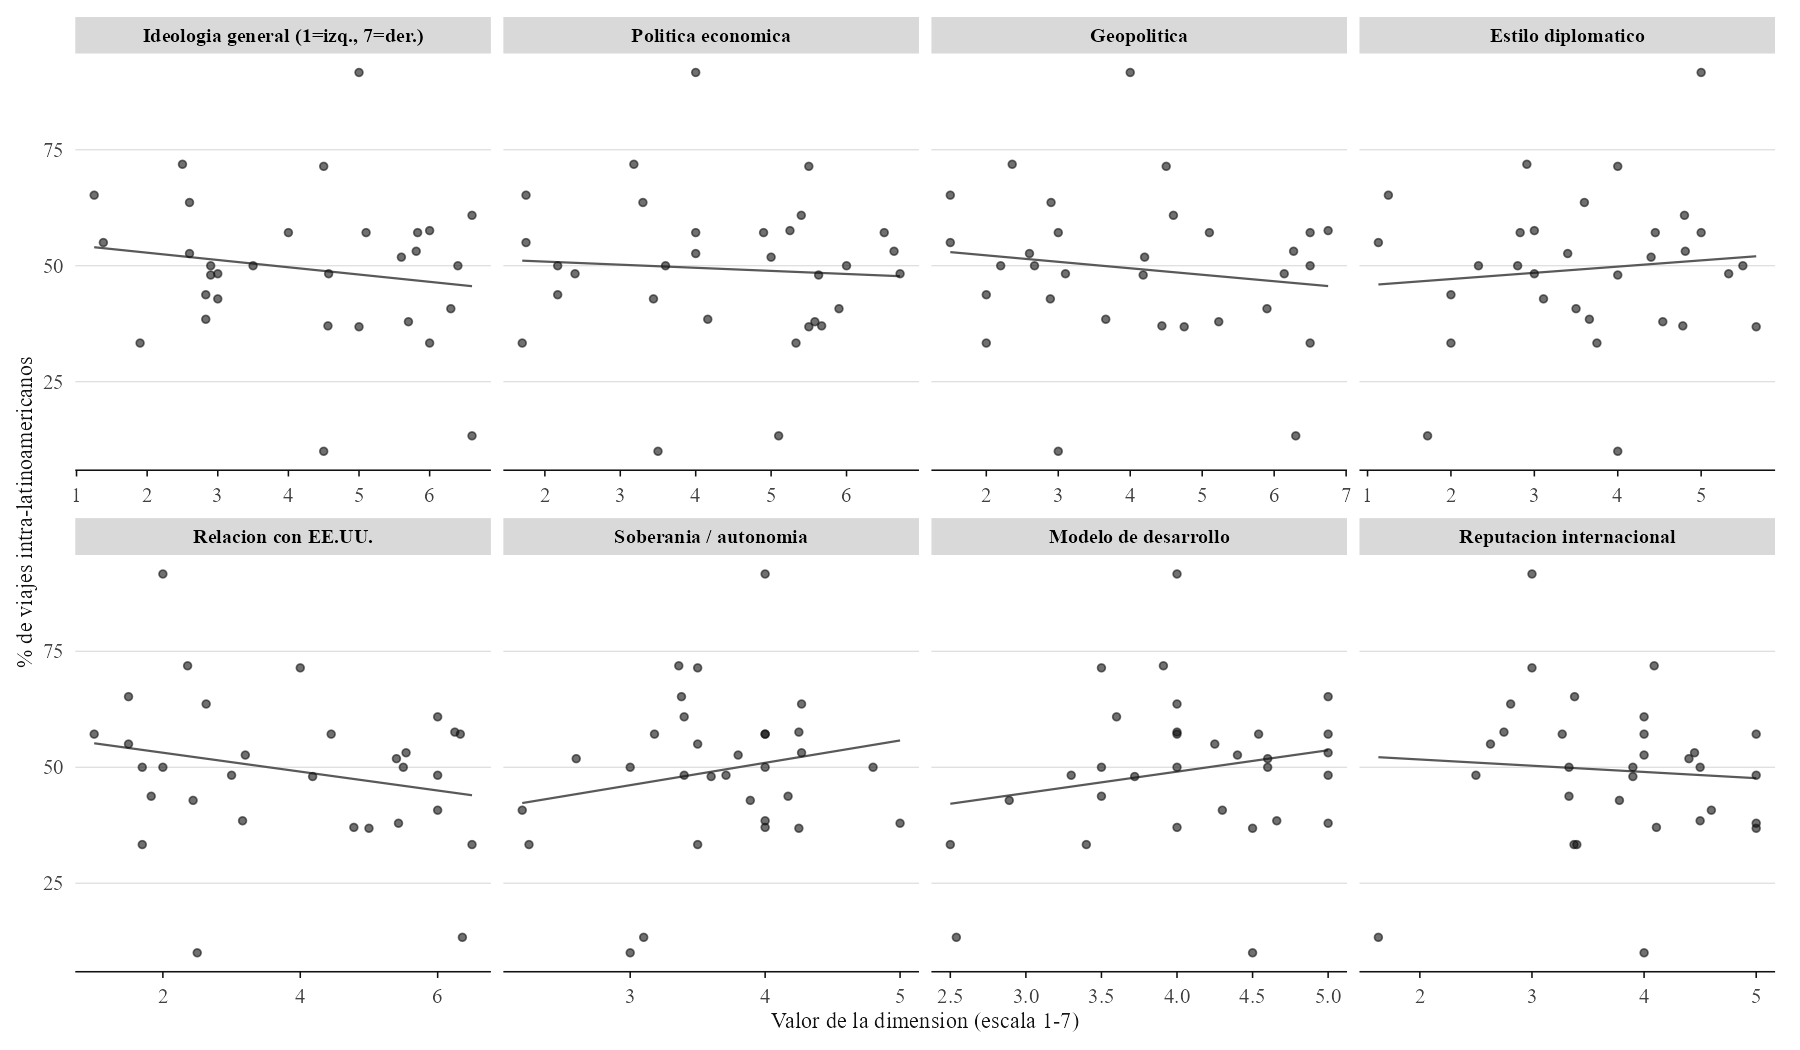
\includegraphics[width=\textwidth]{../08_ANALISIS_R/outputs/18k_todas_dimensiones_2012_2022.png}
  \caption{Las ocho dimensiones de ideolog\'ia presidencial vs. \% de viajes intra-latinoamericanos, restringido a mandato-tramos que se solapan con la ventana 2012-2022 (los \'ultimos 10 a\~nos con dato de ideolog\'ia disponible).}
  \label{fig:todas-dimensiones-2012-2022}
\end{figure}

\subsubsection*{B) Ideolog\'ia presidencial y cantidad ABSOLUTA de viajes latinoamericanos}

% Cuadro NUEVO (2026-09-06, pedido del usuario): mismo cruce que el Cuadro
% de la parte A), pero contra la CANTIDAD ABSOLUTA de viajes intra-latinoamericanos
% en vez del porcentaje.
% latex table generated in R 4.5.1 by xtable 1.8-8 package
% Fri Sep 11 10:51:23 2026
\begin{table}[ht]
\centering
\caption{Correlaci\'on de Pearson entre cada dimensi\'on de ideolog\'ia presidencial y la cantidad ABSOLUTA de viajes intra-latinoamericanos, por mandato-tramo (1994-2025, solo viajes Bilaterales).} 
\label{tab:correlacion-ideologia-absoluto}
\begin{tabular}{lrrr}
  \hline
Dimension & r\_pearson & valor\_p & n\_mandatos \\ 
  \hline
Ideologia general (1=izq., 7=der.) & -0.44 & 0.00 &  66 \\ 
  Politica economica & -0.32 & 0.01 &  66 \\ 
  Geopolitica & -0.38 & 0.00 &  66 \\ 
  Estilo diplomatico & -0.34 & 0.01 &  66 \\ 
  Relacion con EE.UU. & -0.36 & 0.00 &  66 \\ 
  Soberania / autonomia & 0.26 & 0.03 &  66 \\ 
  Modelo de desarrollo & 0.42 & 0.00 &  66 \\ 
  Reputacion internacional & 0.08 & 0.50 &  66 \\ 
   \hline
\end{tabular}
\end{table}
% Figura NUEVA (2026-09-06, pedido del usuario): misma figura de la parte A),
% pero contra la CANTIDAD ABSOLUTA de viajes intra-latinoamericanos en vez del \%.
\begin{figure}[H]
  \centering
  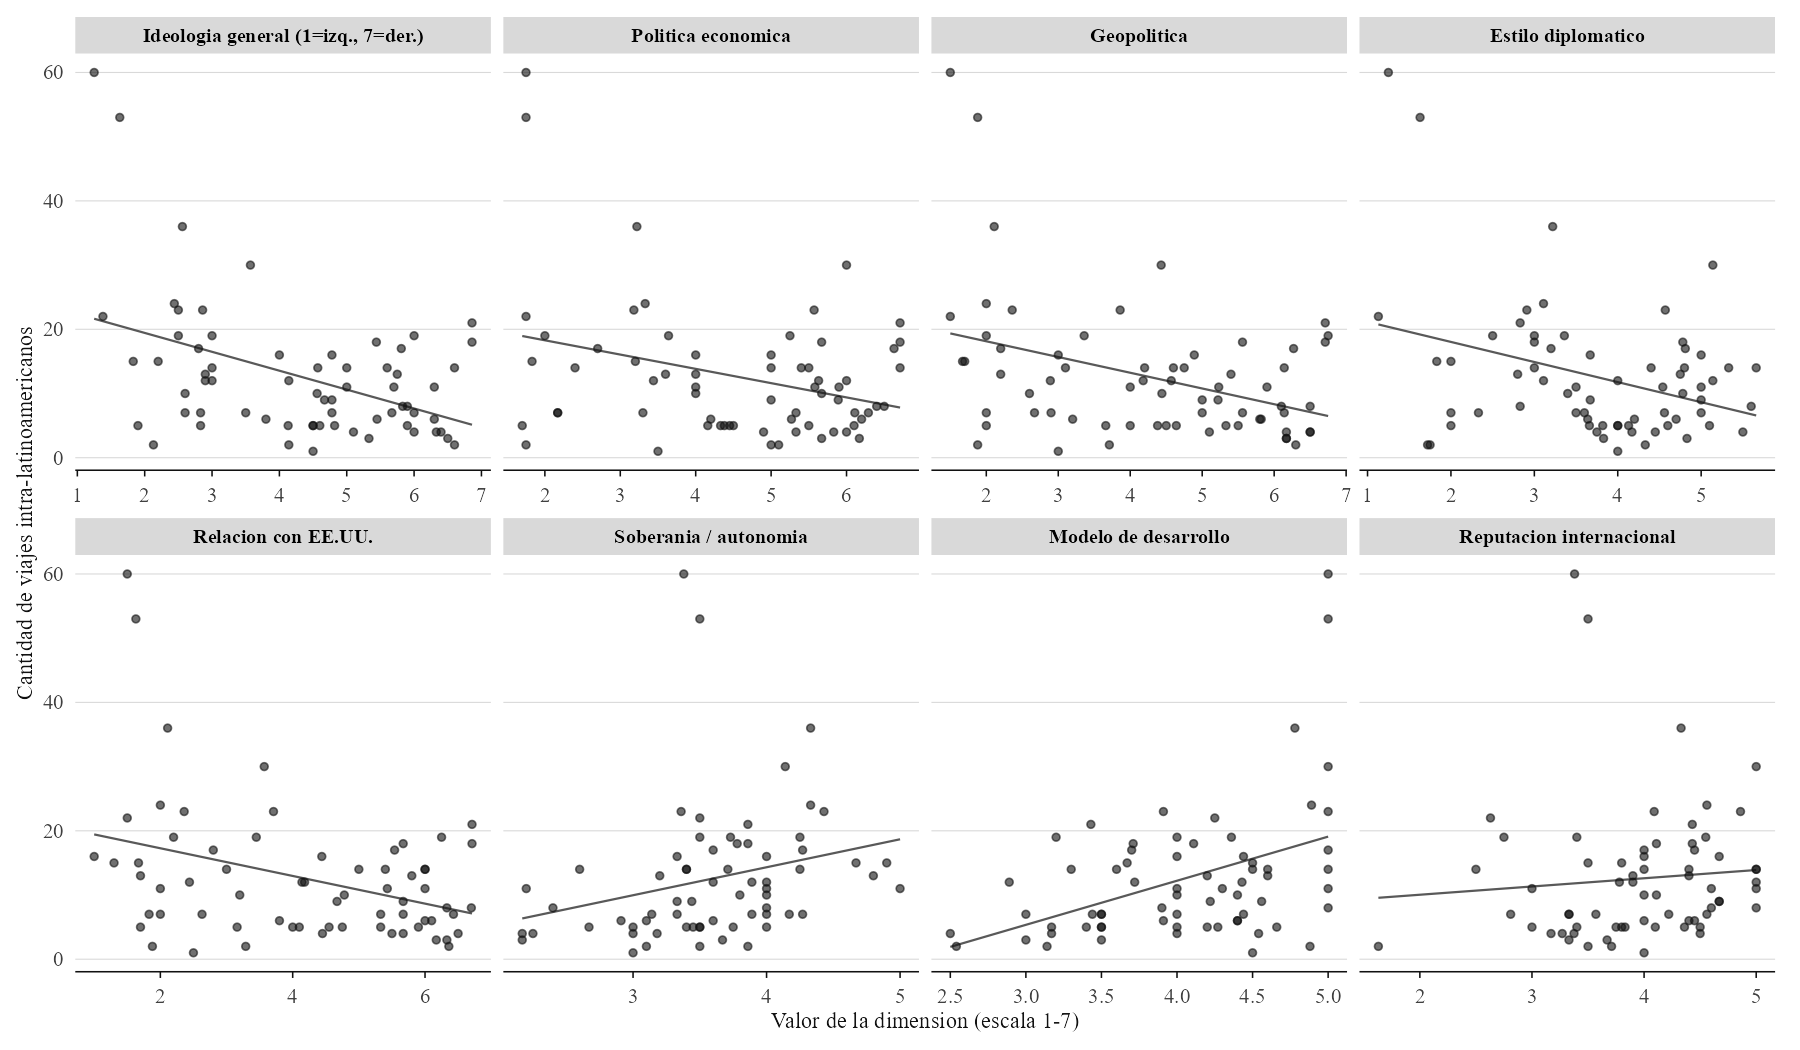
\includegraphics[width=\textwidth]{../08_ANALISIS_R/outputs/18d2_todas_dimensiones_vs_intralatam_absoluto.png}
  \caption{Las ocho dimensiones de ideolog\'ia presidencial vs. cantidad ABSOLUTA de viajes intra-latinoamericanos (compara con la Figura~\ref{fig:todas-dimensiones-intralatam}, que usa el \% en vez del valor absoluto).}
  \label{fig:todas-dimensiones-intralatam-absoluto}
\end{figure}

% 3 figuras NUEVAS (2026-09-10, pedido del usuario, item 13): contraparte
% ABSOLUTA de las 3 variantes izquierda/derecha/2012-2022 de la parte A),
% para que la parte B) quede completa y paralela a la parte A).
\begin{figure}[H]
  \centering
  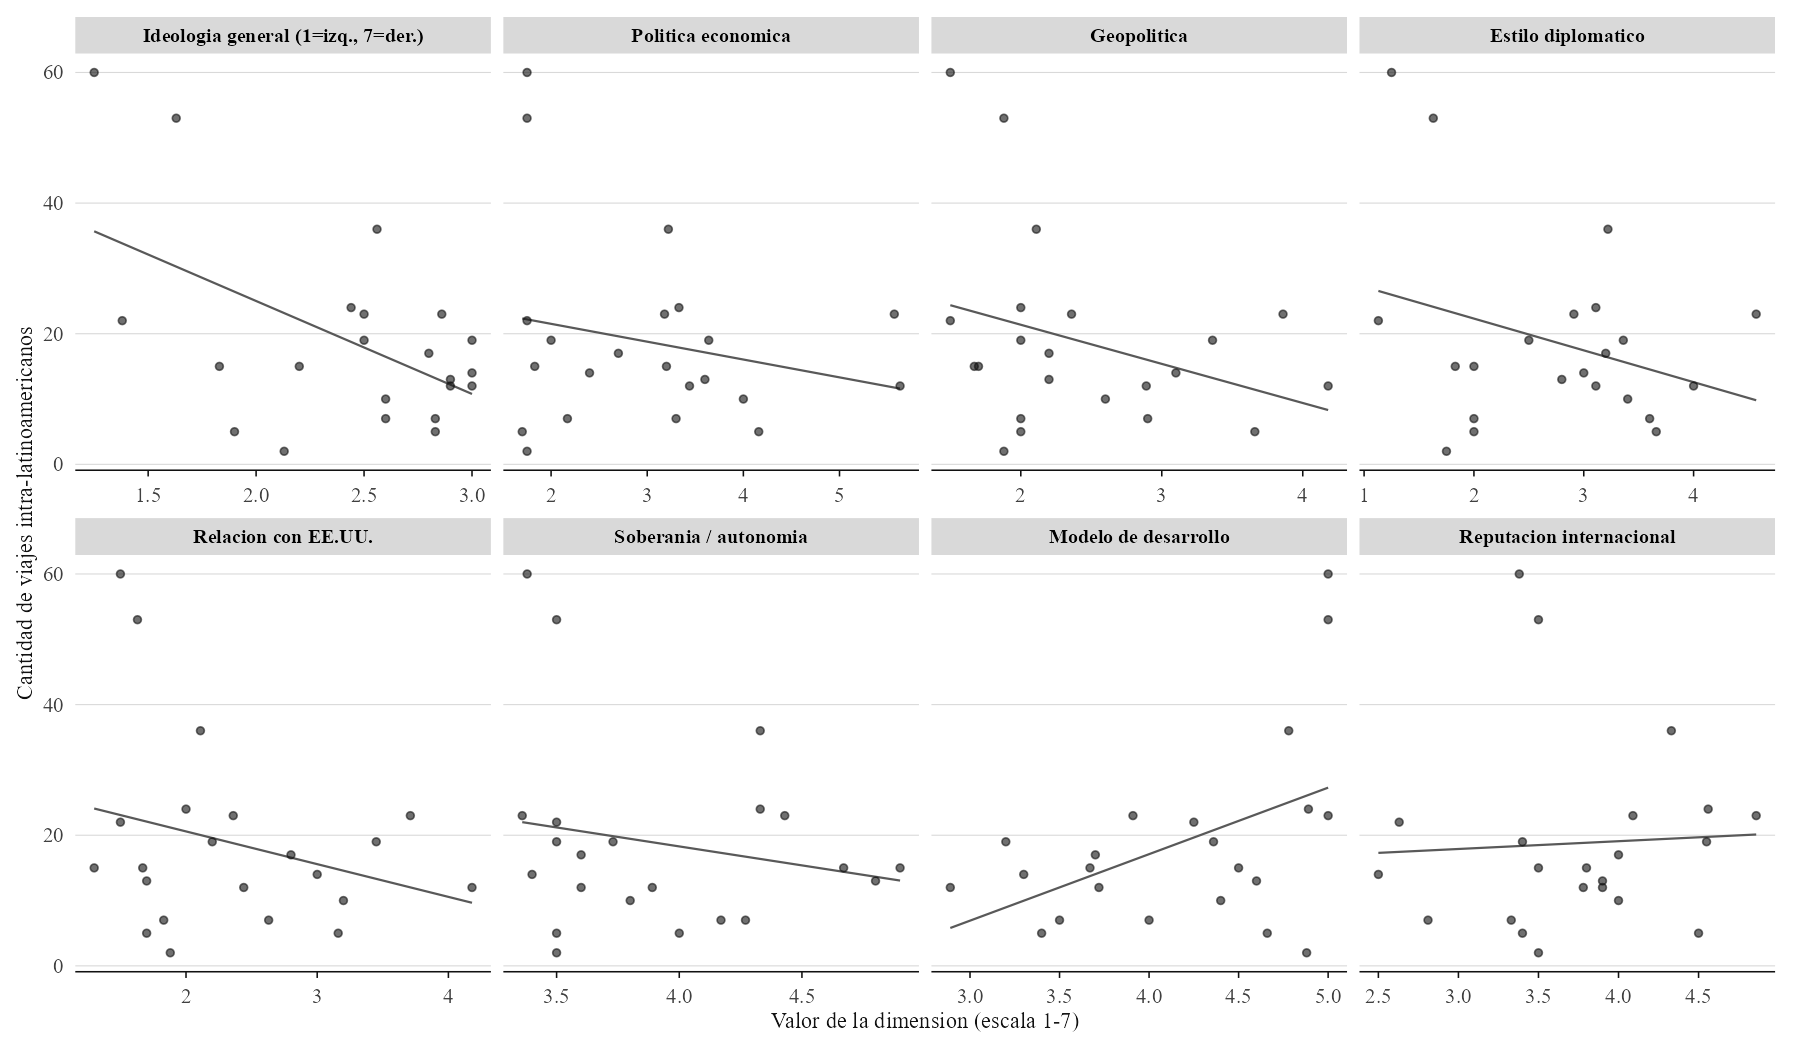
\includegraphics[width=\textwidth]{../08_ANALISIS_R/outputs/18i2_todas_dimensiones_izquierda_absoluto.png}
  \caption{Las ocho dimensiones de ideolog\'ia presidencial vs. cantidad ABSOLUTA de viajes intra-latinoamericanos, restringido a mandato-tramos de ideolog\'ia general BAJA (izquierda, $\leq 3$ en la escala 1-7). Compara con la Figura~\ref{fig:todas-dimensiones-derecha} (\%) y la Figura~\ref{fig:todas-dimensiones-derecha-absoluto}.}
  \label{fig:todas-dimensiones-izquierda-absoluto}
\end{figure}

\begin{figure}[H]
  \centering
  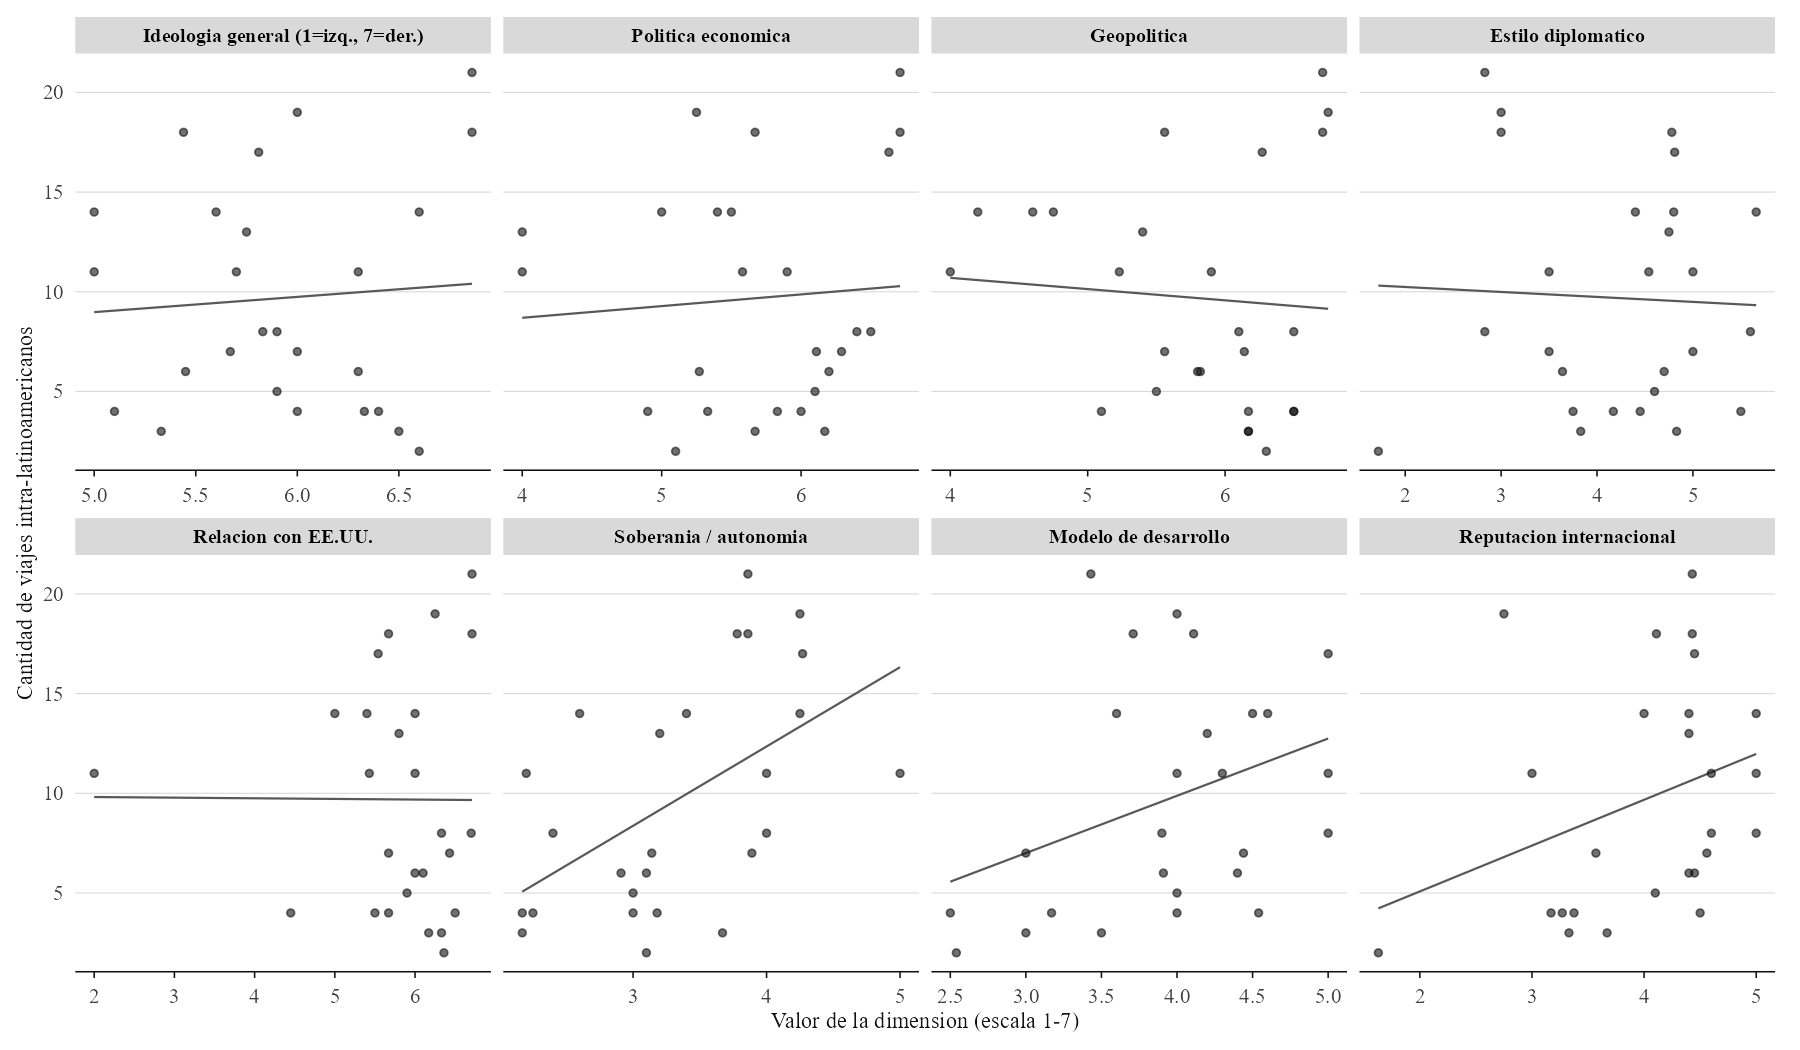
\includegraphics[width=\textwidth]{../08_ANALISIS_R/outputs/18j2_todas_dimensiones_derecha_absoluto.png}
  \caption{Las ocho dimensiones de ideolog\'ia presidencial vs. cantidad ABSOLUTA de viajes intra-latinoamericanos, restringido a mandato-tramos de ideolog\'ia general ALTA (derecha, $\geq 5$ en la escala 1-7).}
  \label{fig:todas-dimensiones-derecha-absoluto}
\end{figure}

\begin{figure}[H]
  \centering
  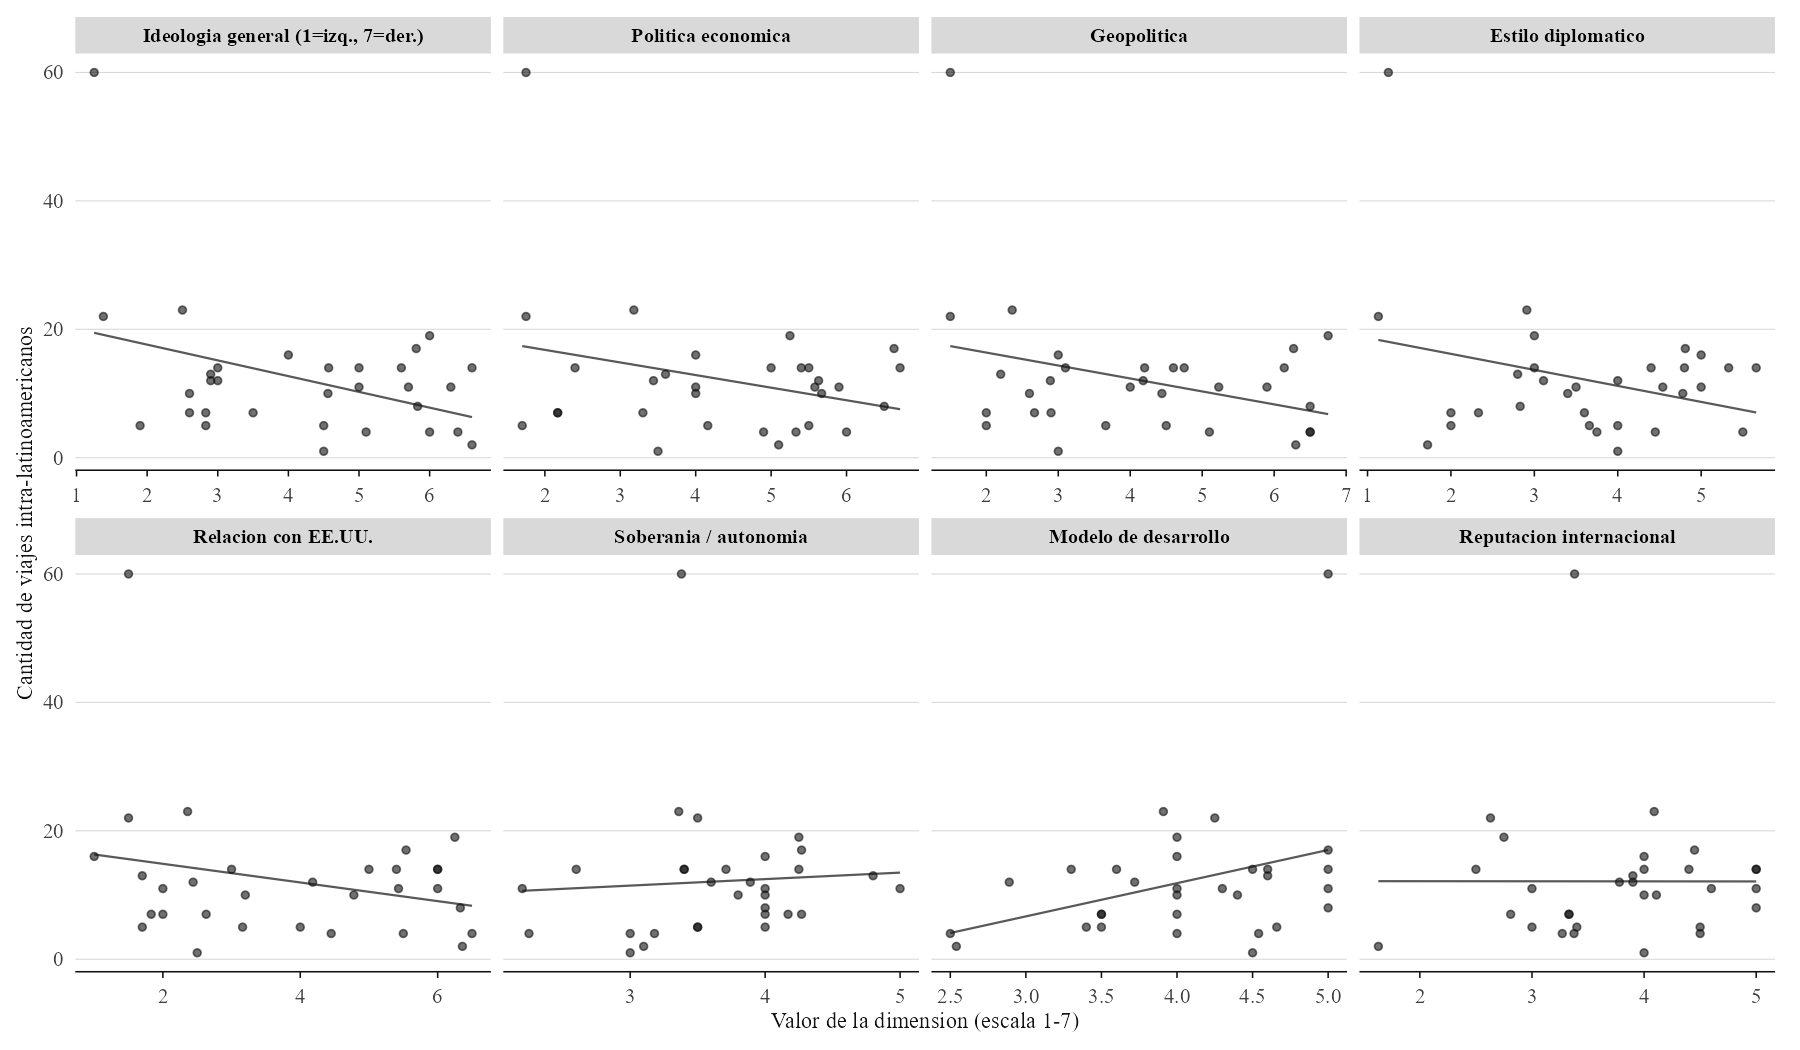
\includegraphics[width=\textwidth]{../08_ANALISIS_R/outputs/18k2_todas_dimensiones_2012_2022_absoluto.png}
  \caption{Las ocho dimensiones de ideolog\'ia presidencial vs. cantidad ABSOLUTA de viajes intra-latinoamericanos, restringido a mandato-tramos que se solapan con la ventana 2012-2022 (los \'ultimos 10 a\~nos con dato de ideolog\'ia disponible).}
  \label{fig:todas-dimensiones-2012-2022-absoluto}
\end{figure}

\begin{figure}[H]
  \centering
  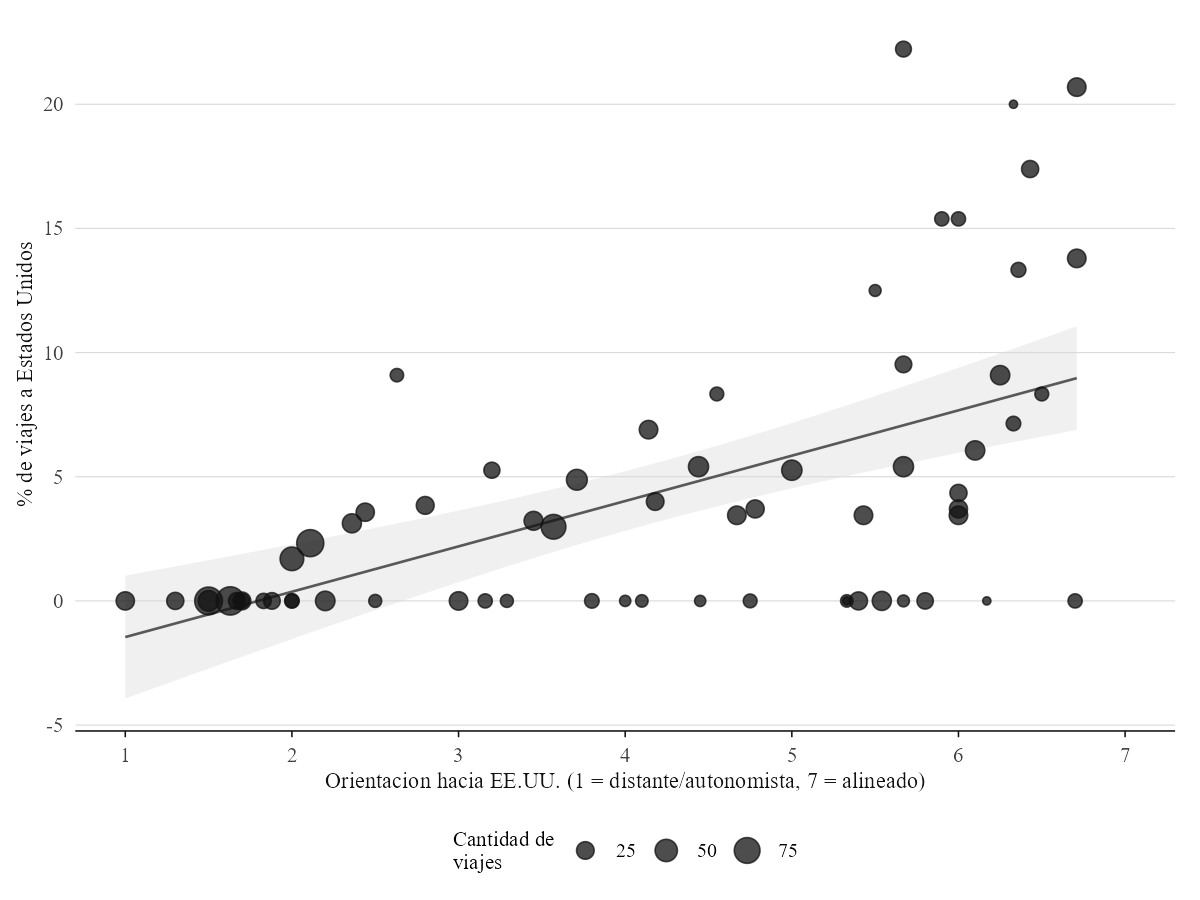
\includegraphics[width=0.85\textwidth]{../08_ANALISIS_R/outputs/18e_usa_vs_pct_viajes_eeuu.png}
  \caption{Validaci\'on cruzada: dimensi\'on ``relaci\'on con EE.\,UU.'' vs. \% de viajes efectivamente dirigidos a Estados Unidos (a diferencia de las Figuras~\ref{fig:ideologia-vs-intralatam} y~\ref{fig:todas-dimensiones-intralatam}, ac\'a la variable dependiente no es el \% intra-latinoamericano sino el \% a Estados Unidos, la que en principio deber\'ia relacionarse m\'as directamente con esta dimensi\'on puntual).}
  \label{fig:usa-vs-pct-eeuu}
\end{figure}

% Figura "bloque ideologico vs intralatam" (boxplot, 18f) ELIMINADA (pedido
% del usuario: "no nos dice mucho").

% latex table generated in R 4.5.1 by xtable 1.8-8 package
% Fri Sep 11 10:51:23 2026
\begin{table}[ht]
\centering
\caption{\colorbox{yellow}{\parbox{\dimexpr\textwidth-2\fboxsep\relax}{Correlaci\'on de Pearson entre la ideolog\'ia general del presidente (1=izq., 7=der.) y el \% de sus viajes dirigidos a Estados Unidos, China y Europa, por mandato-tramo.}}} 
\label{tab:correlacion-destinos}
\begin{tabular}{lrrr}
  \hline
Destino & r\_pearson & valor\_p & n\_mandatos \\ 
  \hline
Estados Unidos & 0.48 & 0.00 &  66 \\ 
  China & 0.14 & 0.27 &  66 \\ 
  Europa & -0.06 & 0.61 &  66 \\ 
   \hline
\end{tabular}
\end{table}% NOTA: caption resaltada en amarillo a pedido del usuario -probablemente se
% elimine este Cuadro en el futuro; revisar antes de la version final.

\begin{figure}[H]
  \centering
  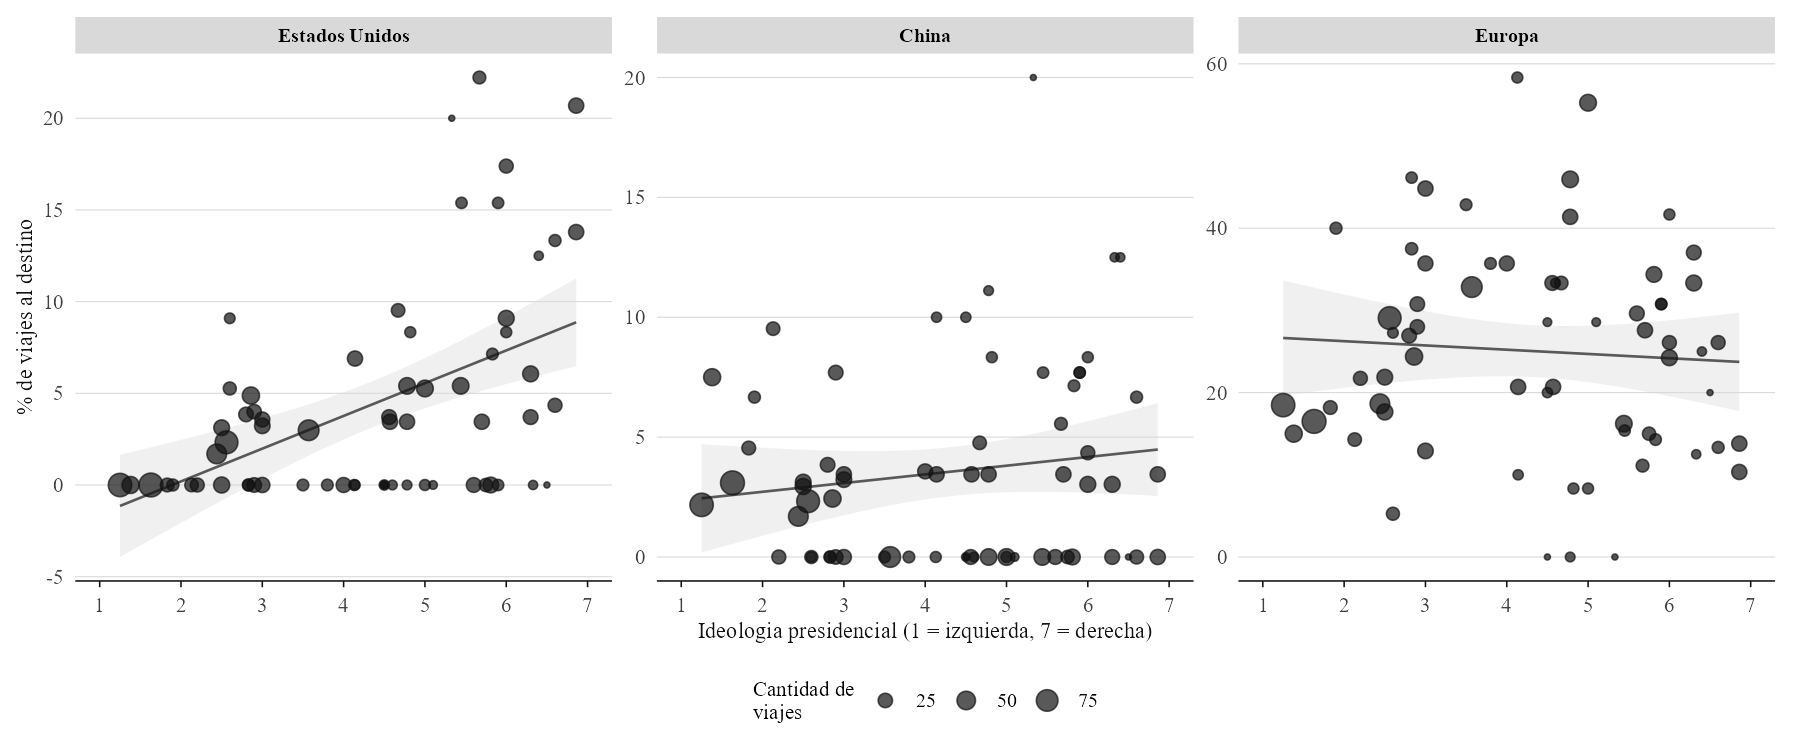
\includegraphics[width=\textwidth]{../08_ANALISIS_R/outputs/18h_ideologia_vs_eeuu_china_europa.png}
  \caption{Ideolog\'ia presidencial general vs. \% de viajes a Estados Unidos, China y Europa, un punto por mandato-tramo. A diferencia de la relaci\'on con el \% intra-latinoamericano (Figura~\ref{fig:ideologia-vs-intralatam}), ac\'a se compara la misma variable X (ideolog\'ia general) contra tres destinos extra-regionales distintos.}
  \label{fig:ideologia-vs-eeuu-china-europa}
\end{figure}

\subsubsection{Homofilia ideol\'ogica en los destinos}

% Pregunta original del usuario: los gobiernos de derecha, tienen mas chances
% de visitar presidentes de la MISMA ideologia que los de izquierda, a lo
% largo del tiempo? Ver 08_ANALISIS_R/graficos_exploratorios.R, seccion 19,
% para el detalle metodologico completo. Se restringe a viajes Sudamerica ->
% Sudamerica con origen Y destino matcheados a la base de ideologia, y
% (2026-09-11, pedido del usuario) EXCLUSIVAMENTE a Visit_Category ==
% "Bilateral" -antes convivian una version "todas las categorias" y una
% version "solo Bilateral" en paralelo, para comparar si el patron de
% homofilia se sostenia al sacar los encuentros multilaterales (la respuesta
% fue si, se sostenia); el usuario decidio dejar solo la version Bilateral
% como version unica y definitiva, porque un viaje a una cumbre multilateral
% no refleja una preferencia bilateral real del presidente por ese destino
% segun su propia ideologia -fue el foro, no una eleccion diadica, lo que lo
% llevo ahi (mismo criterio del Cuadro~\ref{tab:destino-favorito}). El cruce
% diadico -exige ideologia verificada tanto del origen como del destino en la
% misma fecha- en la practica llega hasta 2024, no 2025: el ultimo viaje de
% 19a_homofilia_ideologica_diadico_bilateral.csv es de 2024-12-14.

Esta subsecci\'on cambia la pregunta: en lugar de mirar la orientaci\'on regional agregada de los viajes, compara la ideolog\'ia del presidente que viaja con la del presidente del pa\'is visitado (an\'alisis di\'adico), restringido a viajes \textbf{Bilaterales} entre pa\'ises sudamericanos con ambos lados identificados en la base de ideolog\'ia (se excluyen Multilateral, Other y Sin dato, por el mismo motivo que en la secci\'on anterior: un pa\'is puede acumular visitas por ser sede recurrente de cumbres multilaterales sin que eso refleje una preferencia bilateral real). Se presentan dos versiones del \'indice deliberadamente: una \textbf{sin controlar} (el \% crudo de viajes a la misma ideolog\'ia) y una \textbf{controlando} por la oferta -un \'indice observado/esperado que usa la composici\'on ideol\'ogica real de los destinos disponibles en cada per\'iodo de 5 a\~nos como referencia-. La distinci\'on importa: en per\'iodos donde la mayor\'ia de los gobiernos de la regi\'on comparten un mismo bloque ideol\'ogico (ej. la ``marea rosa'' 2004-2015), ese bloque muestra autom\'aticamente m\'as ``viajes a la misma ideolog\'ia'' solo porque hay m\'as destinos de ese tipo disponibles, no necesariamente porque haya una preferencia real por visitar pares.

% latex table generated in R 4.5.1 by xtable 1.8-8 package
% Fri Sep 11 10:51:23 2026
\begin{table}[ht]
\centering
\caption{\'Indice de homofilia ideol\'ogica, viajes Bilaterales (viajes observados a la misma ideolog\'ia / viajes esperados bajo independencia estad\'istica), por bloque, 1994-2024. Un valor $>1$ indica m\'as visitas ``propias'' de las esperadas por azar.} 
\label{tab:indice-homofilia}
\begin{tabular}{lrrr}
  \hline
Bloque & Viajes\_observados & Viajes\_esperados & Indice\_homofilia \\ 
  \hline
Izquierda & 142 & 93.90 & 1.51 \\ 
  Centro &  45 & 39.80 & 1.13 \\ 
  Derecha &  91 & 63.00 & 1.44 \\ 
   \hline
\end{tabular}
\end{table}
\begin{figure}[H]
  \centering
  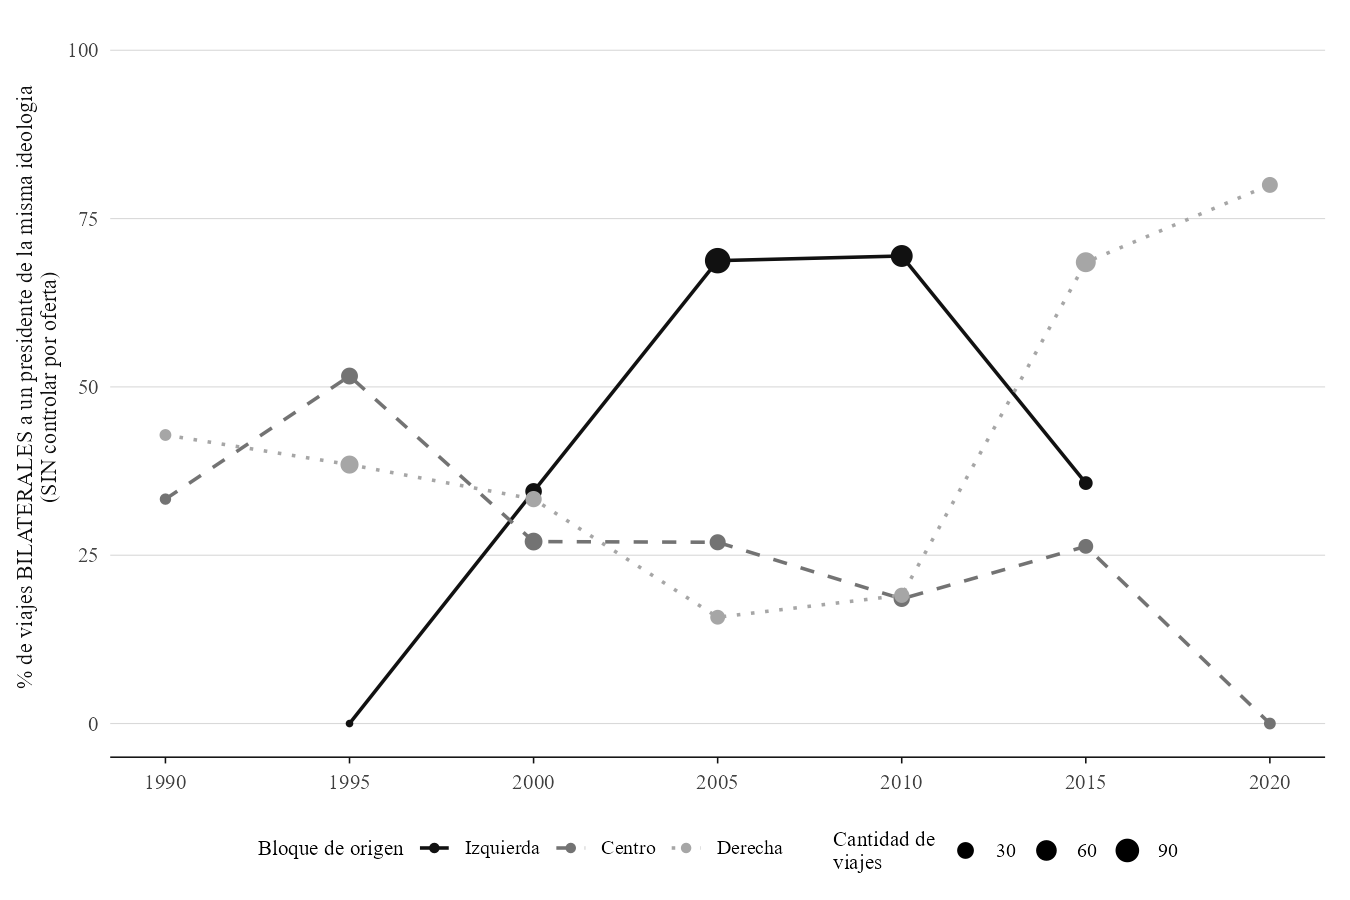
\includegraphics[width=0.85\textwidth]{../08_ANALISIS_R/outputs/19c_homofilia_sin_controlar_bilateral.png}
  \caption{\% de viajes Bilaterales a un presidente de la misma ideolog\'ia, por bloque de origen y per\'iodo, SIN controlar por la oferta ideol\'ogica disponible en cada momento.}
  \label{fig:homofilia-sin-controlar}
\end{figure}

\begin{figure}[H]
  \centering
  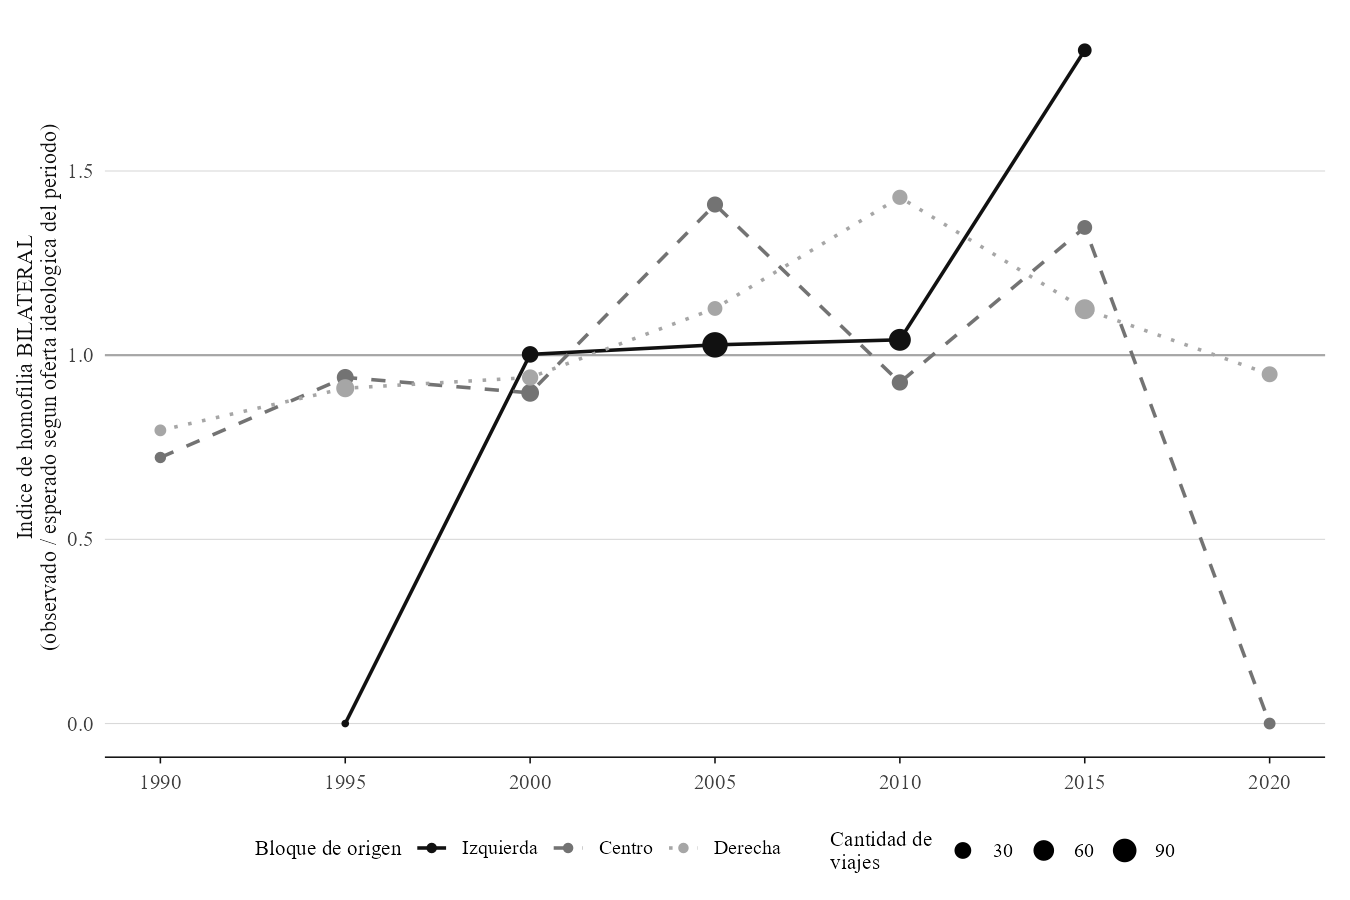
\includegraphics[width=0.85\textwidth]{../08_ANALISIS_R/outputs/19e_homofilia_controlando_bilateral.png}
  \caption{\'Indice de homofilia (observado/esperado) por bloque de origen y per\'iodo, CONTROLANDO por la composici\'on ideol\'ogica real de los destinos disponibles en cada per\'iodo de 5 a\~nos. La l\'inea horizontal en 1 marca el nivel esperado por azar.}
  \label{fig:homofilia-controlando}
\end{figure}

\begin{figure}[H]
  \centering
  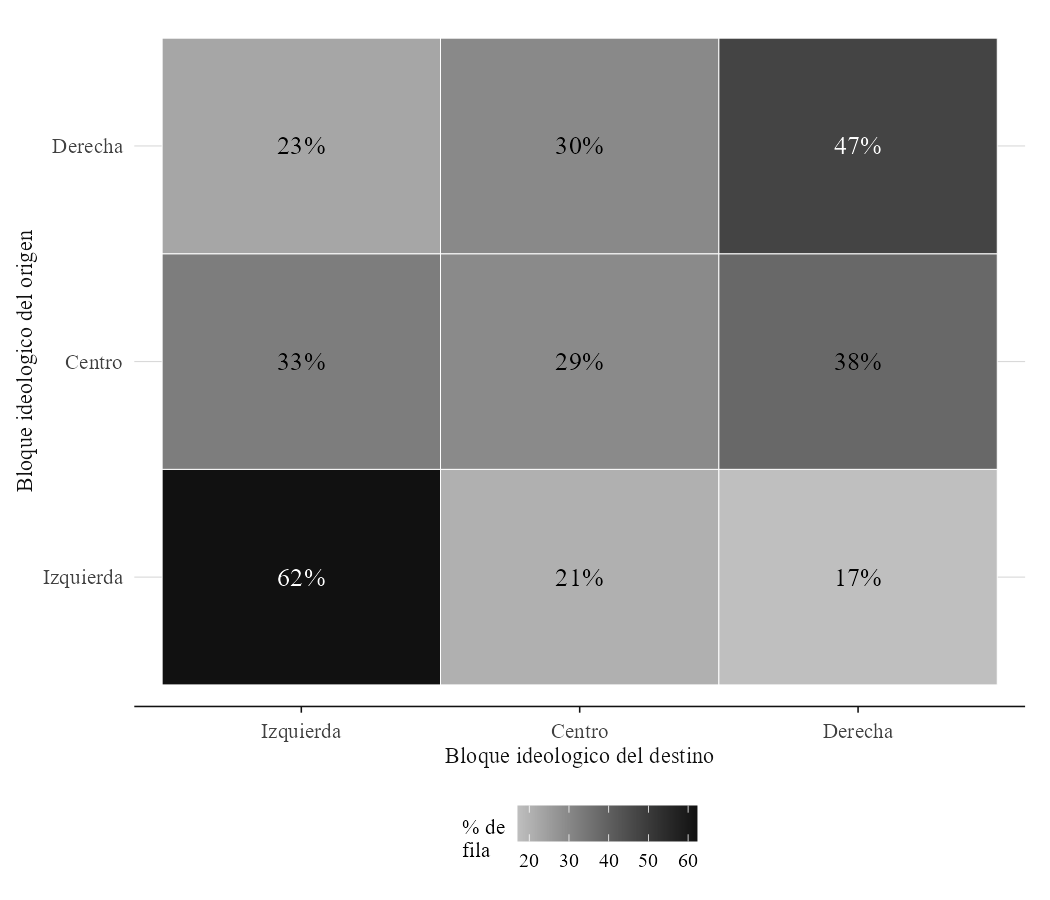
\includegraphics[width=0.6\textwidth]{../08_ANALISIS_R/outputs/19f_matriz_origen_destino_bilateral.png}
  \caption{Matriz de bloque ideol\'ogico del origen (fila) vs. bloque ideol\'ogico del destino (columna), \% de fila, viajes Bilaterales, todo el per\'iodo 1994-2024 en conjunto.}
  \label{fig:matriz-origen-destino}
\end{figure}

\subsubsection{Ideolog\'ia en d\'iadas con Europa (dataset de Herre)}

% NUEVO (2026-09-11, pivot "Diplomacia Presidencial", punto 7). Pregunta: la
% homofilia ideologica de la subseccion anterior -solo Sudamerica-Sudamerica-
% se sostiene tambien cuando el destino es un lider europeo? Ver
% 08_ANALISIS_R/graficos_exploratorios.R, seccion 22, para el detalle
% metodologico completo. Limitaciones confirmadas y aceptadas por el usuario
% (no son bugs, son decisiones de alcance):
%  (a) El dataset de Herre et al. (2023, "Identifying Ideologues") cubre
%      1945-2020; todo viaje Bilateral a Europa posterior a 2020 queda
%      necesariamente sin clasificar del lado europeo (se cuantifica en
%      22_diadas_sudamerica_europa.csv / n_posterior_2020 en la consola de R).
%  (b) Universo: TODOS los paises europeos visitados (no solo la UE ni un
%      subconjunto), por decision explicita del usuario.
%  (c) Se usa la variable leader_ideology de Herre (el "lider efectivo"
%      segun Archigos, ej. el Presidente en sistemas semipresidenciales como
%      Francia) y NO hog_ideology (el jefe de gobierno formal), porque
%      leader_ideology aproxima mejor a la contraparte que un presidente
%      sudamericano efectivamente trata en una visita bilateral, y porque
%      mantiene la simetria conceptual con nuestra propia base (un
%      presidente sudamericano frente a un "lider efectivo" europeo).
%  (d) Sin cobertura en Herre para Santa Sede/Vaticano y M\'onaco
%      (microestados) ni para Checoslovaquia (disuelta en 1993, fuera del
%      rango practico de nuestra ventana 1994+); estos casos quedan sin
%      clasificar del lado europeo, igual que (a).
%  (e) Cruce por a\~no calendario (a\~no del viaje vs. a\~no-pa\'is de Herre),
%      no por fecha exacta -aproximacion aceptada dado que Herre es un panel
%      pa\'is-a\~no, no un panel con fechas de cambio de gobierno-.
% Unico ajuste de nombres necesario (crosswalk): "Czechia" (nuestra base) =
% "Czech Republic" (Herre). El resto de los nombres de pa\'ises europeos
% coincide exactamente entre ambas bases (verificado).

Como extensi\'on de la pregunta anterior, cabe preguntarse si el patr\'on de homofilia ideol\'ogica sudamericana se sostiene tambi\'en hacia afuera de la regi\'on: \textquestiondown los presidentes sudamericanos de un bloque ideol\'ogico visitan, en sus viajes Bilaterales a Europa, con mayor frecuencia a l\'ideres europeos del mismo bloque? Para responder esto se cruz\'o cada viaje Bilateral de un presidente sudamericano a Europa con la ideolog\'ia del l\'ider europeo efectivamente en el poder ese a\~no, usando el dataset ``Identifying Ideologues'' (Herre et al., 2023)\footnote{Pendiente: agregar esta referencia a Zotero para que quede incorporada a \texttt{referencias.bib} y pueda citarse formalmente en la versi\'on final.}, que codifica la ideolog\'ia (izquierda/centro/derecha) de los l\'ideres nacionales a nivel mundial en un panel pa\'is-a\~no 1945-2020. Dado que este dataset no cubre 2021 en adelante, los viajes posteriores a esa fecha quedan fuera del an\'alisis di\'adico (se conservan en el resto del paper, que no depende de esta fuente).

% latex table generated in R 4.5.1 by xtable 1.8-8 package
% Fri Sep 11 10:51:23 2026
\begin{table}[ht]
\centering
\caption{Test de independencia chi-cuadrado entre el bloque ideol\'ogico del presidente sudamericano y el bloque ideol\'ogico del l\'ider europeo visitado, viajes Bilaterales Sudam\'erica-Europa con ambos lados clasificados (Herre 2023, cobertura hasta 2020).} 
\label{tab:chi2-europa}
\begin{tabular}{rrrr}
  \hline
chi2 & df & valor\_p & n\_diadas \\ 
  \hline
5.90 &   4 & 0.21 & 343 \\ 
   \hline
\end{tabular}
\end{table}
\begin{figure}[H]
  \centering
  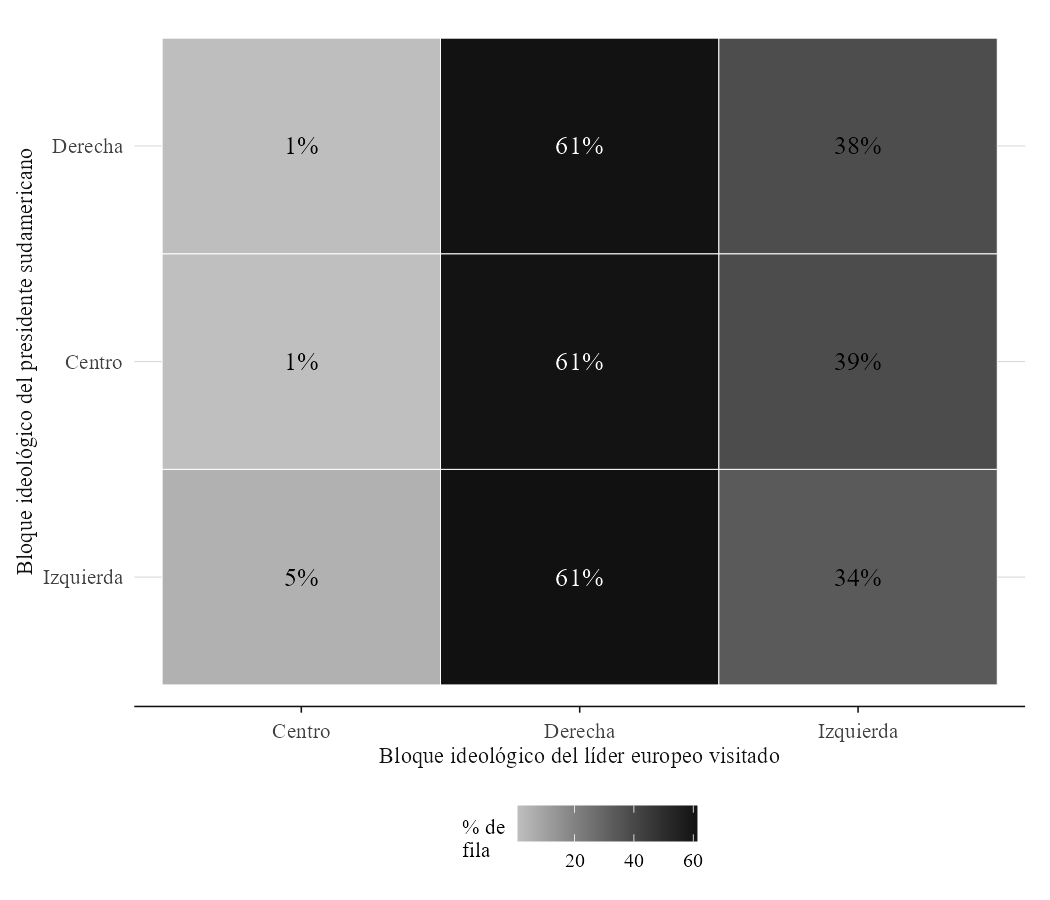
\includegraphics[width=0.6\textwidth]{../08_ANALISIS_R/outputs/22b_matriz_sudamerica_europa.png}
  \caption{Matriz de bloque ideol\'ogico del presidente sudamericano (fila) vs. bloque ideol\'ogico del l\'ider europeo visitado (columna), \% de fila, viajes Bilaterales a Europa con ambos lados clasificados seg\'un Herre (2023), cobertura hasta 2020.}
  \label{fig:matriz-sudamerica-europa}
\end{figure}

\subsubsection{Comercio}

% PENDIENTE (2026-09-11, pivot "Diplomacia Presidencial", punto 3): el
% usuario indico explicitamente que todavia tiene que sumar una base de
% datos de comercio bilateral ("tengo que sumar una base de datos aca").
% Candidatos tipicos para esta pieza (a confirmar con el usuario cuando
% aporte la base): UN Comtrade (bilateral, por par de paises y anio),
% CEPII BACI, o series de comercio exterior de ALADI/CEPAL para Sudamerica.
% Una vez integrada, el analisis deberia seguir el mismo patron que
% Ideologia (Secci\'on~\ref{sec:ideologia-viajes}, si se define un label) y
% Cercania: correlacionar el volumen de comercio bilateral del par
% origen-destino con la frecuencia/probabilidad de viaje bilateral a ese
% mismo destino, por mandato-tramo.

Esta subsecci\'on queda pendiente: falta incorporar una base de comercio bilateral (candidatos: UN Comtrade, CEPII BACI, o series de ALADI/CEPAL) para poder correlacionar el volumen de comercio entre cada par de pa\'ises con la frecuencia de viajes bilaterales entre ellos, siguiendo el mismo enfoque de las dos subsecciones anteriores.

\section{Discusi\'on}
% TODO. Conectar los hallazgos con el marco teorico: interpretar quiebres
% con \citep{merkeForeignPolicyChange2020} (ideologia presidencial explica
% cambios de PE), la caida de multilateralismo regional con
% \citep{nolteSummitsPlainsCrisis2021, barrosCrisisSouthAmerican2021}, casos especificos con
% \citep{merkeRightWingPopulismStrategic2026, barrenengoaPoliticaExteriorGobierno2023, romualdosilvaAviaoComPouco2020,
% gomessaraivaBrazilianForeignPolicy2010}, y el contexto reciente con
% \citep{gonzalezDesconciertoLatinoamericanoFrente2026}.

\section{Conclusi\'on}
% TODO.

\printbibliography

\end{document}
